\section{Performance}
\label{sec:perf}

The performance of the ART and MM TP in this note is described relative to the full MMFE8 and scintillator readout, which is to say, the efficiency and resolution is not measured absolutely. For each cosmic muon event, the scintillator is required to have good data quality, and the full MMFE8 readout is required to record a track with at least two clusters in the $X$-planes on opposite quadruplets and at least two clusters in the stereo planes. Every event passing this criteria should create a trigger in the MM TP.

\subsection{Basic performance}
\label{sec:perf-basic}

The MM TP shows excellent efficiency for finding a trigger given the criteria described above. Figure~\ref{fig:lowlevel} shows the efficiency for finding a trigger as a function of time (left) and the number of hits in the trigger as a function of time (right). Both figures indicate stable performance throughout the run.

The triggers created by the MM TP are also in good agreement with the expectation from the full MMFE8 readout, as shown in Figure~\ref{fig:lowlevel}. The angular distribution (right) is nearly identical between the MM TP and the MMFE8s, where the angle of the MM TP is the angle evaluated in the FPGA, and the angle of the MMFE8 track is the angle calculated offline. The hit multiplicity (left) is similar between the MM TP and the MMFE8s, though on average the MM TP records fewer hits per track. This is due to the 7 BC collection window discussed in Section~\ref{sec:alg-finder}. Occasionally, this window is still not large enough, and an ART hit arrives too late to be considered for the trigger. The collection window is also likely the cause of the sub-percent inefficiency observed in Figure~\ref{fig:lowlevel}.

\begin{figure}[!htpb]
  \begin{center}
    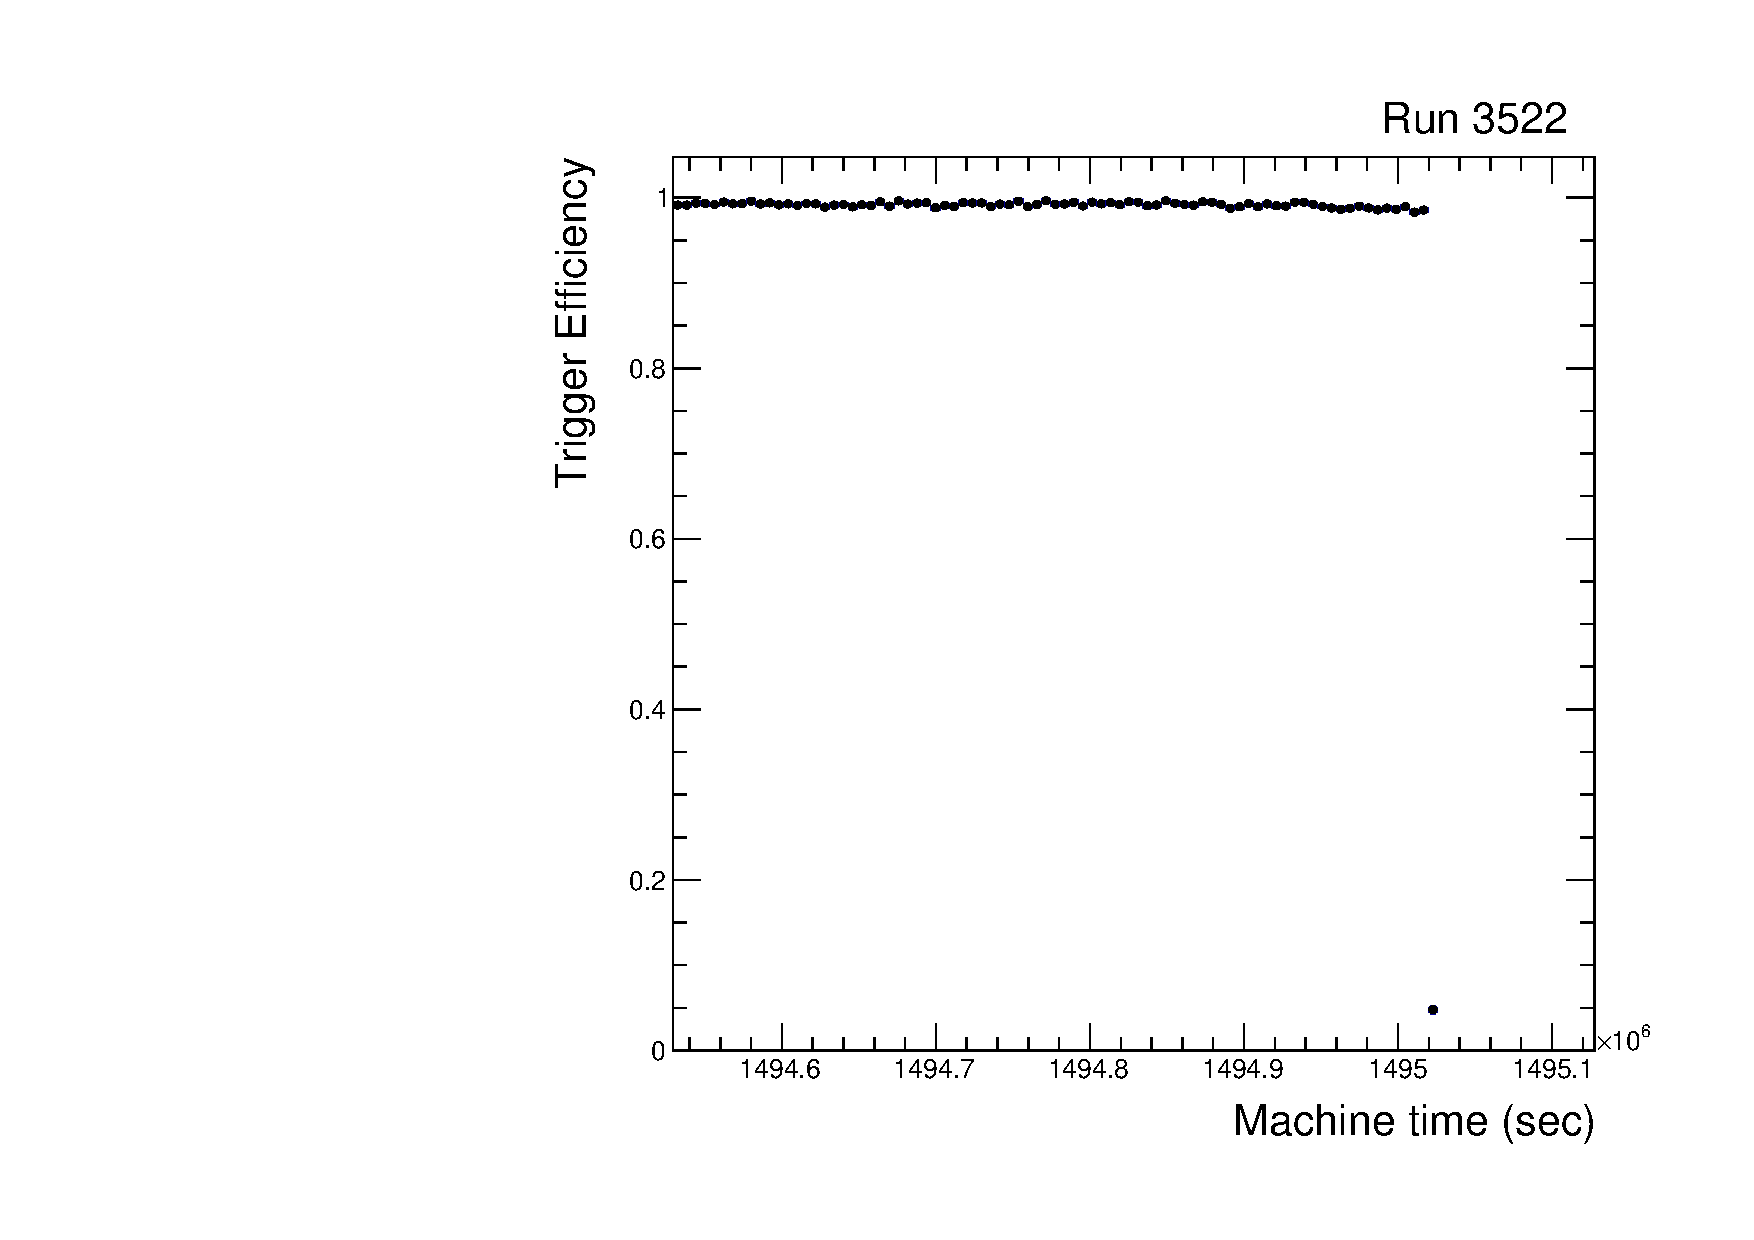
\includegraphics[width=0.4\textwidth]{figures/gbtanalysis3522/tpeff.pdf}
    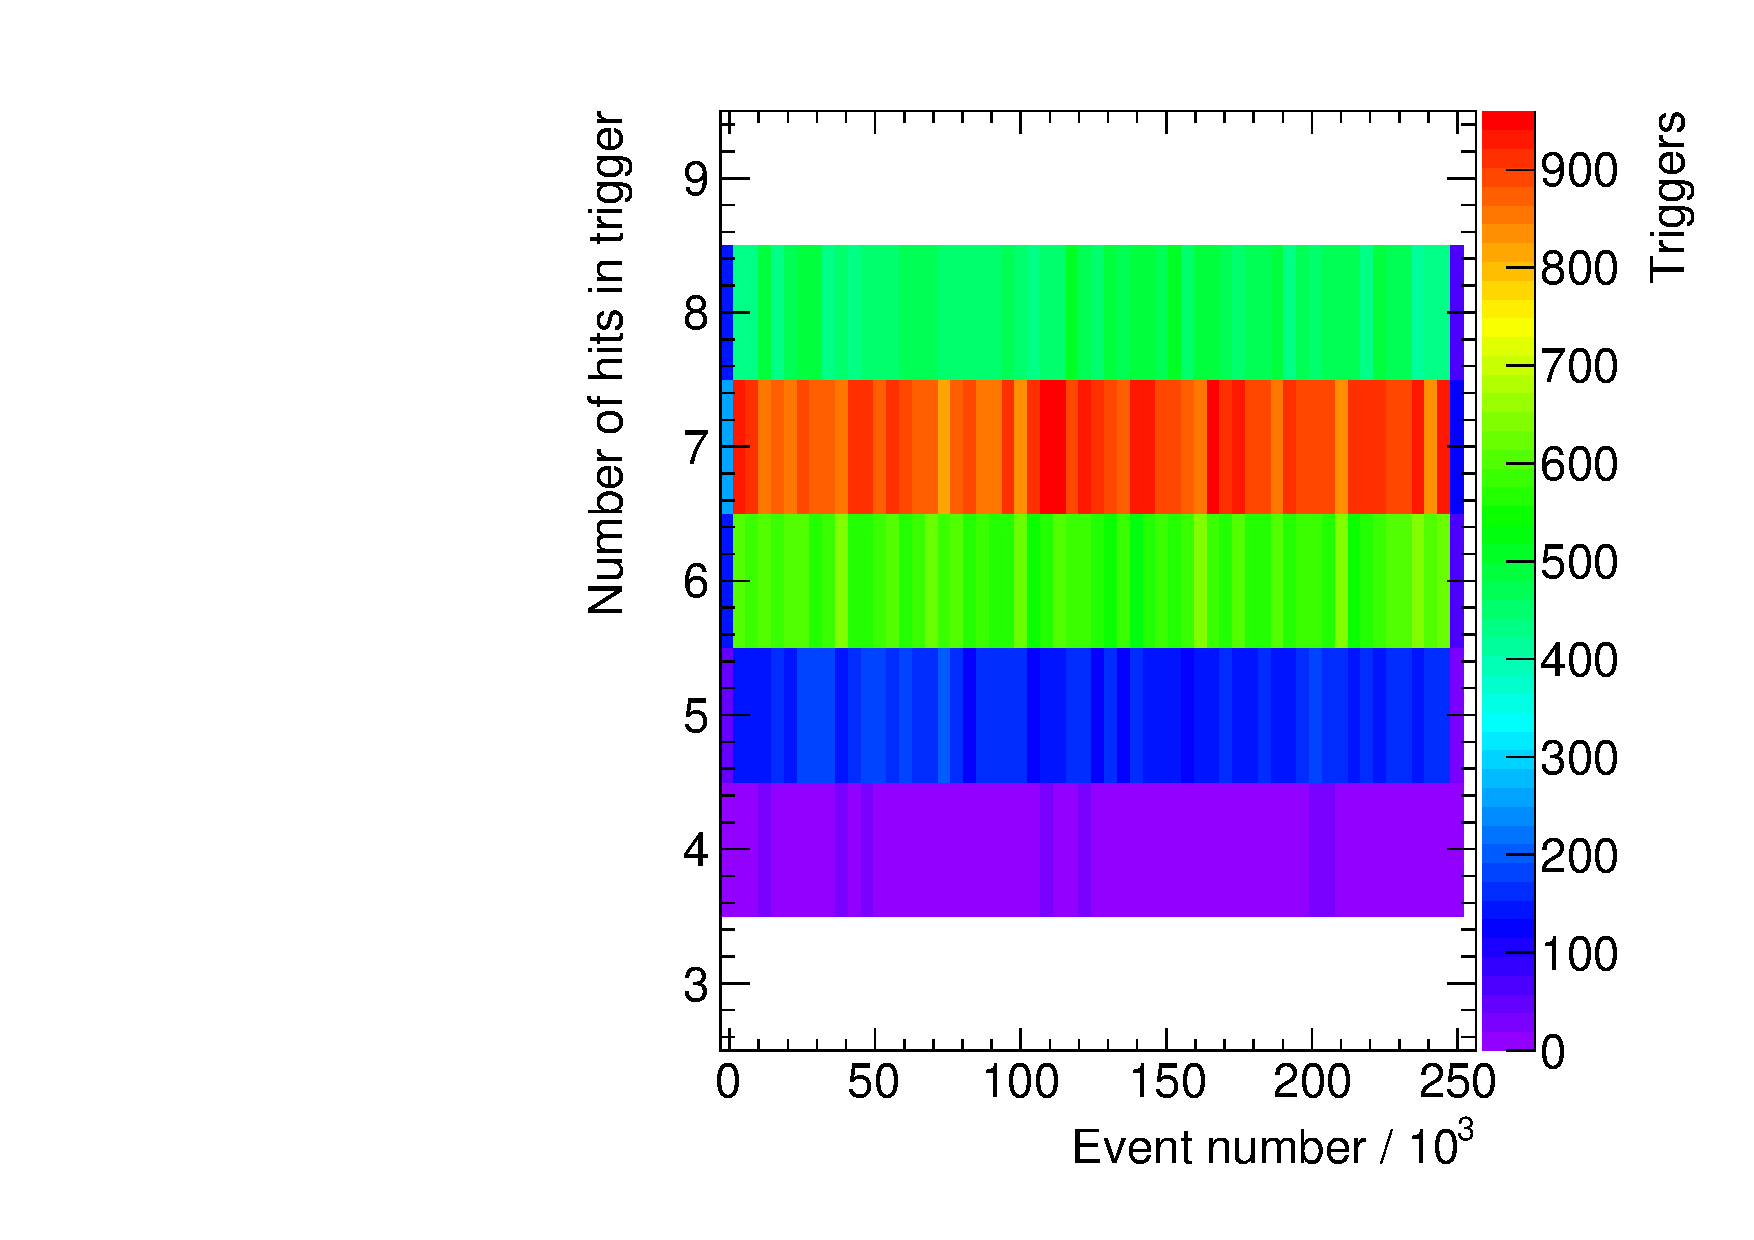
\includegraphics[width=0.4\textwidth]{figures/tuna_analysis/trigger_hits_vs_event.pdf}
  \end{center}
  \vspace{-10pt}
  \caption{The efficiency of a trigger to be matched to a full readout event versus time (left) and the number of hits in the trigger as a function of time (right). Both figures show stable data-taking.}
  \label{fig:lowlevel}
\end{figure}

\begin{figure}[!htpb]
  \begin{center}
    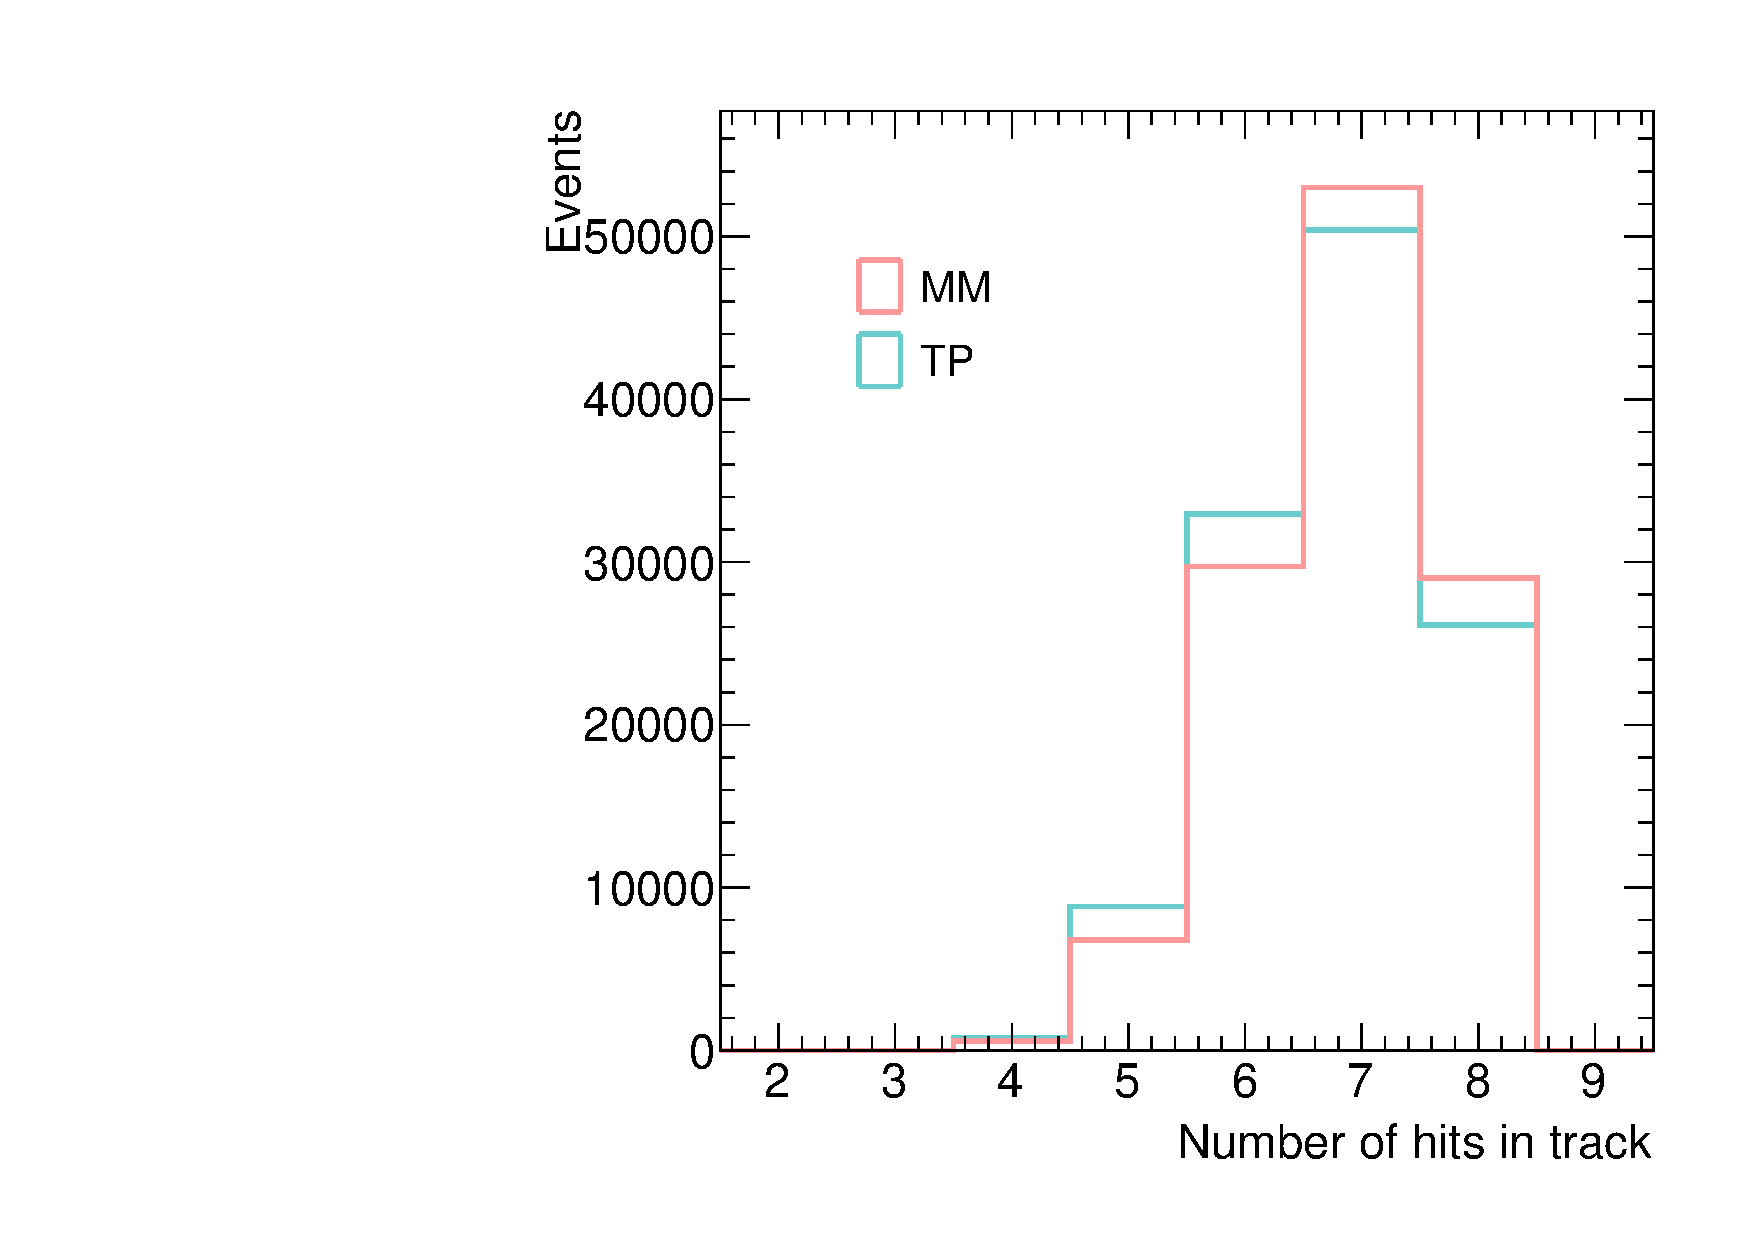
\includegraphics[width=0.4\textwidth]{figures/tuna_analysis/trigger_nart.pdf}
    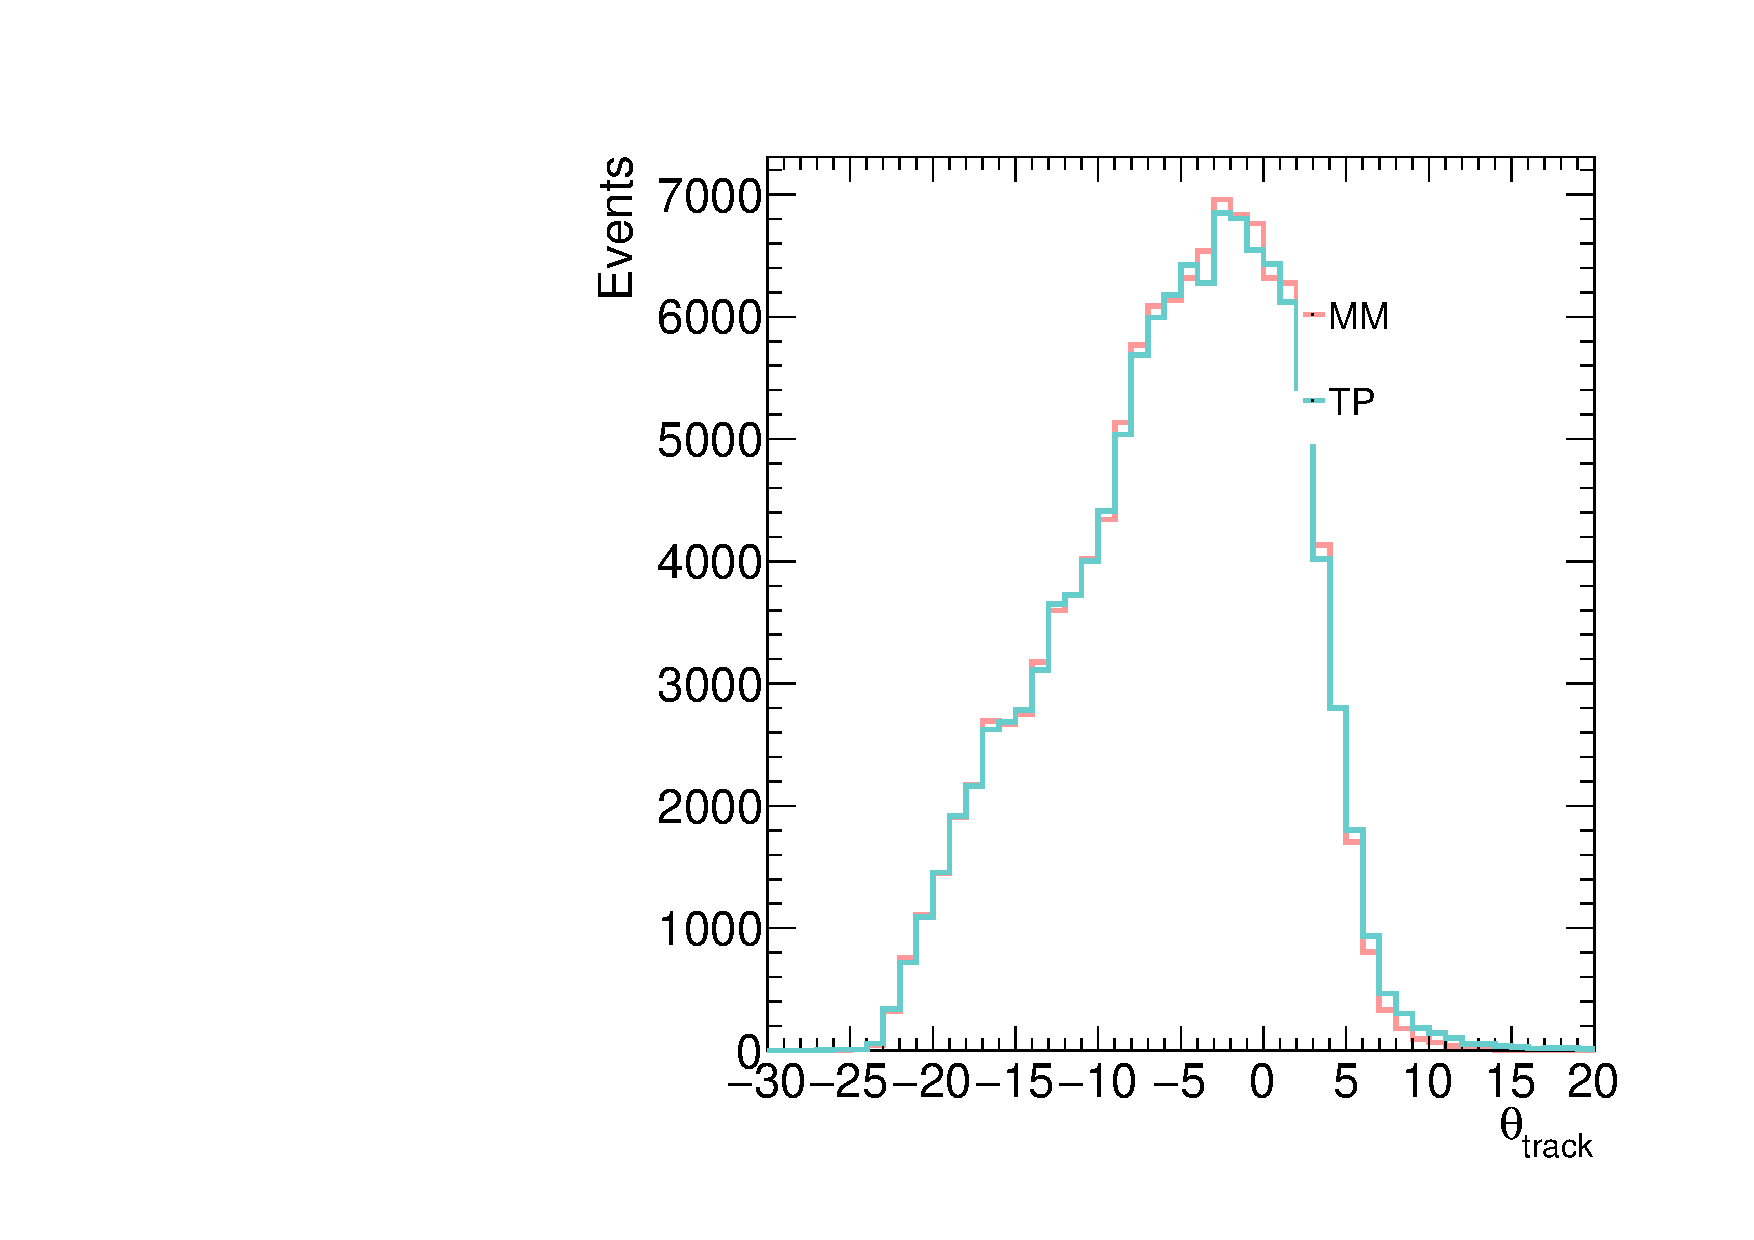
\includegraphics[width=0.4\textwidth]{figures/gbtanalysis3522/ang.pdf}
  \end{center}
  \vspace{-10pt}
  \caption{The number of hits in the MM TP and MM FE tracks (left) and the angle of the tracks (right). The track found by the trigger closely resembles the track found by the full readout, though with slightly fewer hits on average.}
  \label{fig:tp_vs_fe}
\end{figure}

\subsection{Offline roads}
\label{sec:perf-roads}

An additional trigger quality requirement is considered when measuring the resolution of the MM TP. As discussion in Section~\ref{sec:alg-finder}, the road size configured in the FPGA is 1 VMM, or effectively 3 VMMs when including neighboring roads. This allows muons with large incident angle to form triggers in the MM TP, but it is also vulnerable to background hits since the effective road is much larger than needed for a downward-going muon. This vulnerability is less relevant for the NSW implementation of the algorithm because it will use \textit{slope-roads}, which is equivalent to only triggering on downward-going muons when using simple, strip-based roads.

To avoid this vulnerability, the resolution measured is presented in two ways. First, the resolution measured by the MM TP is shown unadulterated. Second, the resolution is shown for triggers which satisfy \textit{offline roads}, to emulate the slope-roads of the NSW implementation. Offline roads are defined relative to the reference track of the full MMFE8 readout. The position of this track is evaluated at each layer, and a road is created around this position. The offline roads in this note are defined as 16 strips (1/4 VMM), with neighbors on either side, which is approximately the size of the slope-roads suggested for the NSW. Therefore an ART hit on a given layer must be within 24 strips of the track to ``satisfy'' the road. A trigger is said to satisfy the offline road if all the hits of the trigger satisfy the road individually.

An important caveat is that even slope-roads cannot be simply defined for stereo planes. Unlike horizontal strips, the slope of a stereo strip measured at one edge of the wedge is different than the slope measured at the other edge. The MM TP defines the slope of a stereo strip as the slope evaluated in the center of the wedge, and as the road size is made smaller, it can become inefficient for tracks traversing the wedge near the edges. Therefore the road size for stereo planes must be larger than for horizontal planes.

In this note, the offline stereo road is made larger by approximately the amount which will be needed at the NSW.

\begin{figure}[!htpb]
  \begin{center}
    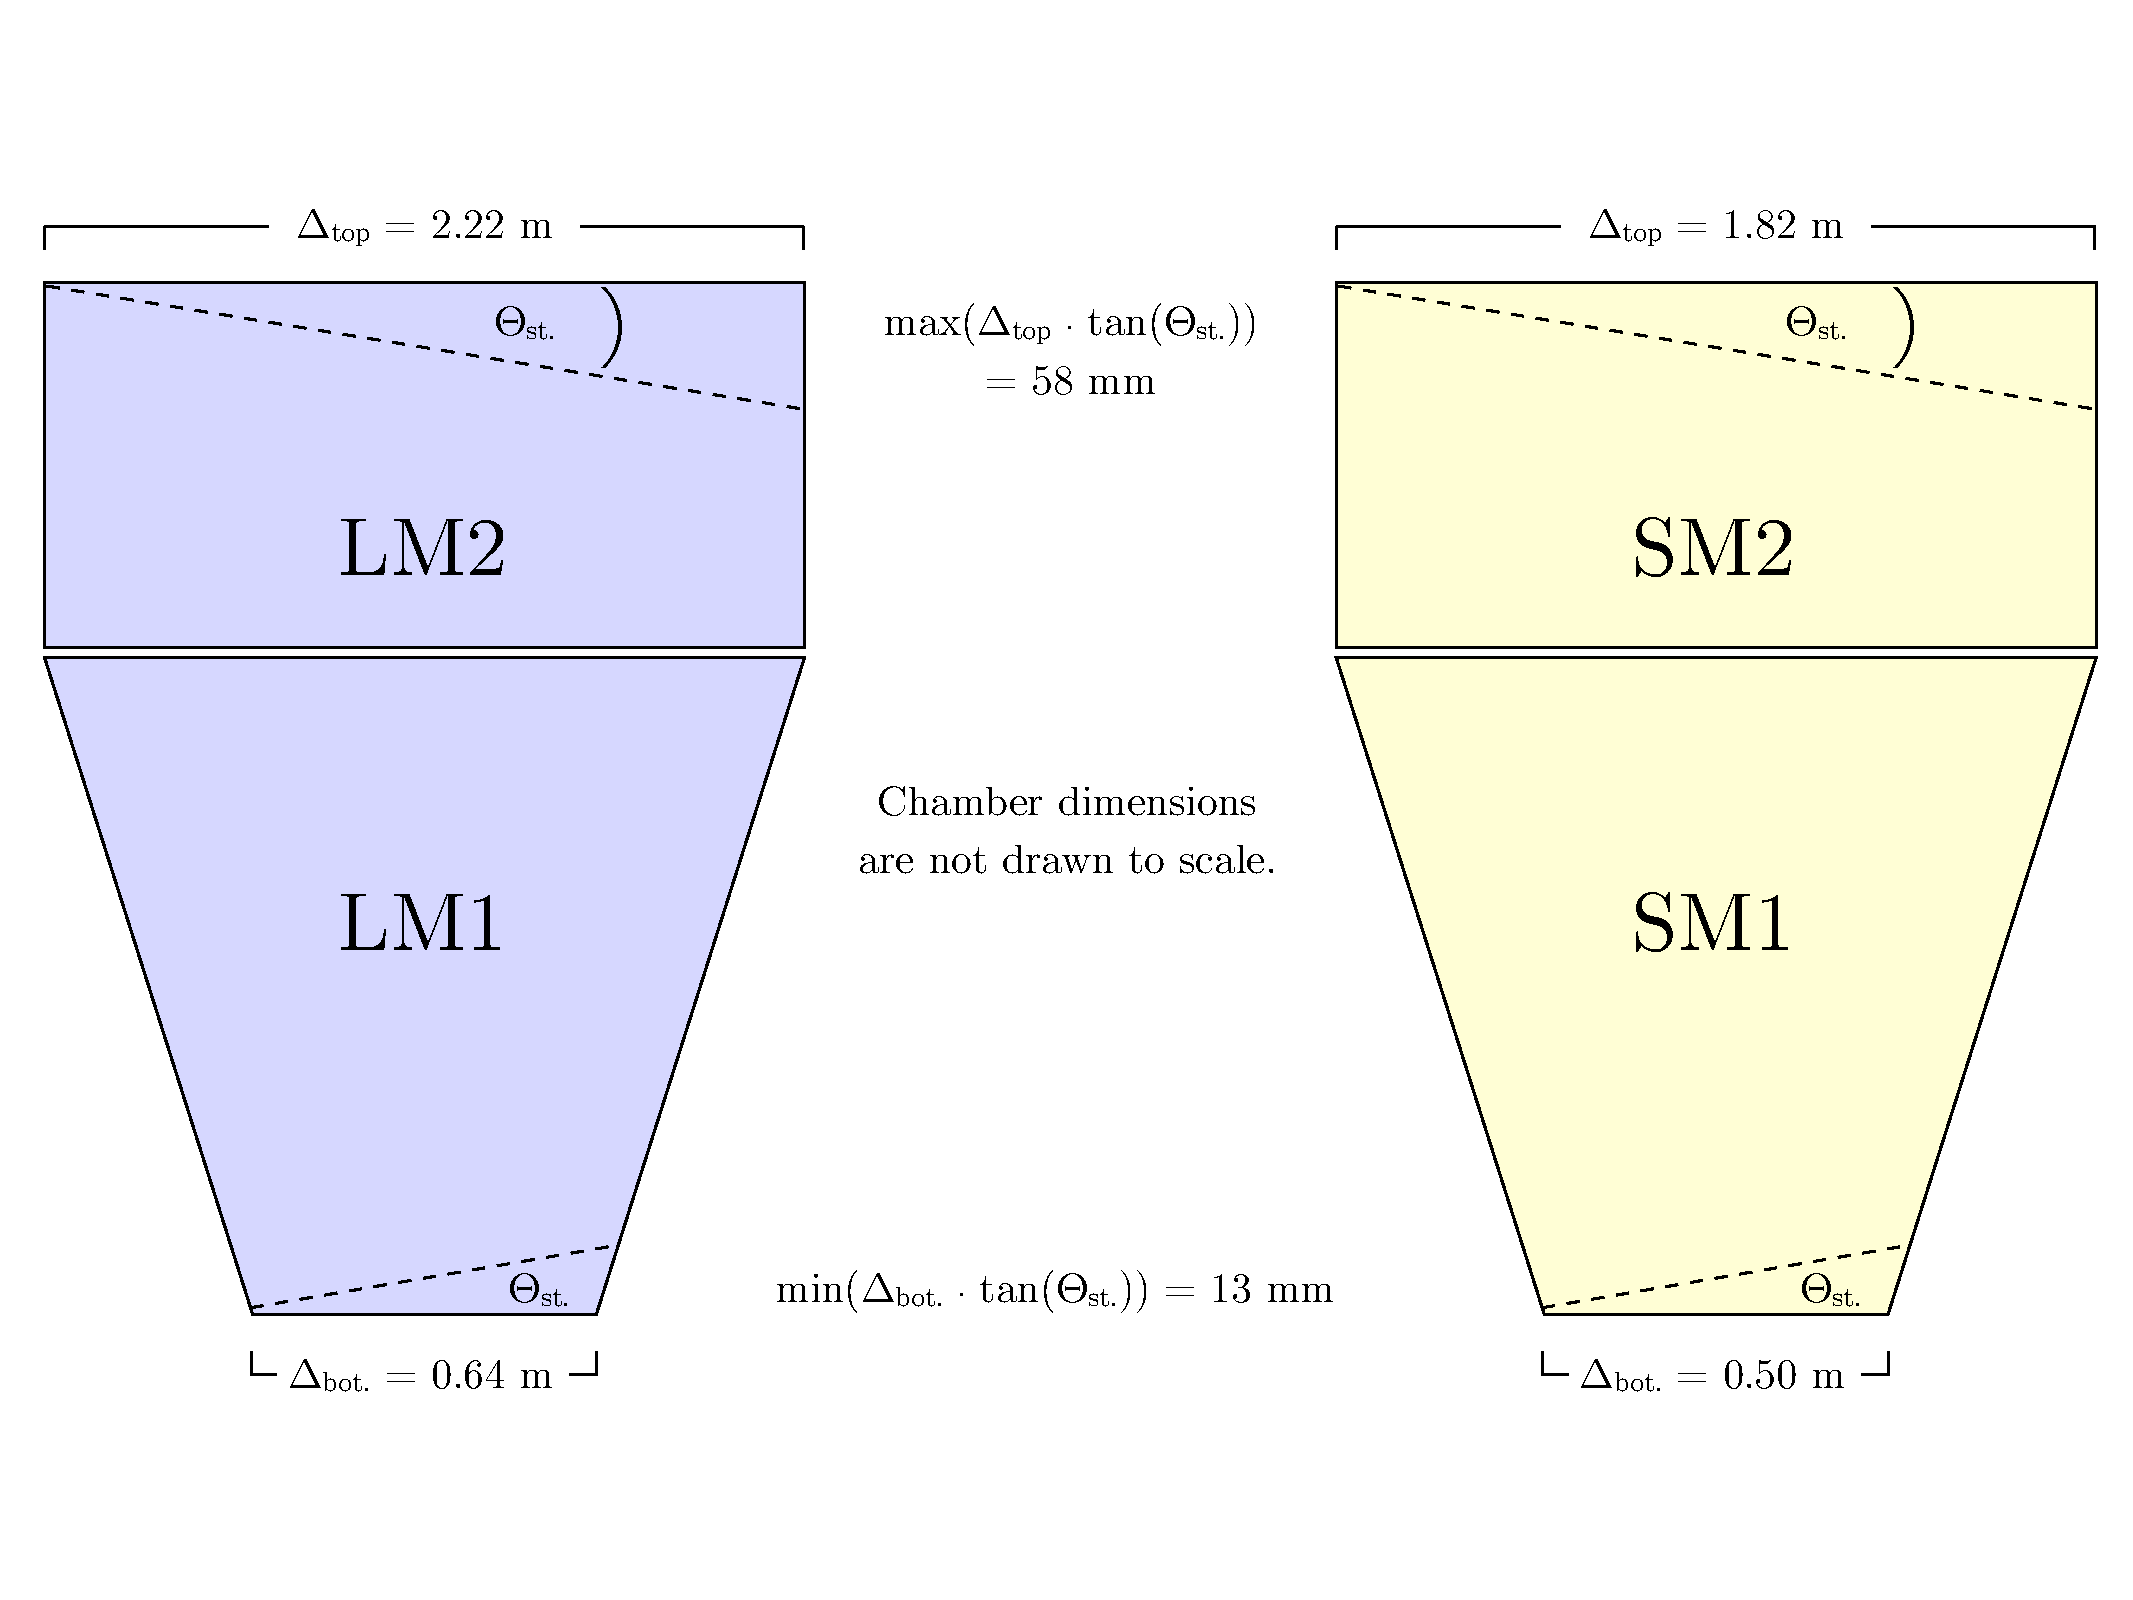
\includegraphics[width=1.0\textwidth]{figures/cartoons/stereo_roads.pdf}
  \end{center}
  \vspace{-10pt}
  \caption{}
  \label{fig:stereo_roads}
\end{figure}

\subsection{Spatial and angular resolution}
\label{sec:perf-res}

\begin{figure}[!htpb]
  \begin{center}
    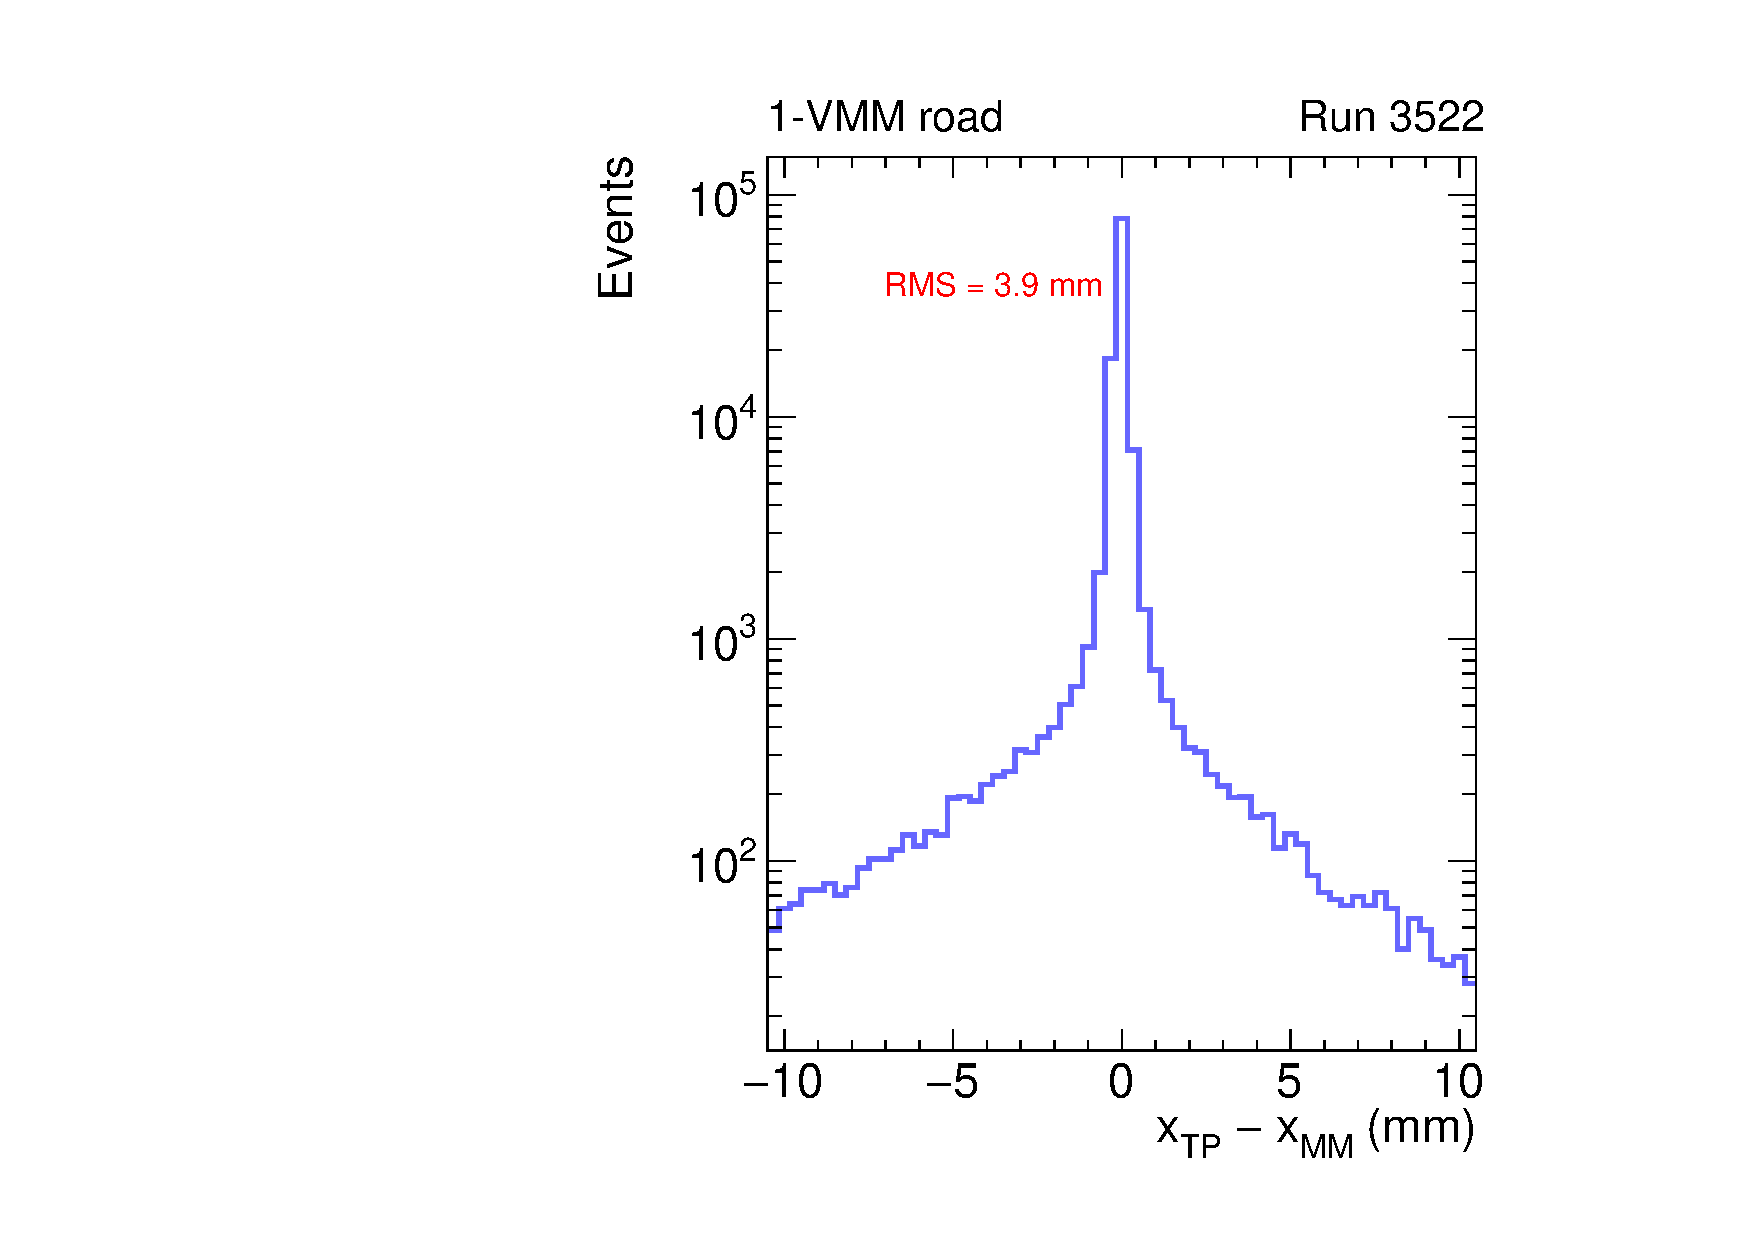
\includegraphics[width=0.4\textwidth]{figures/gbtanalysis3522/TP_xres_full.pdf}
    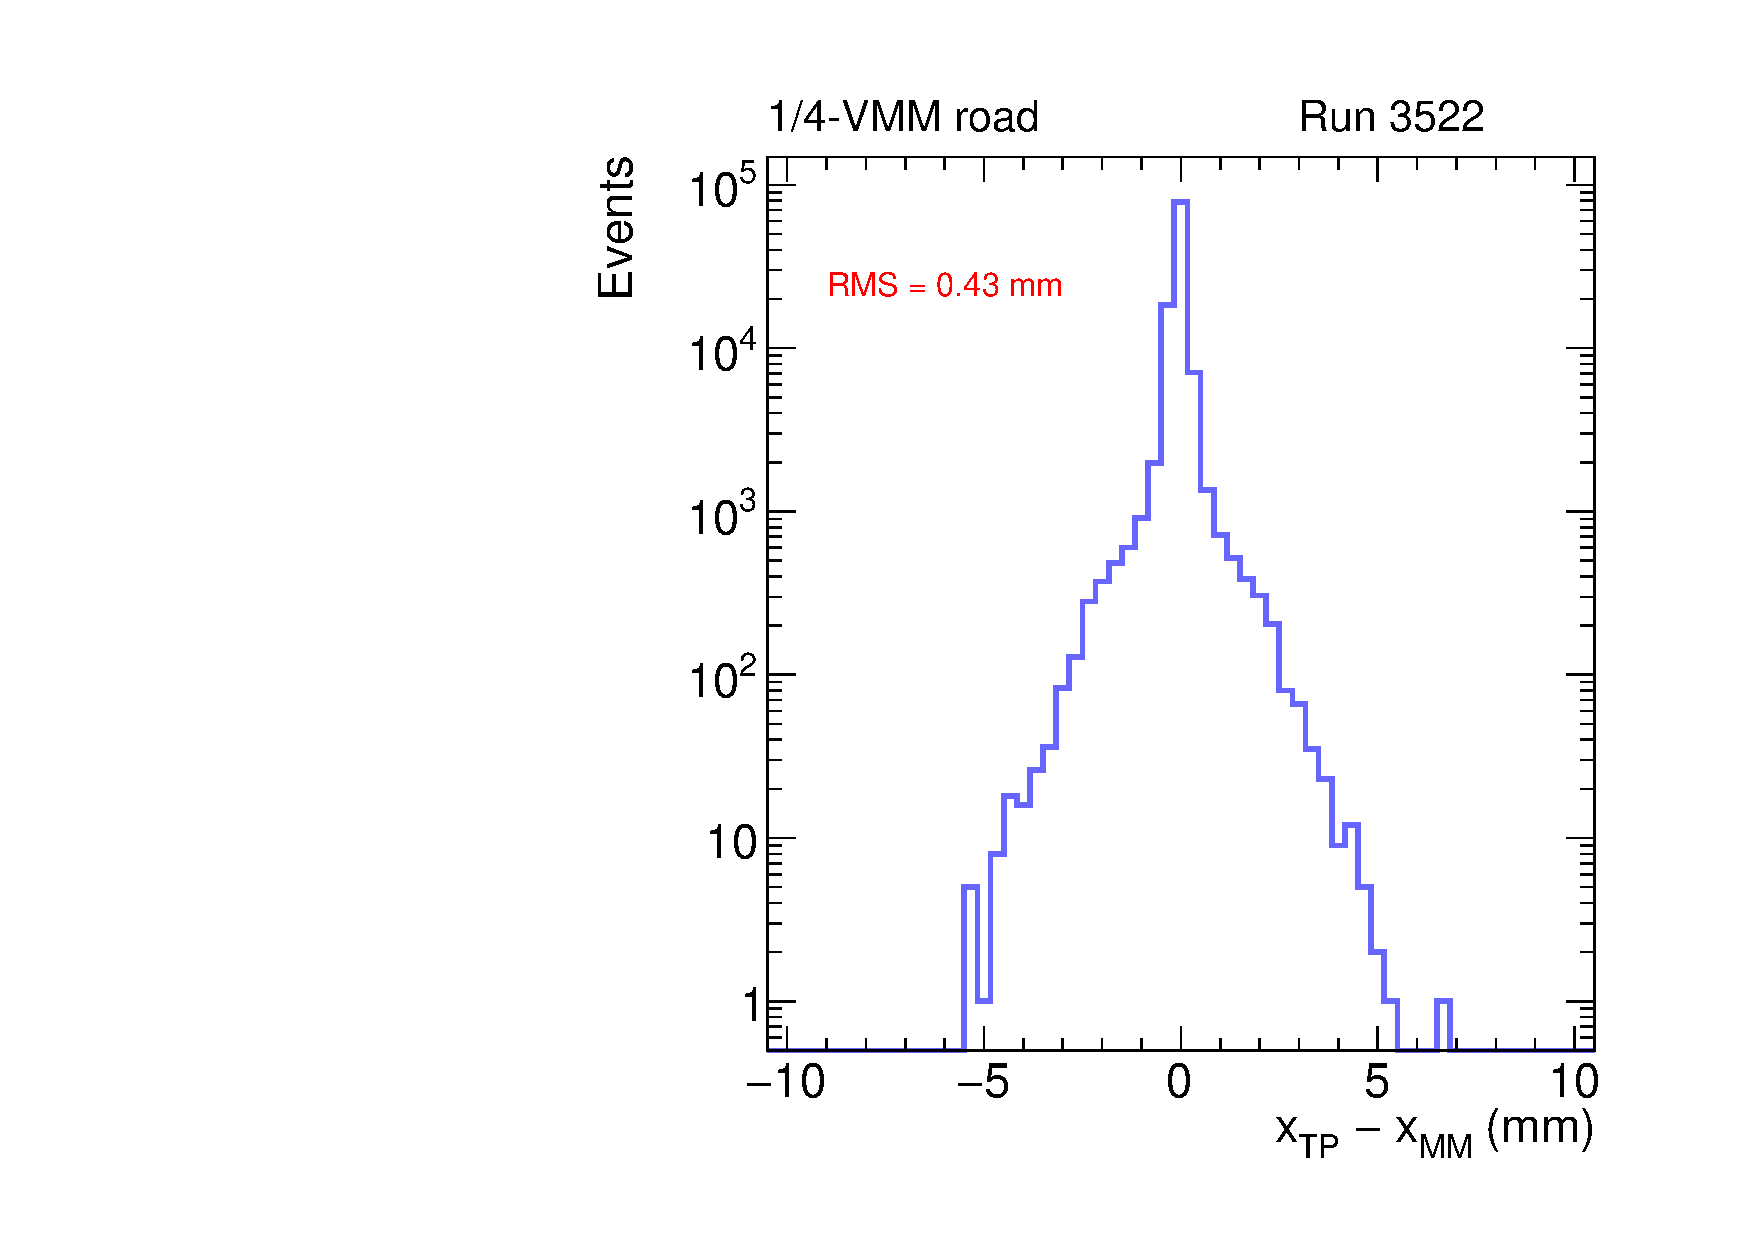
\includegraphics[width=0.4\textwidth]{figures/gbtanalysis3522/TP_xres.pdf}
  \end{center}
  \vspace{-10pt}
  \caption{The $x$ resolution of the MM TP relative to the full readout, using 1-VMM online roads (left) and 1/4-VMM offline roads (right). The tails of the resolution are greatly suppressed with smaller roads.}
  \label{fig:xres}
\end{figure}

\begin{figure}[!htpb]
  \begin{center}
    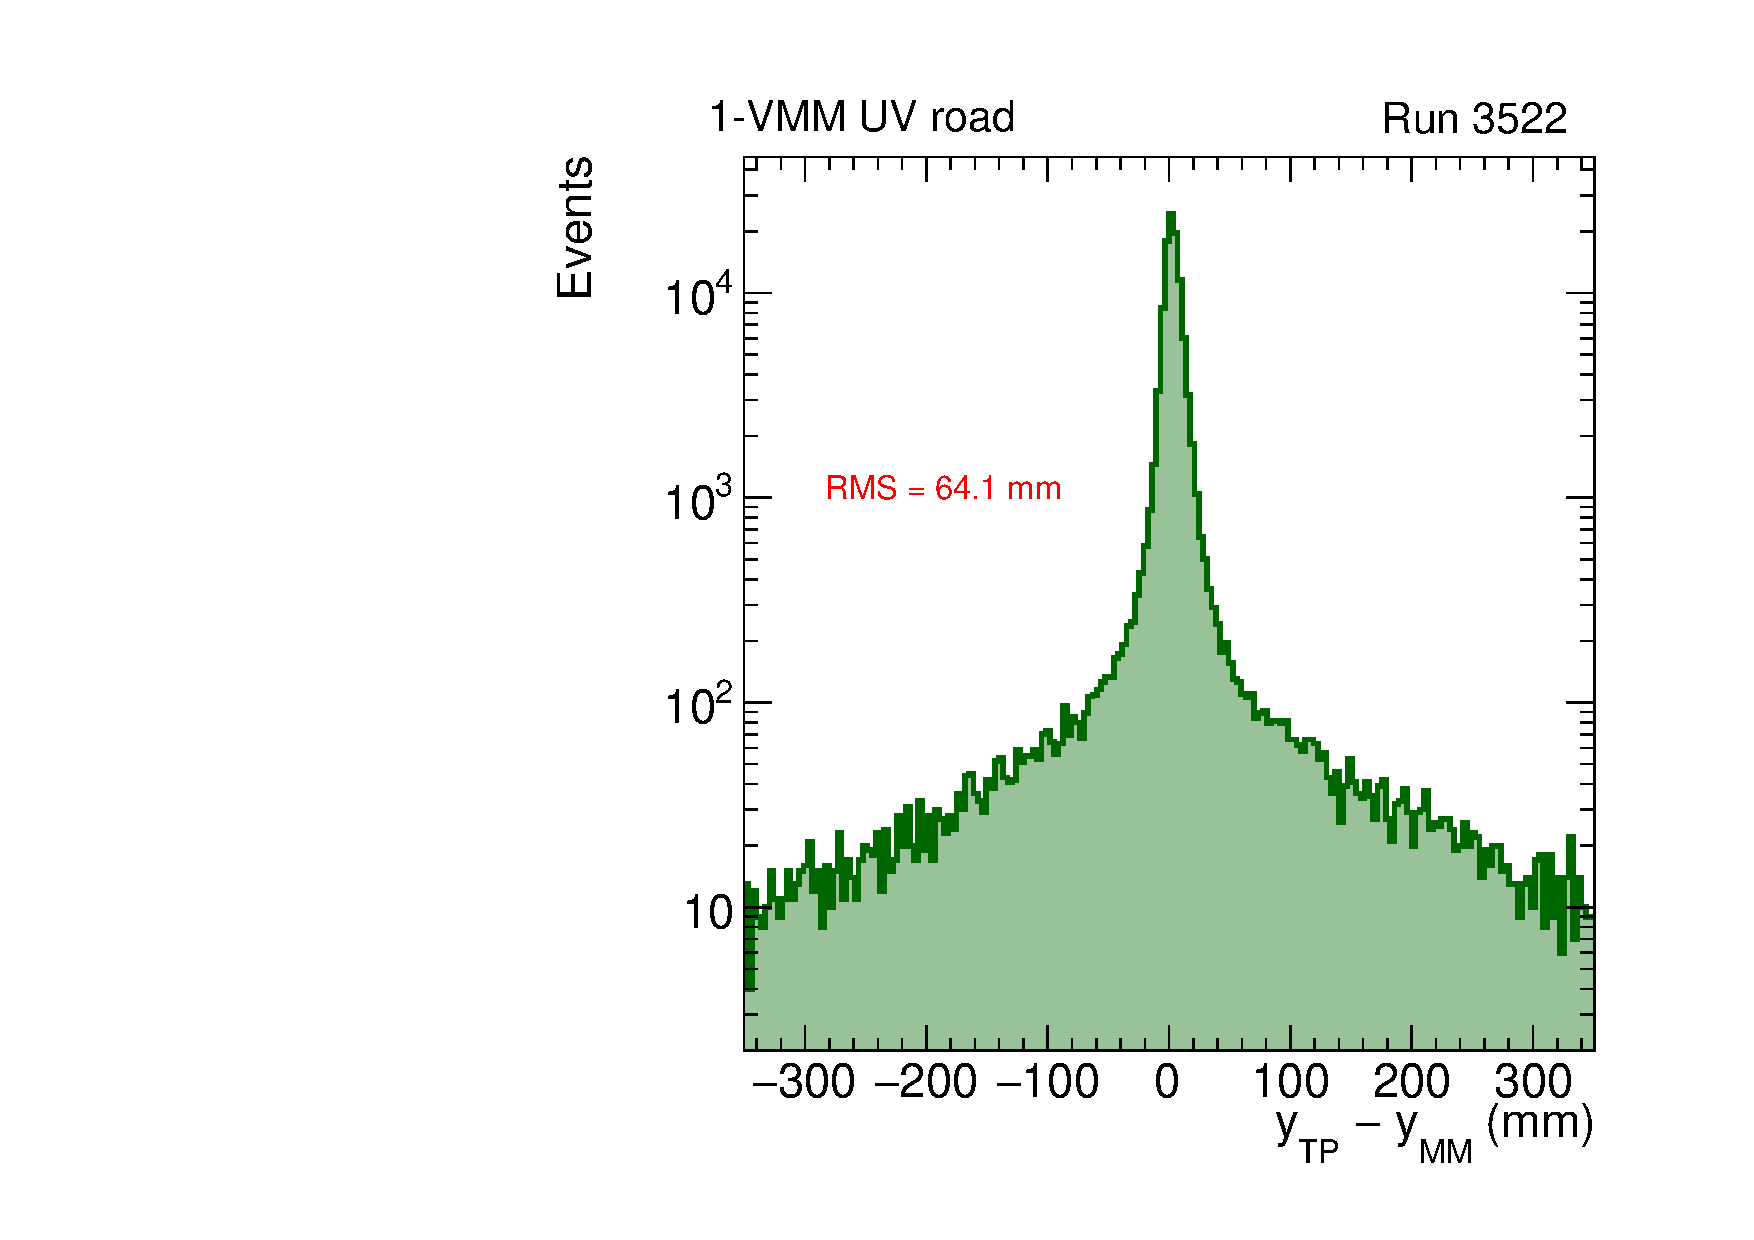
\includegraphics[width=0.4\textwidth]{figures/gbtanalysis3522/TP_yres_1road.pdf}
    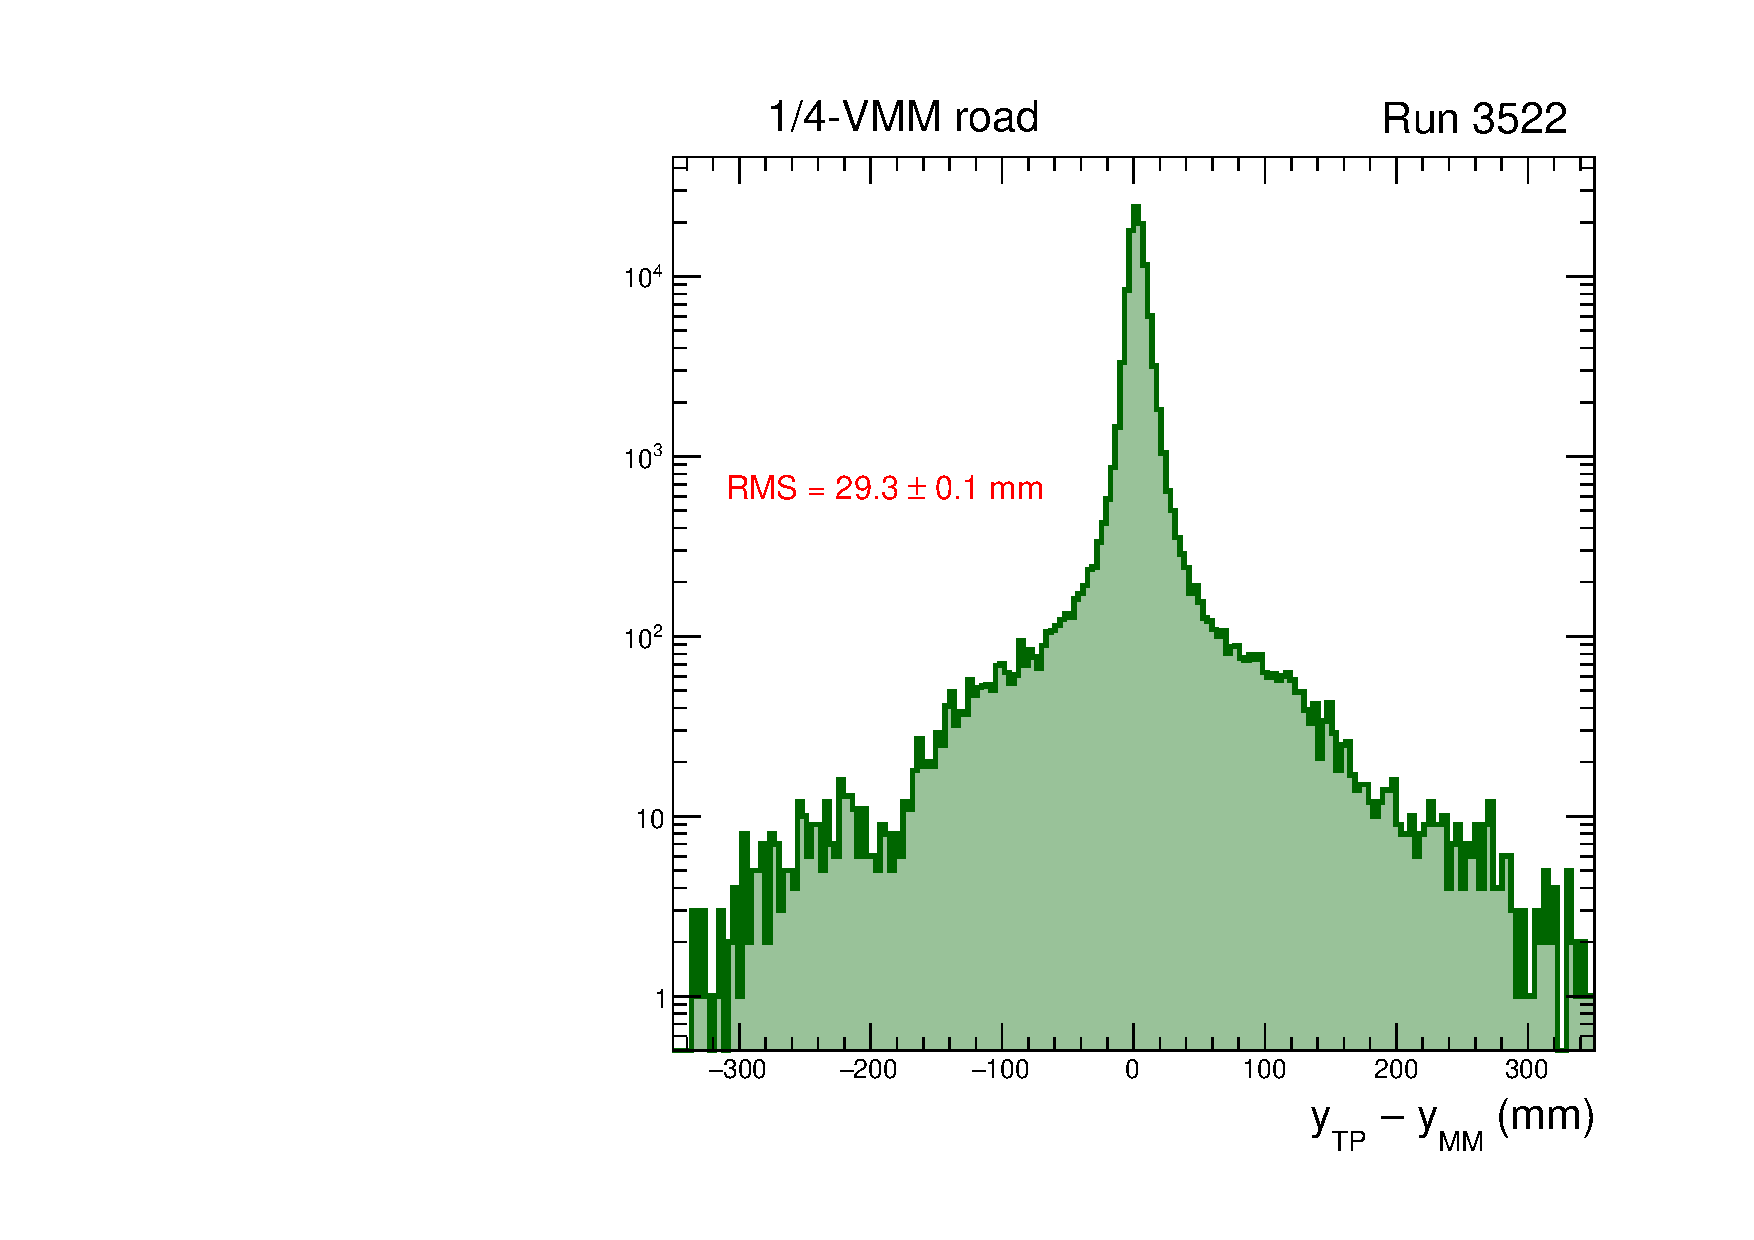
\includegraphics[width=0.4\textwidth]{figures/gbtanalysis3522/TP_yres_smallroad.pdf}
  \end{center}
  \vspace{-10pt}
  \caption{The $y$ resolution of the MM TP relative to the full readout, using 1-VMM online roads (left) and 1/4-VMM offline roads (right). The tails of the resolution are greatly suppressed with smaller roads.}
  \label{fig:yres}
\end{figure}

\begin{figure}[!htpb]
  \begin{center}
    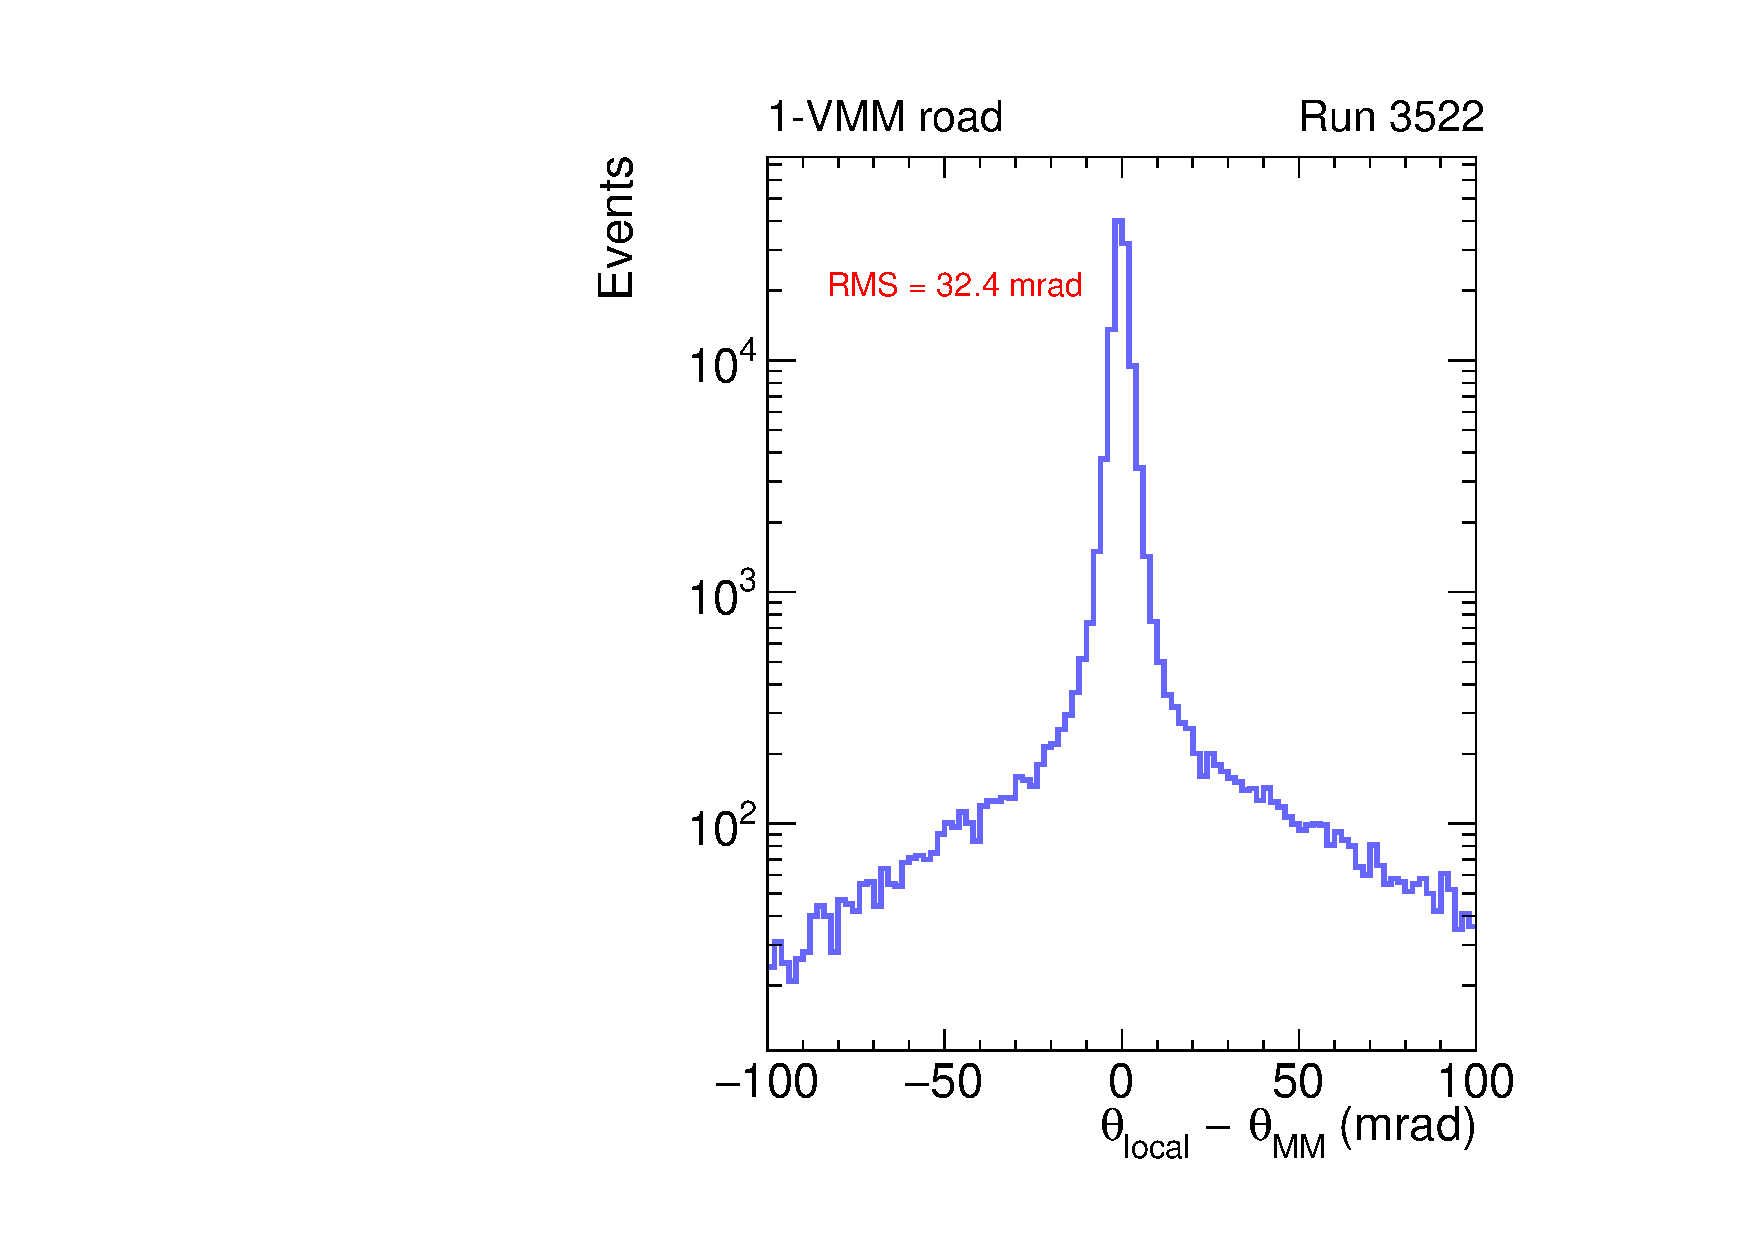
\includegraphics[width=0.4\textwidth]{figures/gbtanalysis3522/TP_angres_full.pdf}
    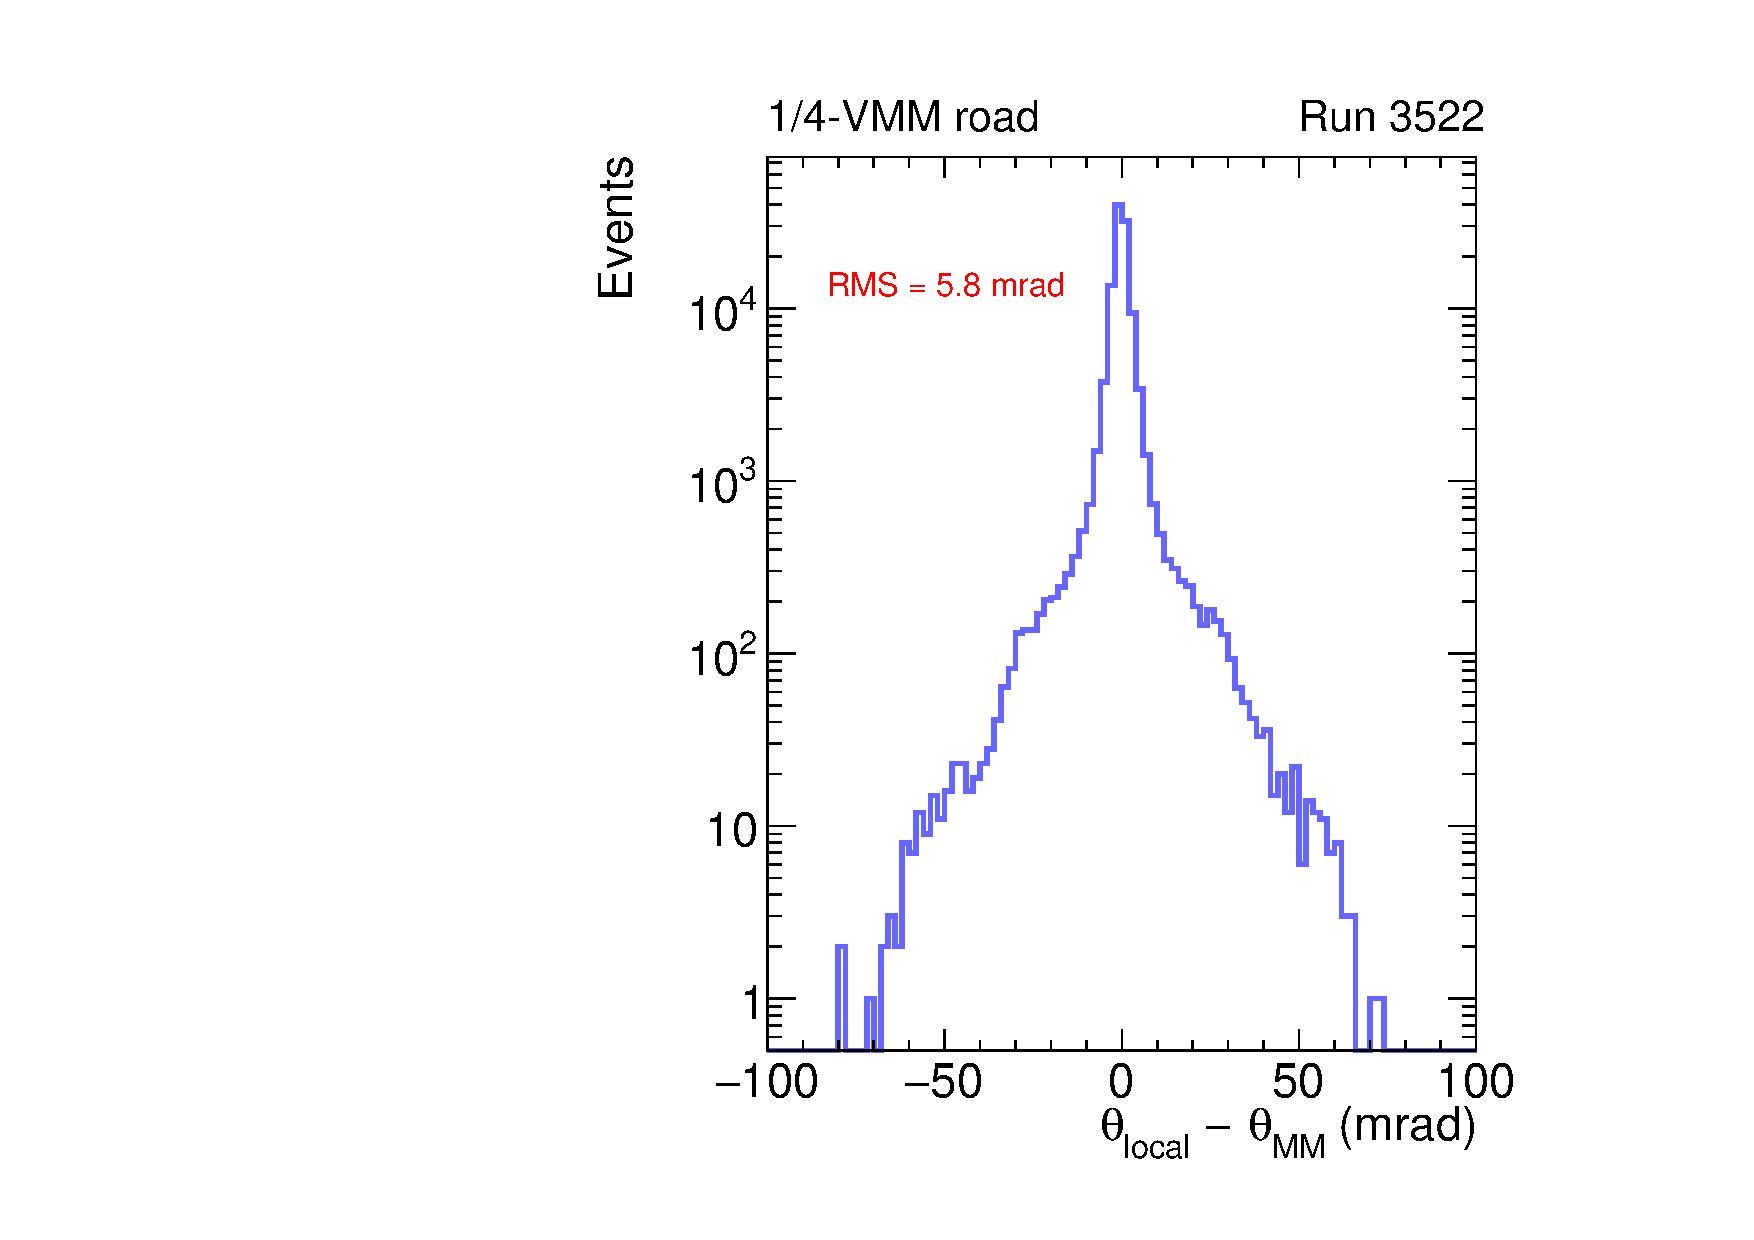
\includegraphics[width=0.4\textwidth]{figures/gbtanalysis3522/TP_angres.pdf}
  \end{center}
  \vspace{-10pt}
  \caption{The $\theta$ resolution of the MM TP relative to the full readout, using 1-VMM online roads (left) and 1/4-VMM offline roads (right). The tails of the resolution are greatly suppressed with smaller roads.}
  \label{fig:thetares}
\end{figure}

\begin{figure}[!htpb]
  \begin{center}
    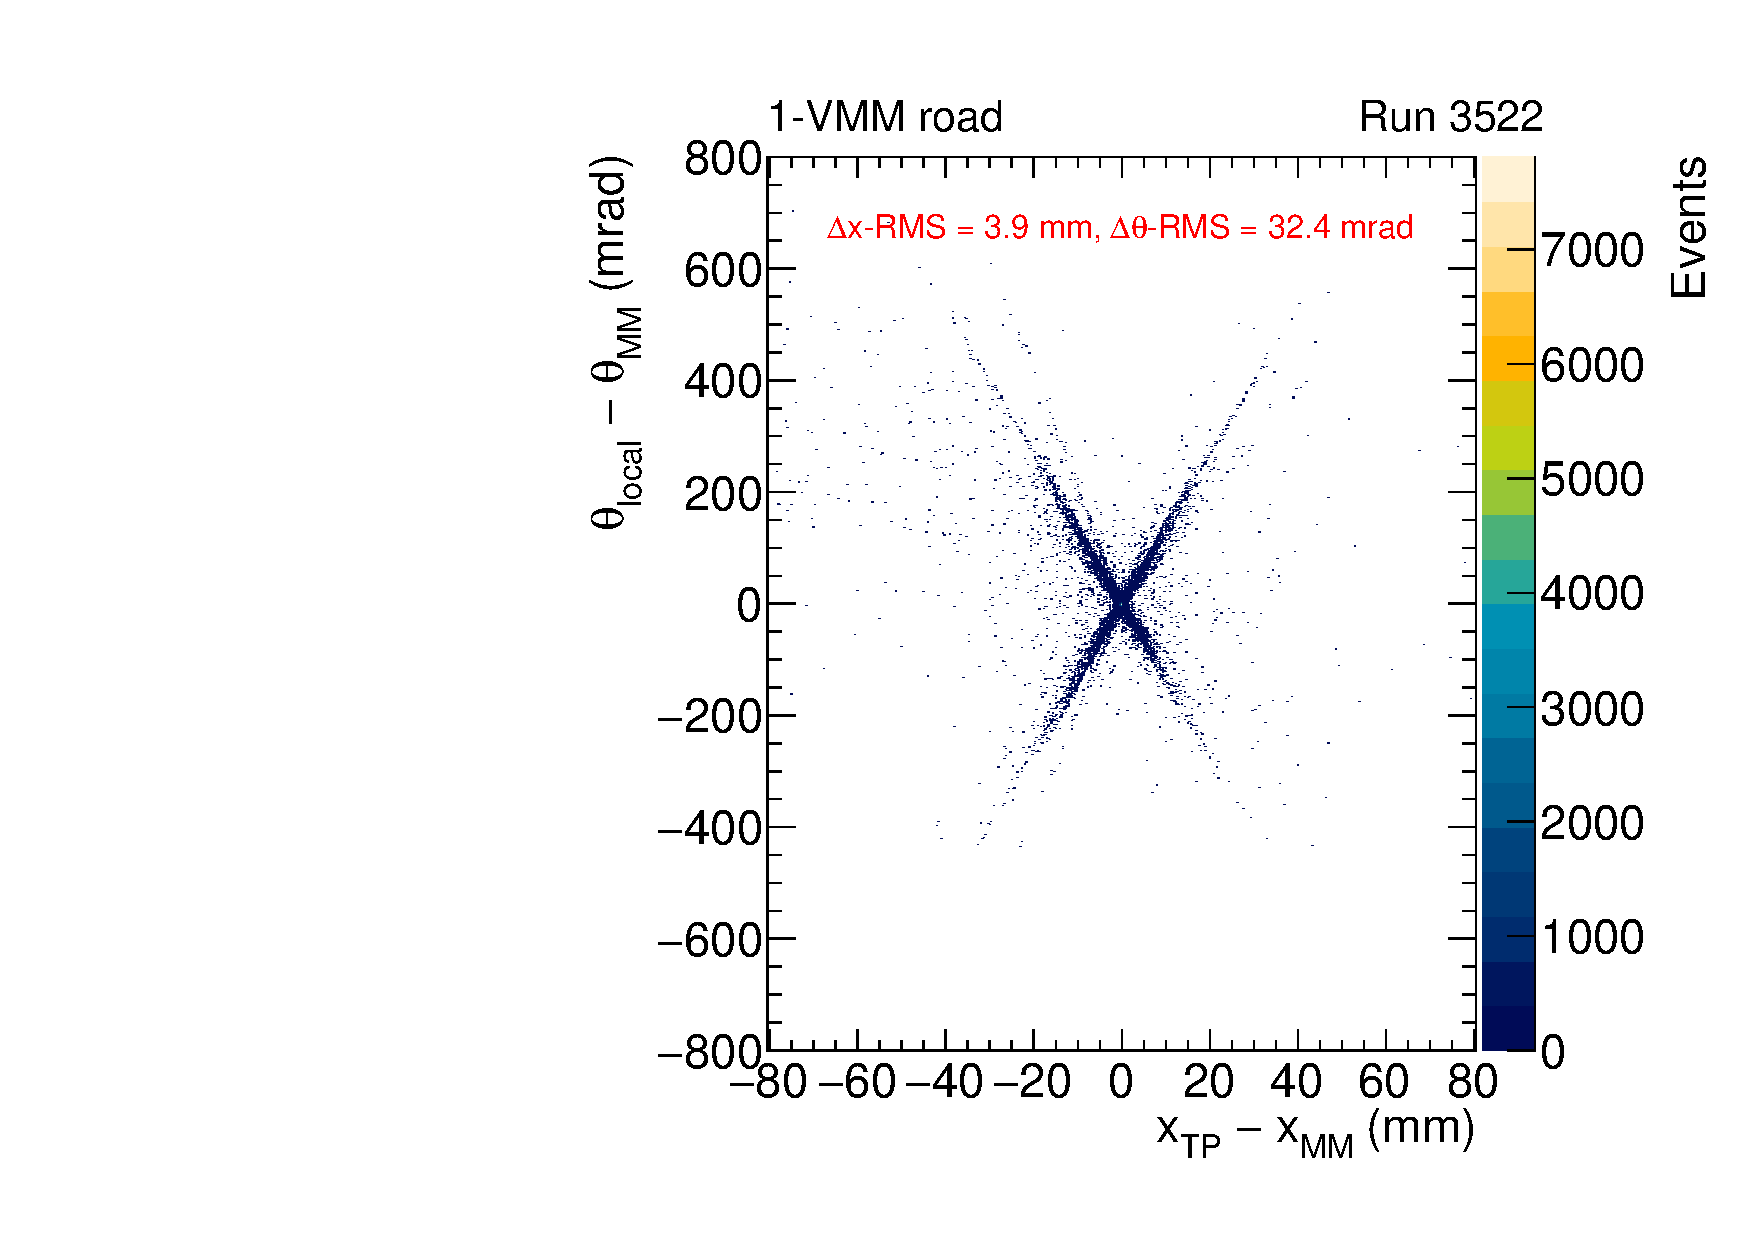
\includegraphics[width=0.4\textwidth]{figures/gbtanalysis3522/TP_xres_angres_full.pdf}
    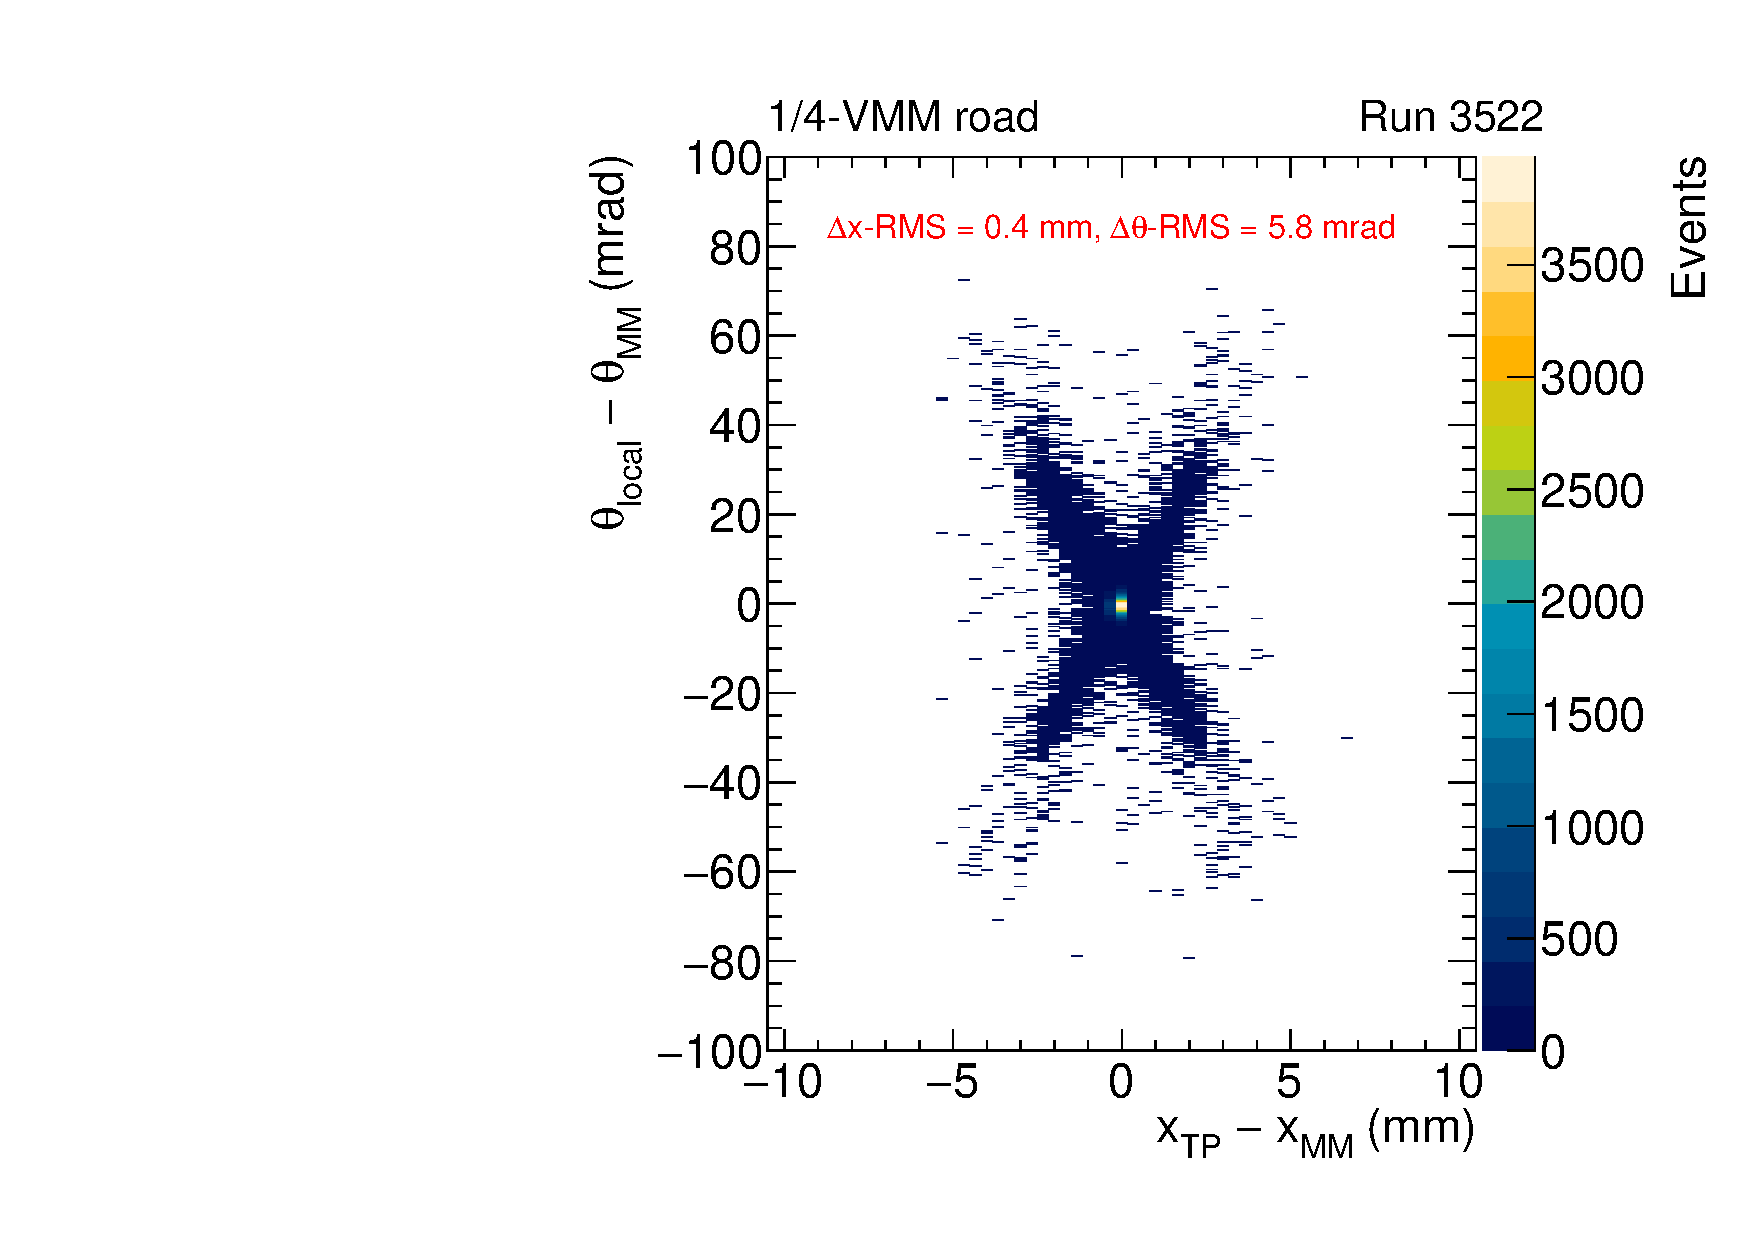
\includegraphics[width=0.4\textwidth]{figures/gbtanalysis3522/TP_xres_angres.pdf}
  \end{center}
  \vspace{-10pt}
  \caption{The $x$ and $\theta$ resolution of the MM TP relative to the full readout, using 1-VMM online roads (left) and 1/4-VMM offline roads (right). The tails of the resolution are greatly suppressed with smaller roads.}
  \label{fig:xthetares}
\end{figure}

\begin{figure}[!htpb]
  \begin{center}
    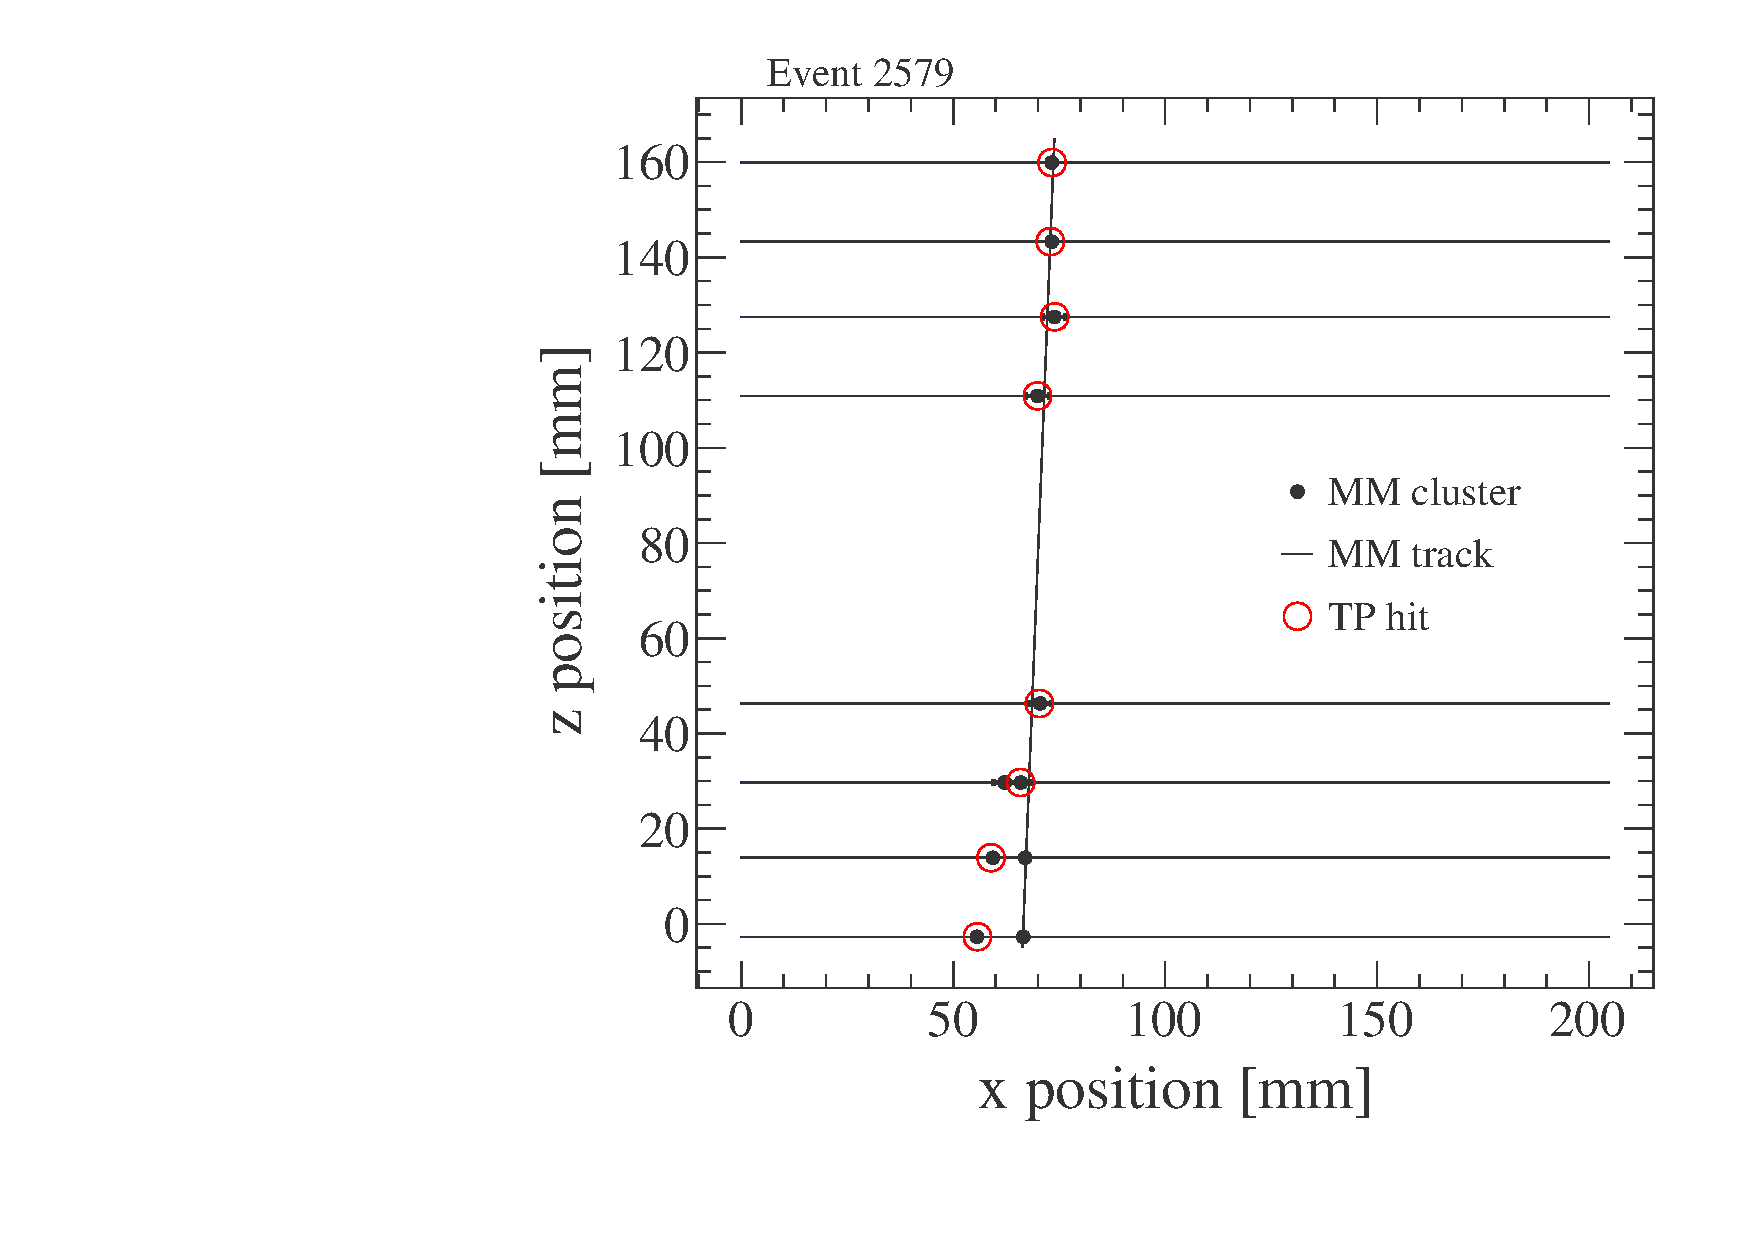
\includegraphics[width=0.4\textwidth]{figures/event_displays/display_02579.pdf}
    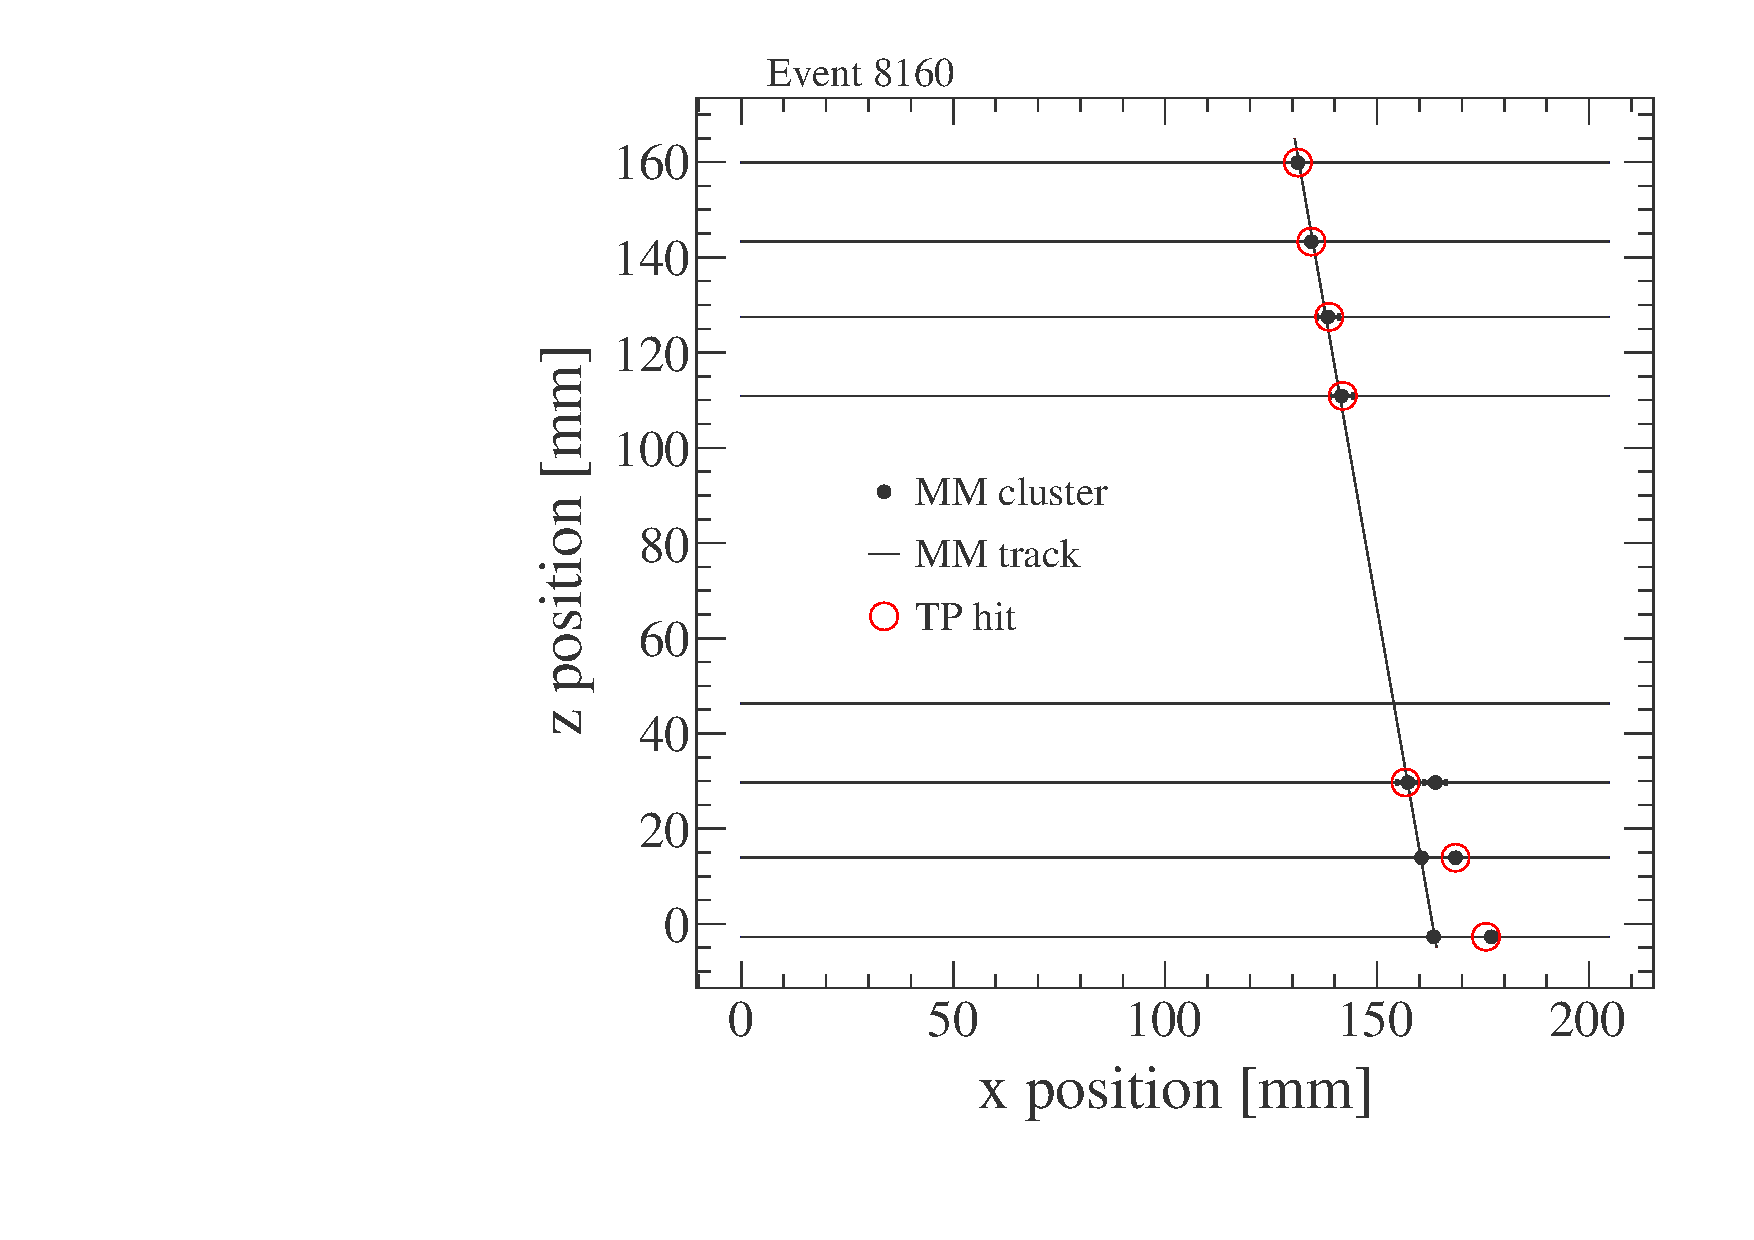
\includegraphics[width=0.4\textwidth]{figures/event_displays/display_08160.pdf}
  \end{center}
  \vspace{-10pt}
  \caption{Two event displays likely to include delta rays. The black circles are clusters from the full MMFE8 readout, the black line is the fit to the clusters, and the red circles are the hits chosen by the MM TP. In both cases, the MM TP chooses hits from the delta ray.}
  \label{fig:deltarays}
\end{figure}


\subsection{Time resolution}

\begin{figure}[!htpb]
  \begin{center}
    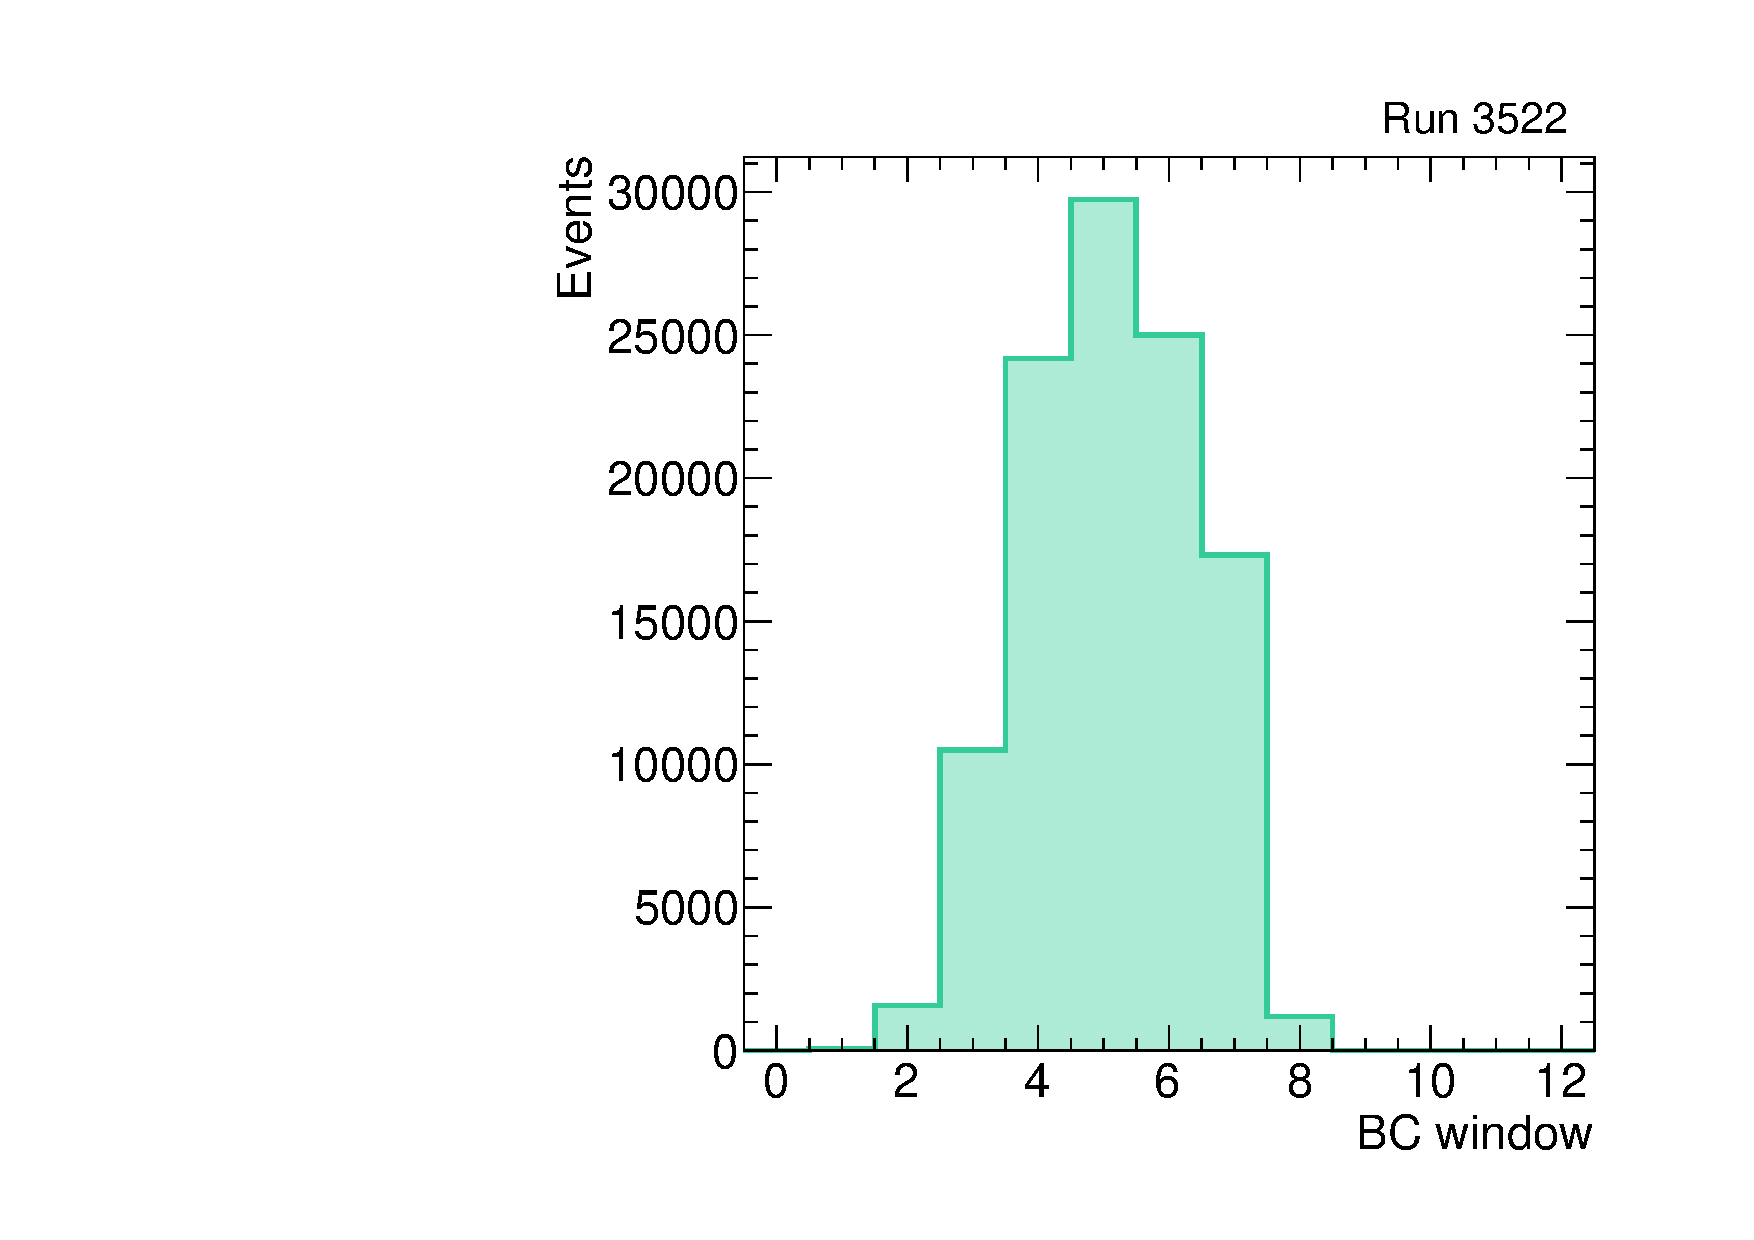
\includegraphics[width=0.4\textwidth]{figures/gbtanalysis3522/artwin_lin.pdf}
    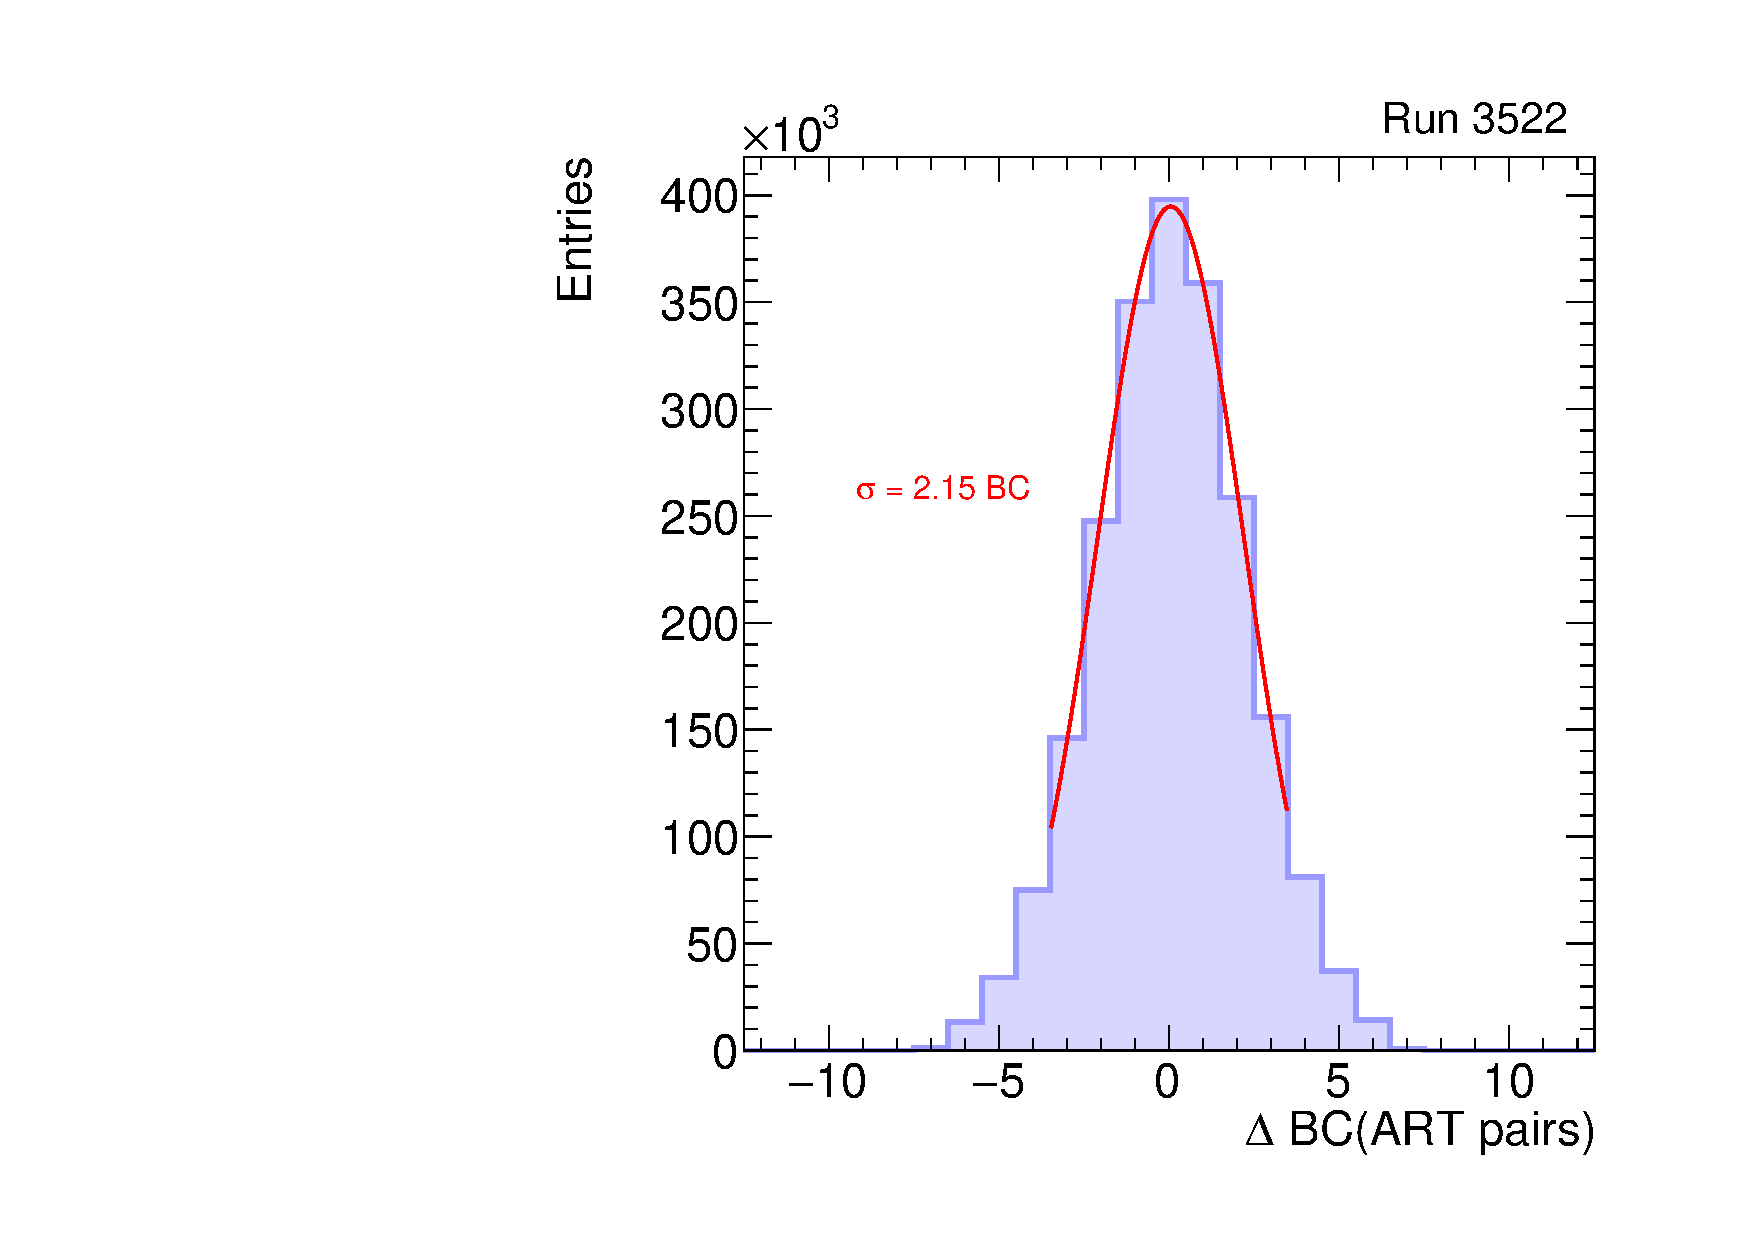
\includegraphics[width=0.4\textwidth]{figures/gbtanalysis3522/artrpairs_lin.pdf}
  \end{center}
  \vspace{-10pt}
  \caption{The time window required to record all hits in a trigger (left) and the $\Delta\text{BC}$ of all pairs of hits in a trigger (right). A gaussian fit is overlaid on the distribution of $\Delta\text{BC}$ and describes the data well.}
  \label{fig:time}
\end{figure}

\begin{figure}[!htpb]
  \begin{center}
    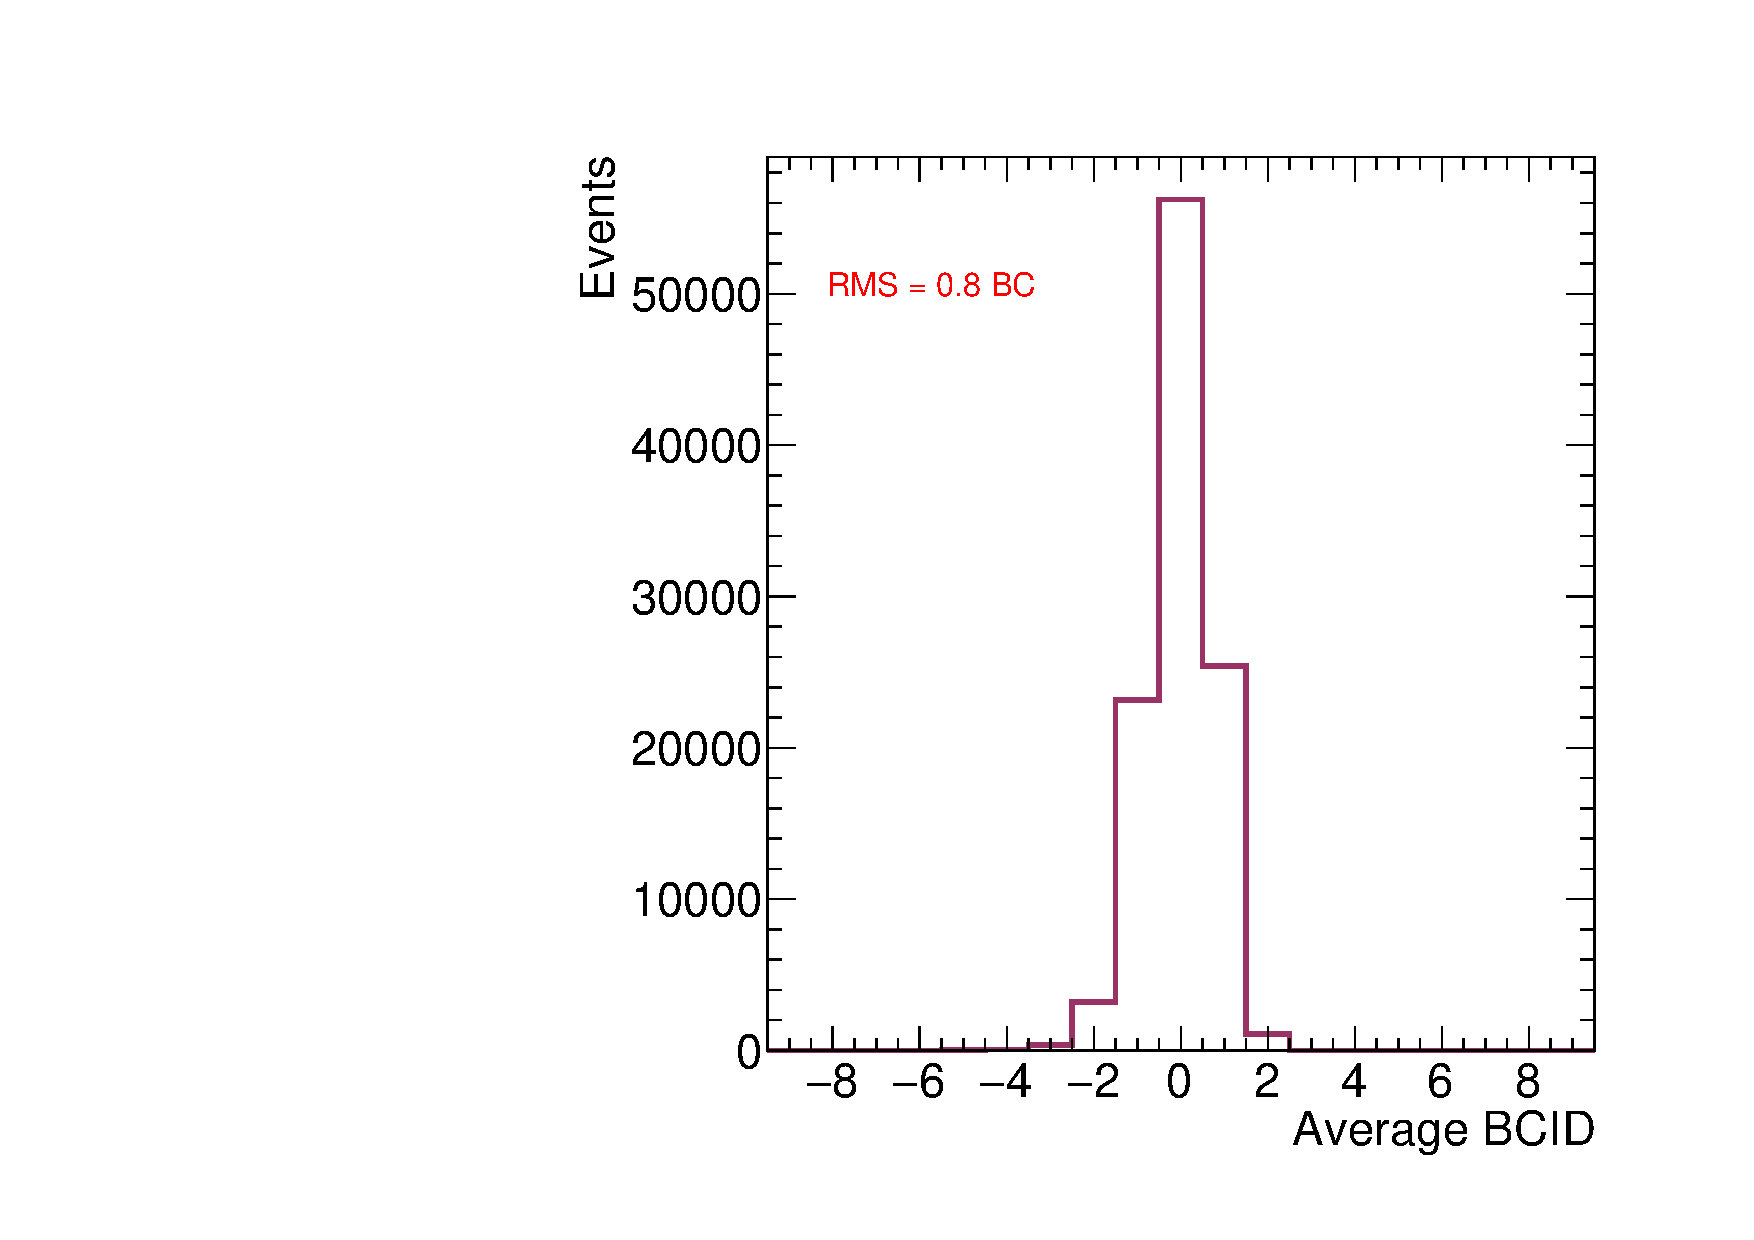
\includegraphics[width=0.4\textwidth]{figures/gbtanalysis3522/avg_BCID.pdf}
    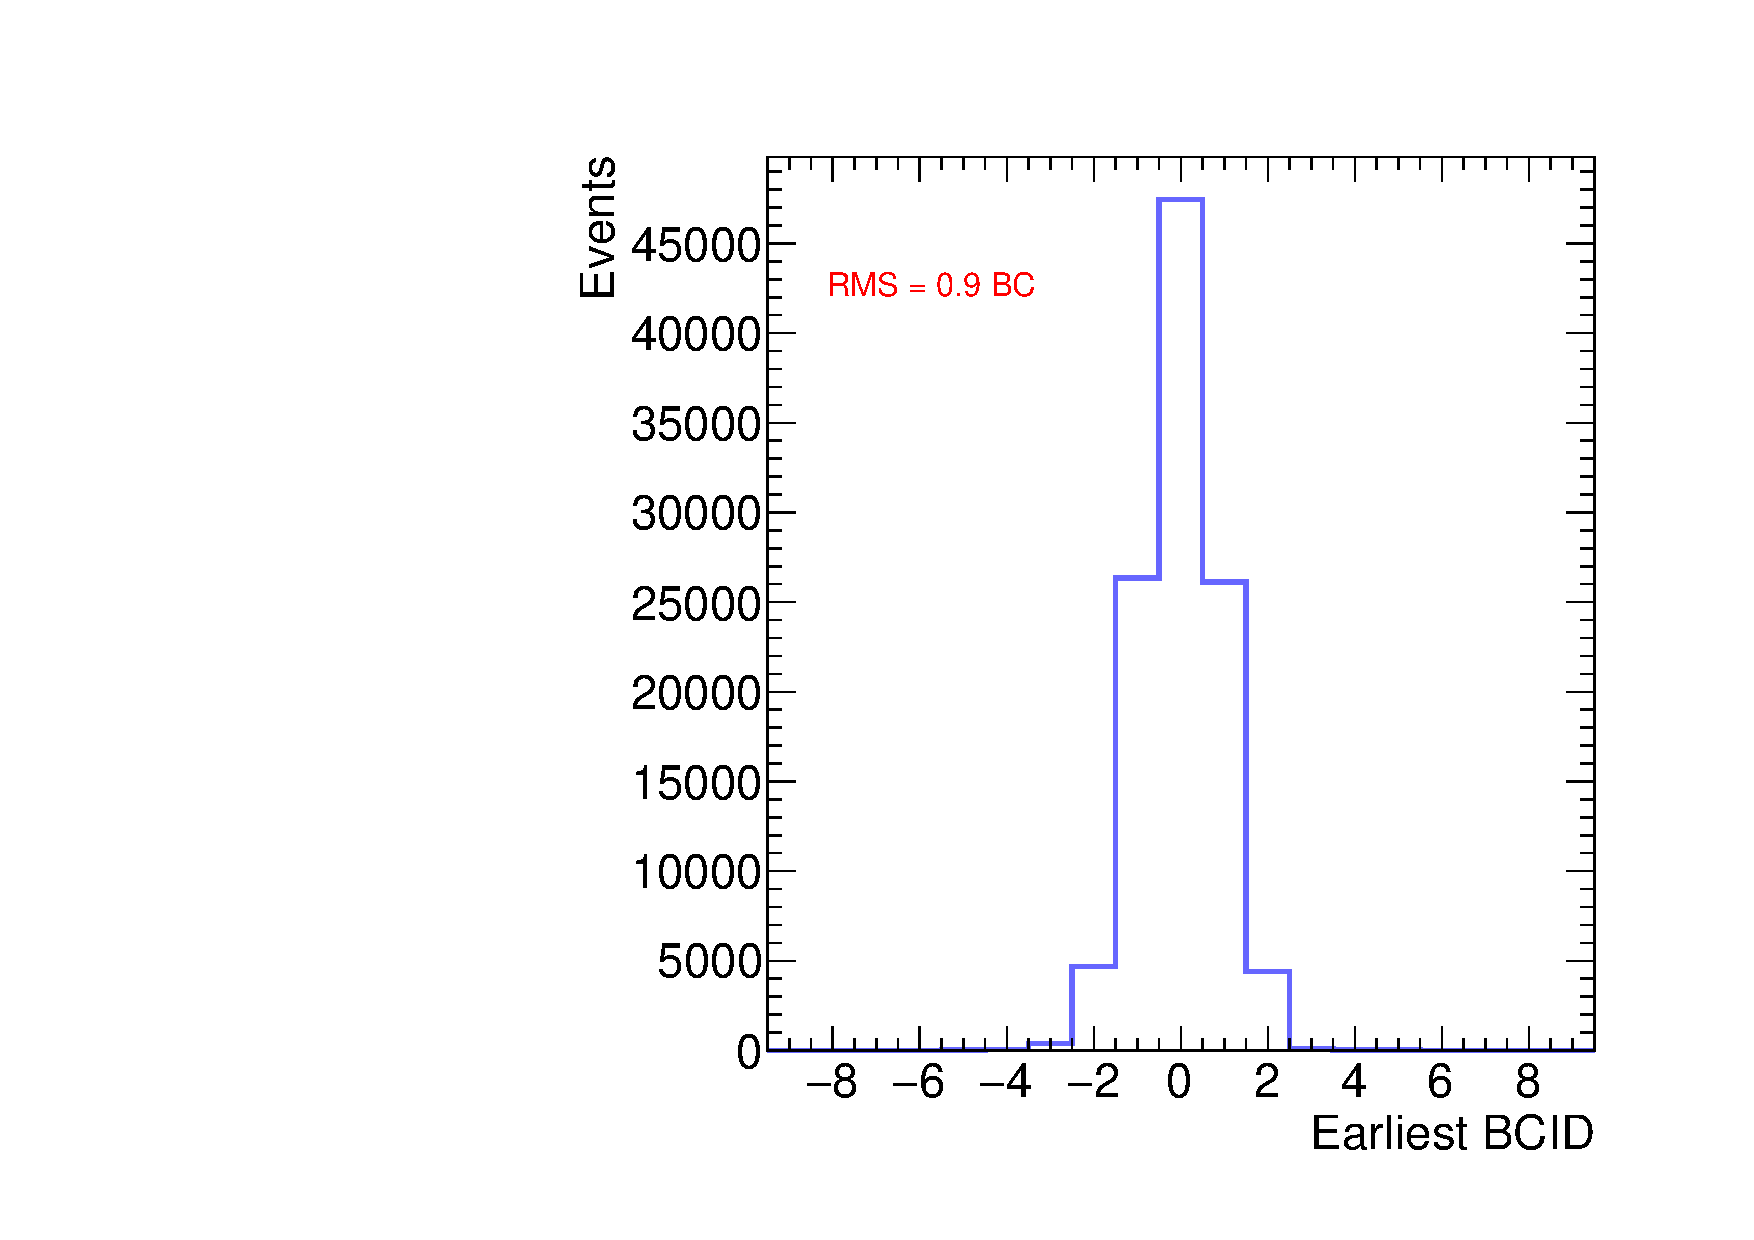
\includegraphics[width=0.4\textwidth]{figures/gbtanalysis3522/earliest_BCID.pdf}
  \end{center}
  \vspace{-10pt}
  \caption{The time resolution of the MM TP relative to the scintillator. The BCID of the trigger can be defined as the average BCID of the ART hits (left) or the earliest BCID (right). Choosing the average BCID has better resolution than choosing the earliest.}
  \label{fig:timeres}
\end{figure}

\subsection{Integration time}
\label{sec:perf-integ}

\begin{figure}[!htpb]
  \begin{center}
    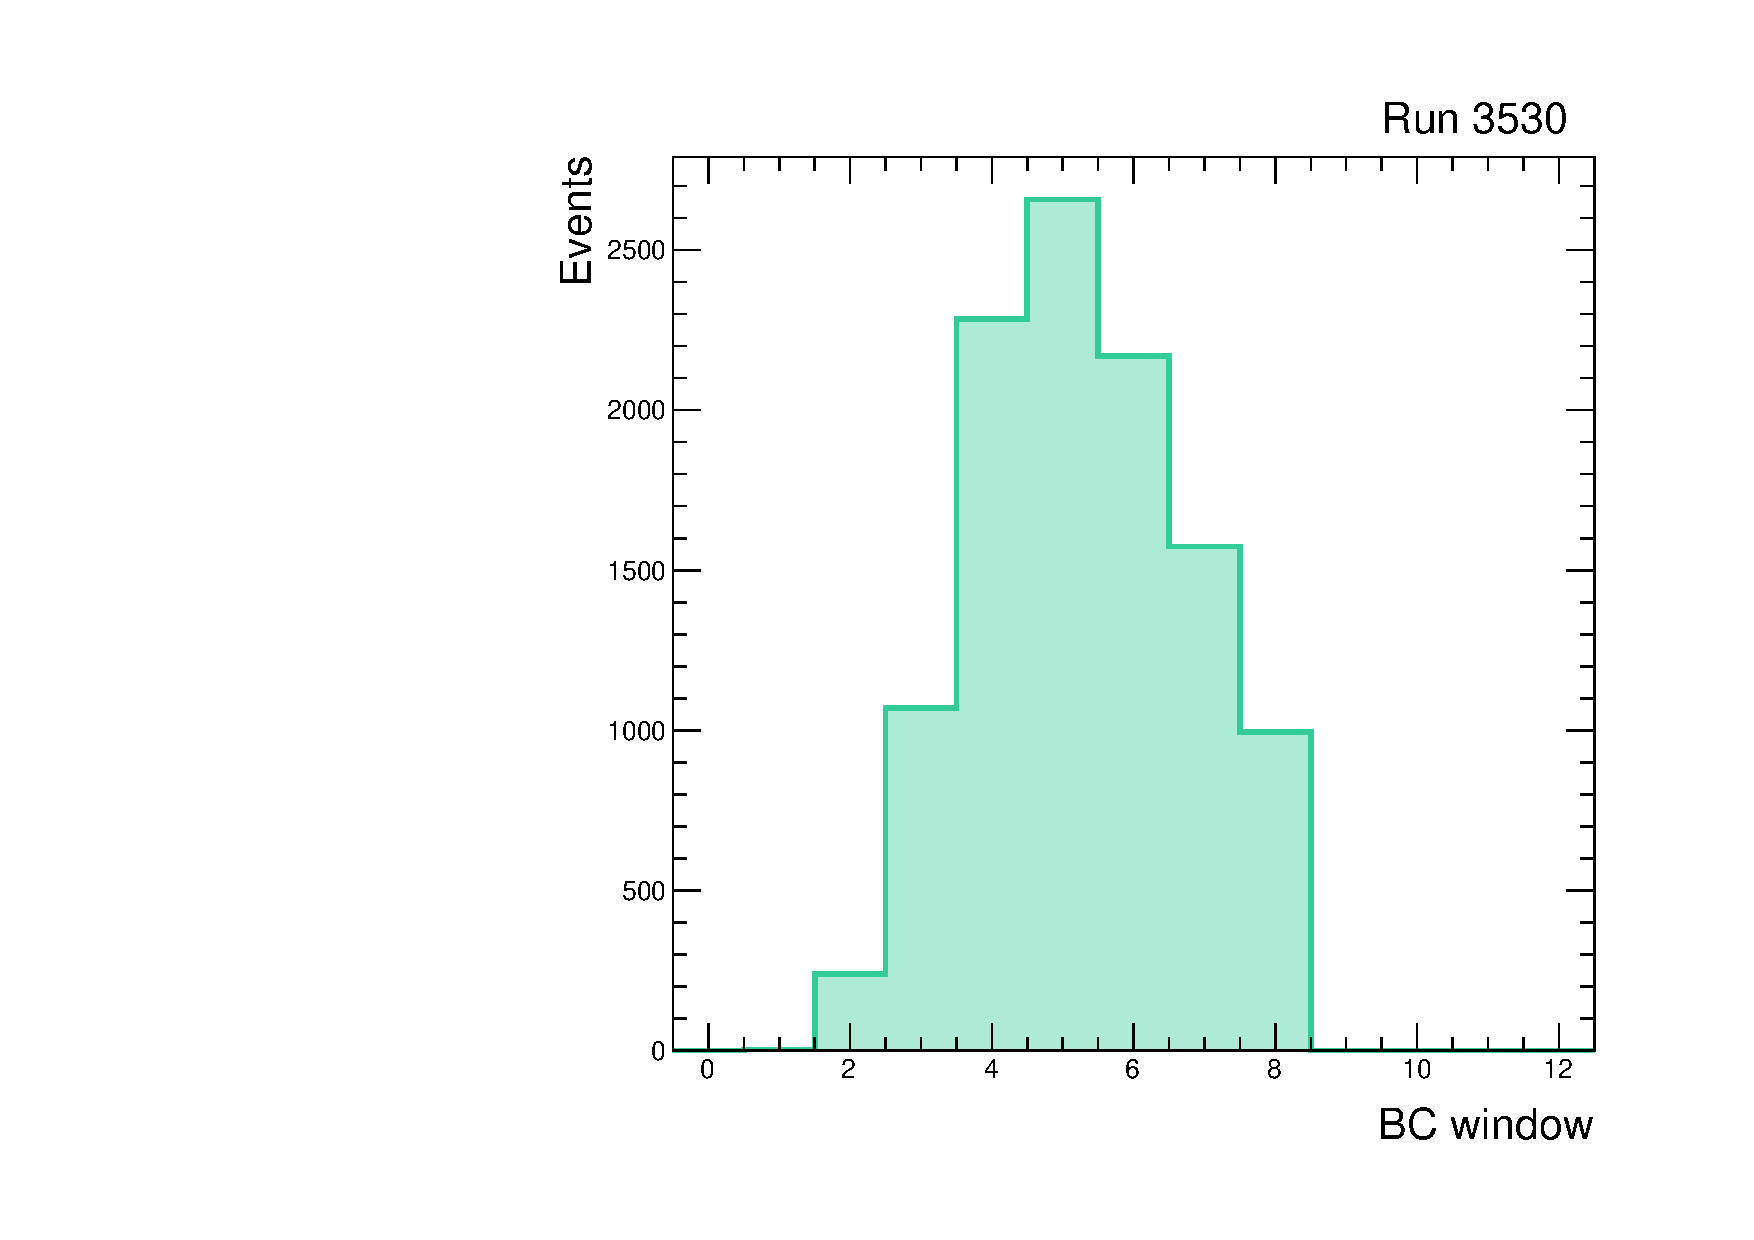
\includegraphics[width=0.3\textwidth]{figures/gbtanalysis3530/artwin_lin.pdf}
    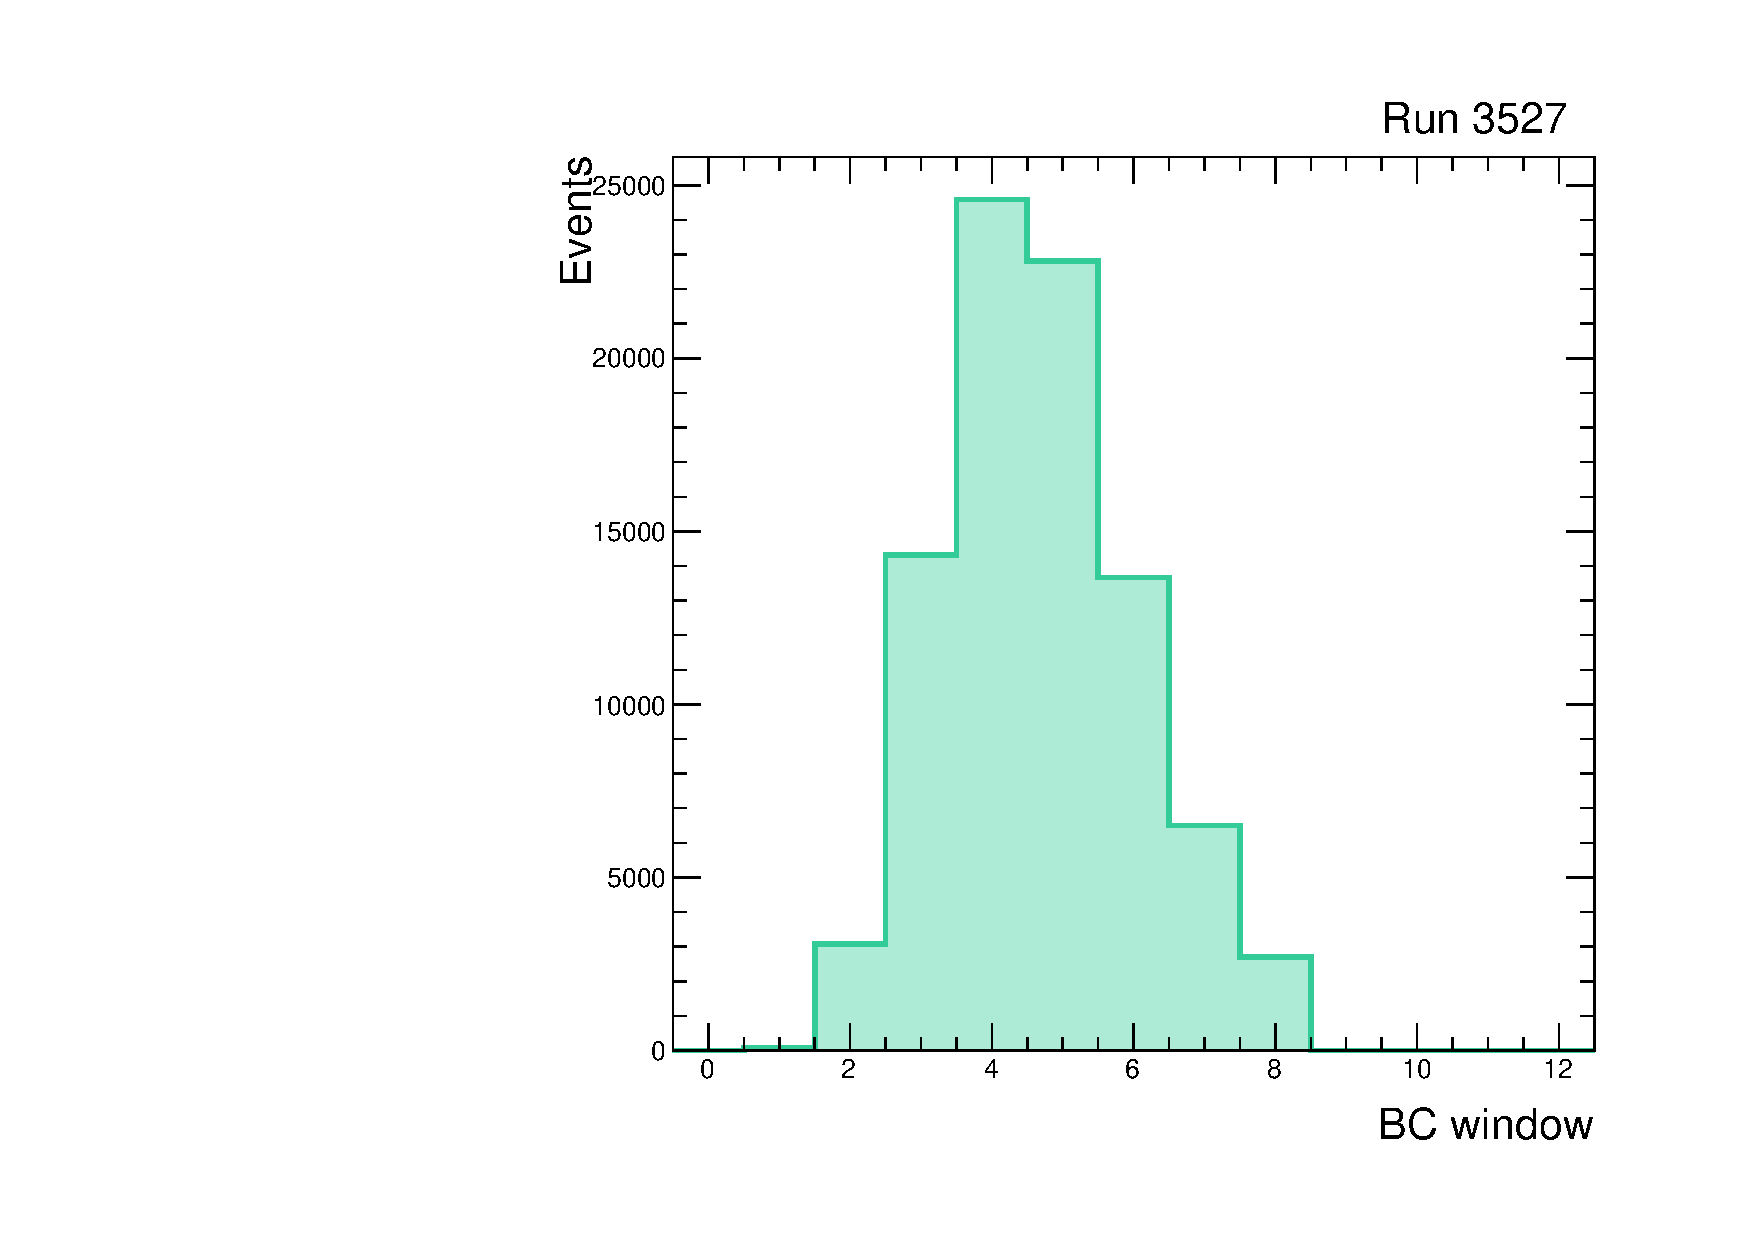
\includegraphics[width=0.3\textwidth]{figures/gbtanalysis3527/artwin_lin.pdf}
    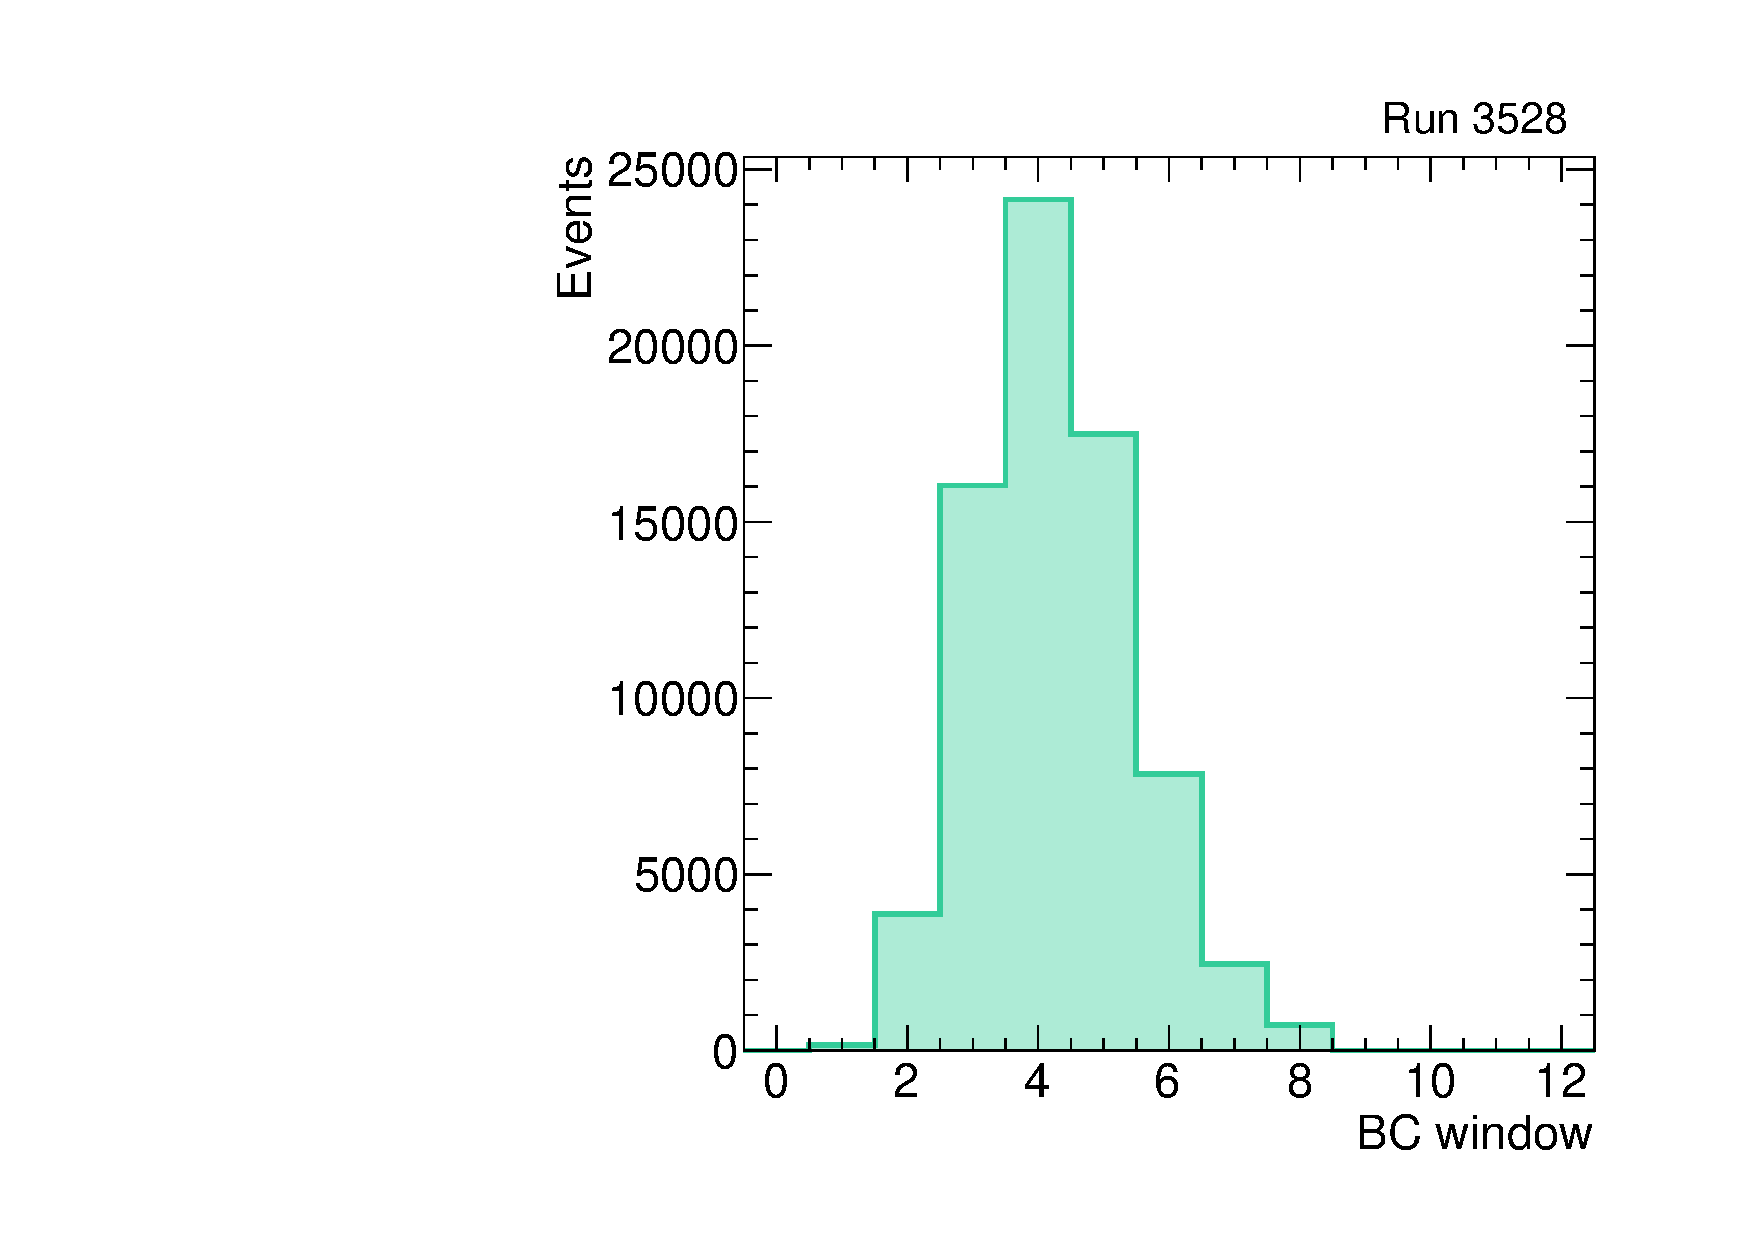
\includegraphics[width=0.3\textwidth]{figures/gbtanalysis3528/artwin_lin.pdf}
  \end{center}
  \vspace{-10pt}
  \caption{The time window required to record all hits in a trigger for data collected with 200 ns (left), 100 ns (middle), and 50 ns (right) integration time in the VMM. The window decreases as the integration time decreases.}
  \label{fig:integ_window}
\end{figure}

\begin{figure}[!htpb]
  \begin{center}
    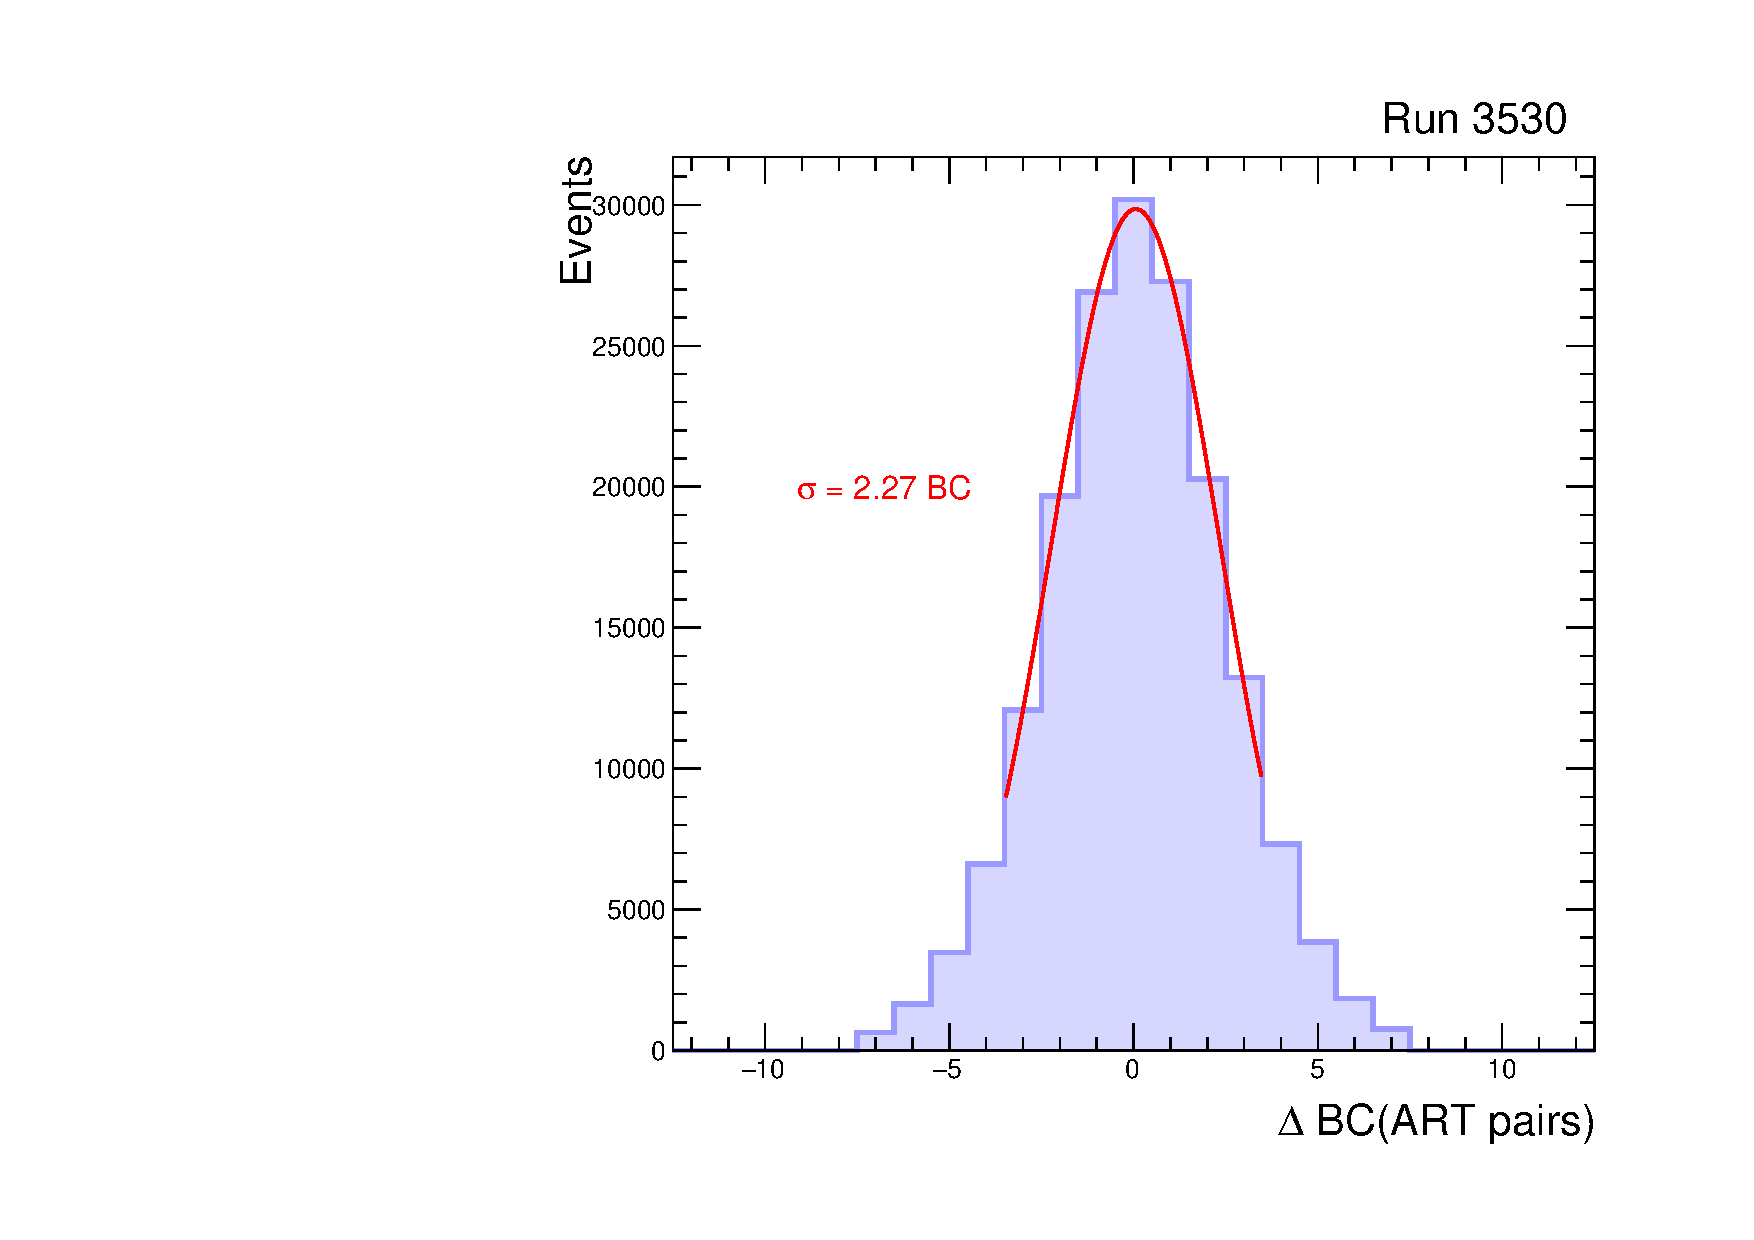
\includegraphics[width=0.3\textwidth]{figures/gbtanalysis3530/artrpairs_lin.pdf}
    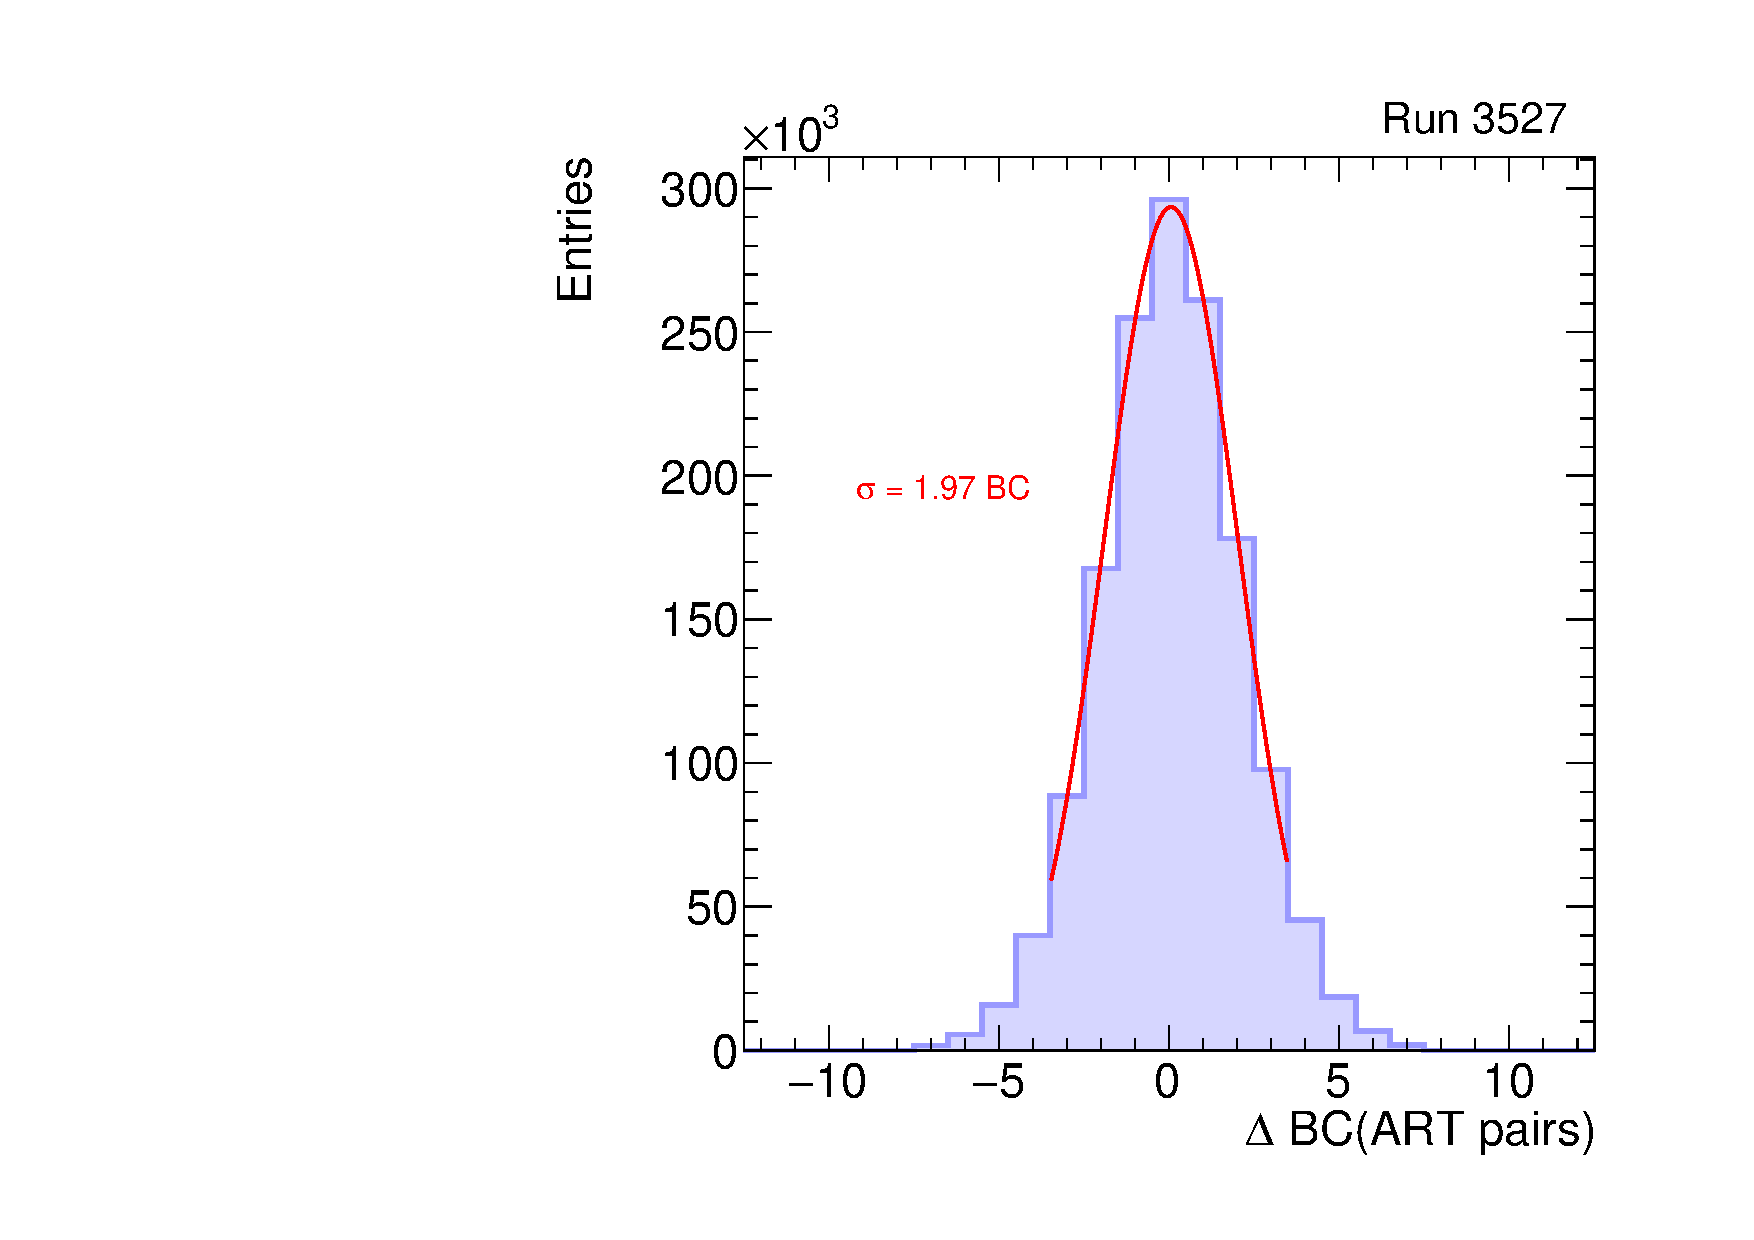
\includegraphics[width=0.3\textwidth]{figures/gbtanalysis3527/artrpairs_lin.pdf}
    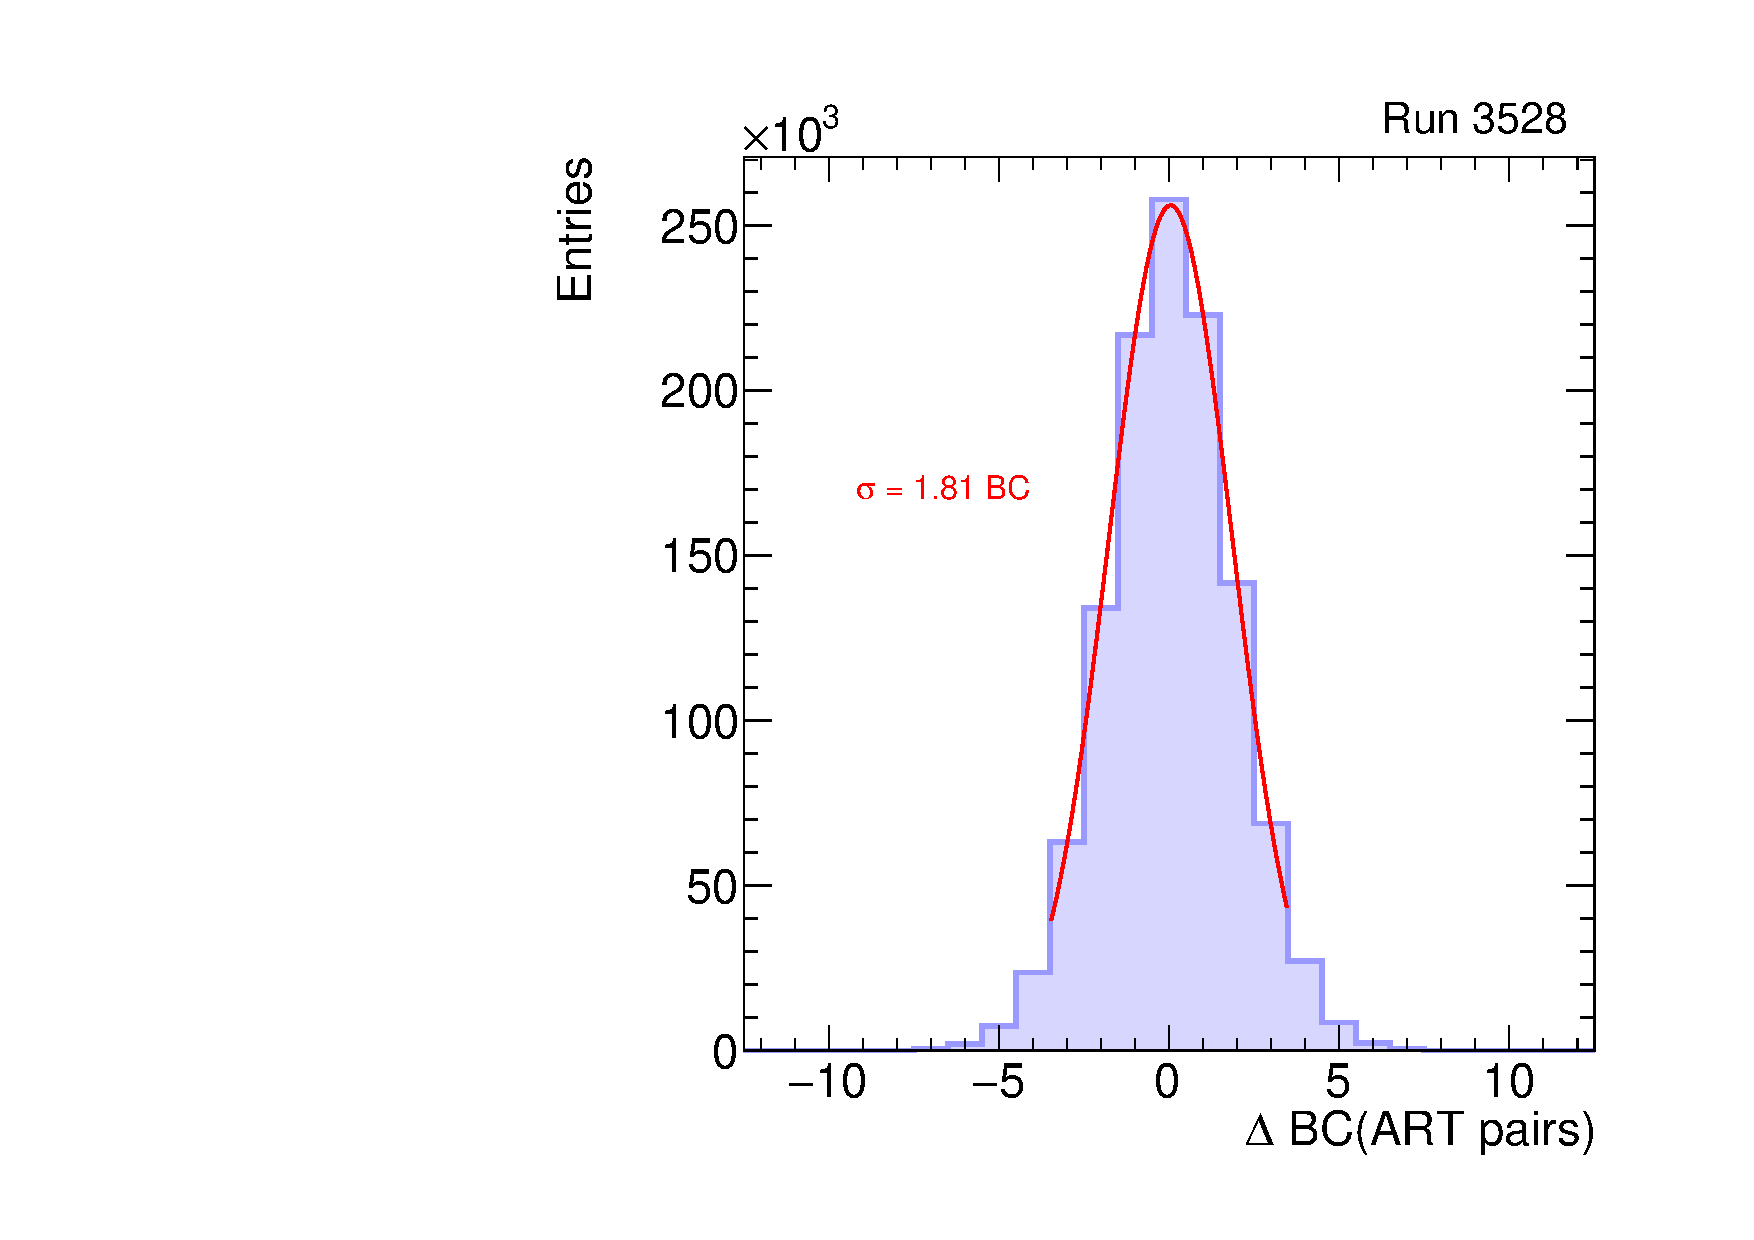
\includegraphics[width=0.3\textwidth]{figures/gbtanalysis3528/artrpairs_lin.pdf}
  \end{center}
  \vspace{-10pt}
  \caption{The $\Delta\text{BC}$ of all pairs of hits in a trigger for data collected with 200 ns (left), 100 ns (middle), and 50 ns (right) integration time in the VMM. The distribution is narrower as the integration time decreases.}
  \label{fig:integ_pairs}
\end{figure}

\begin{figure}[!htpb]
  \begin{center}
    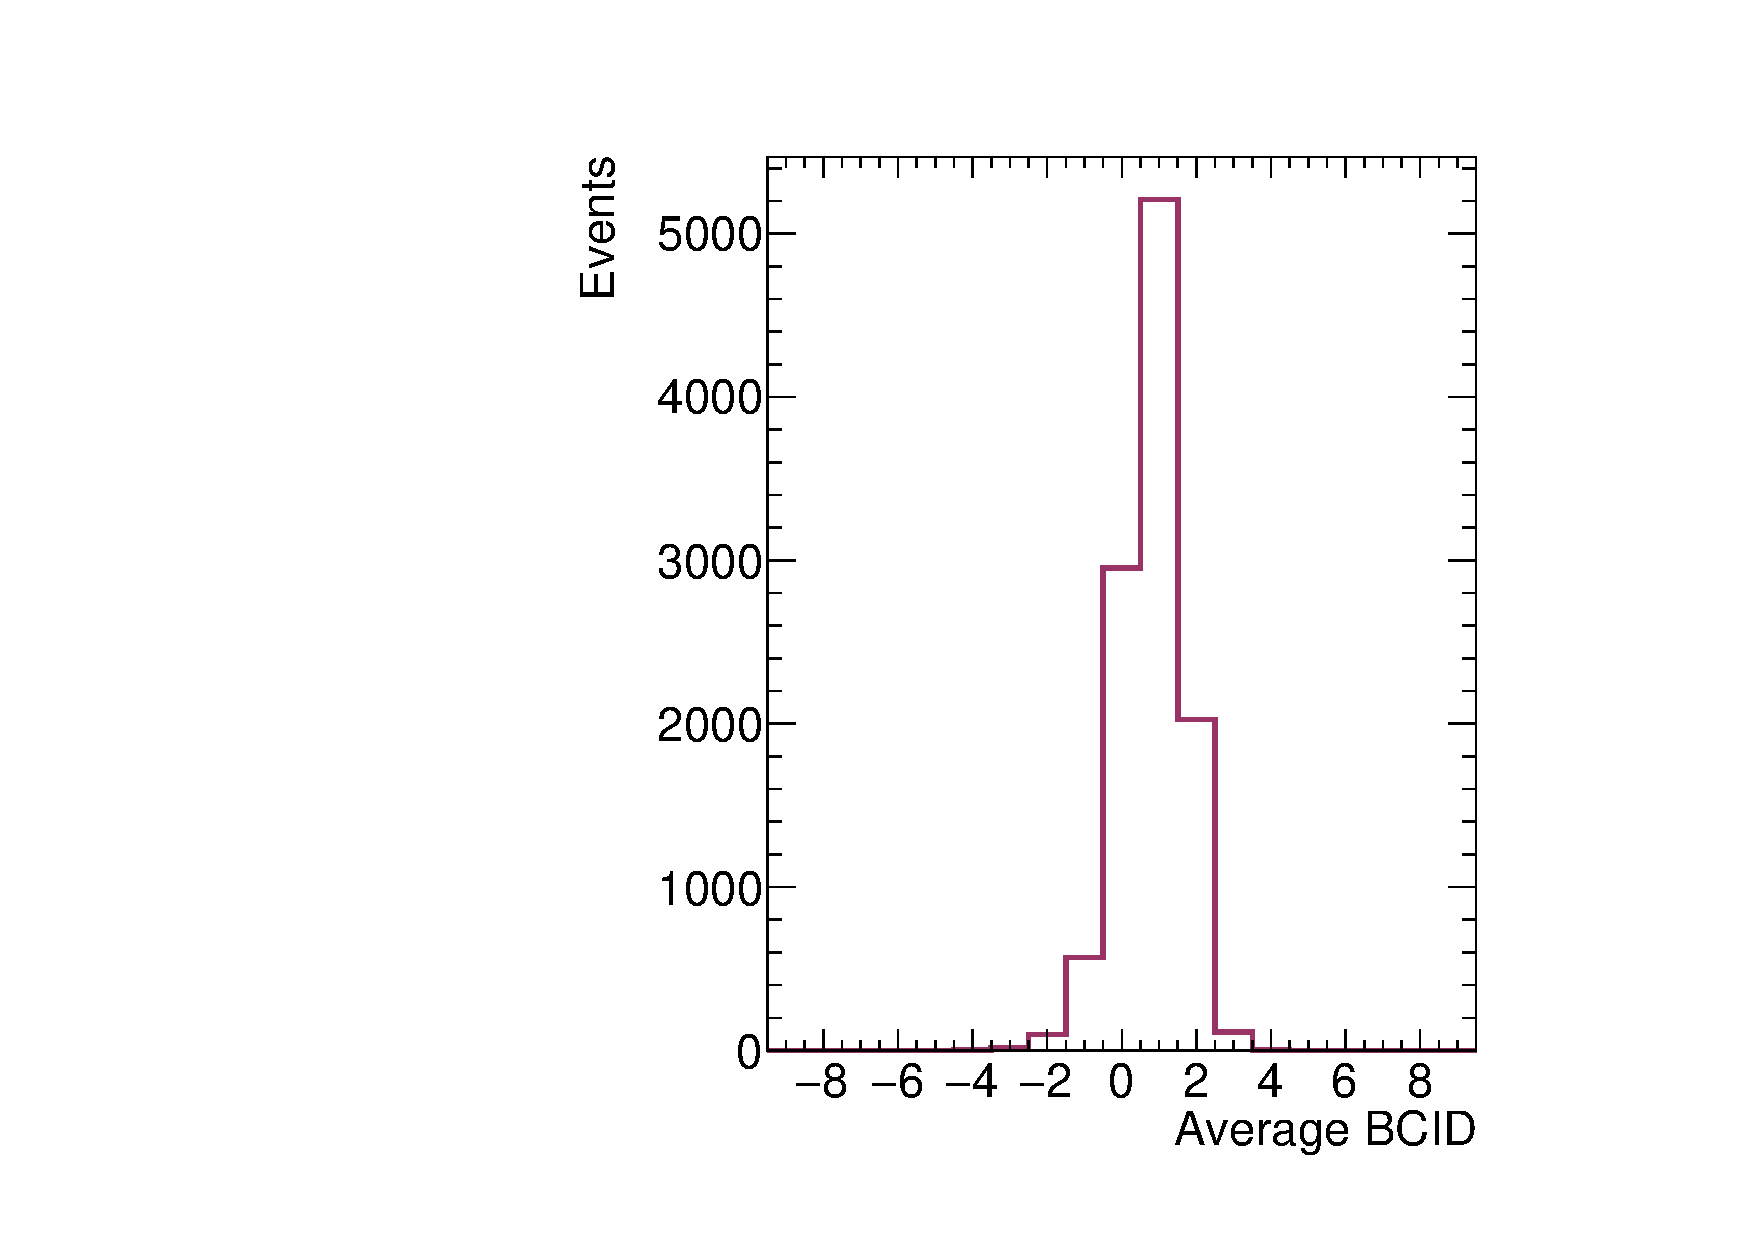
\includegraphics[width=0.3\textwidth]{figures/gbtanalysis3530/avg_BCID.pdf}
    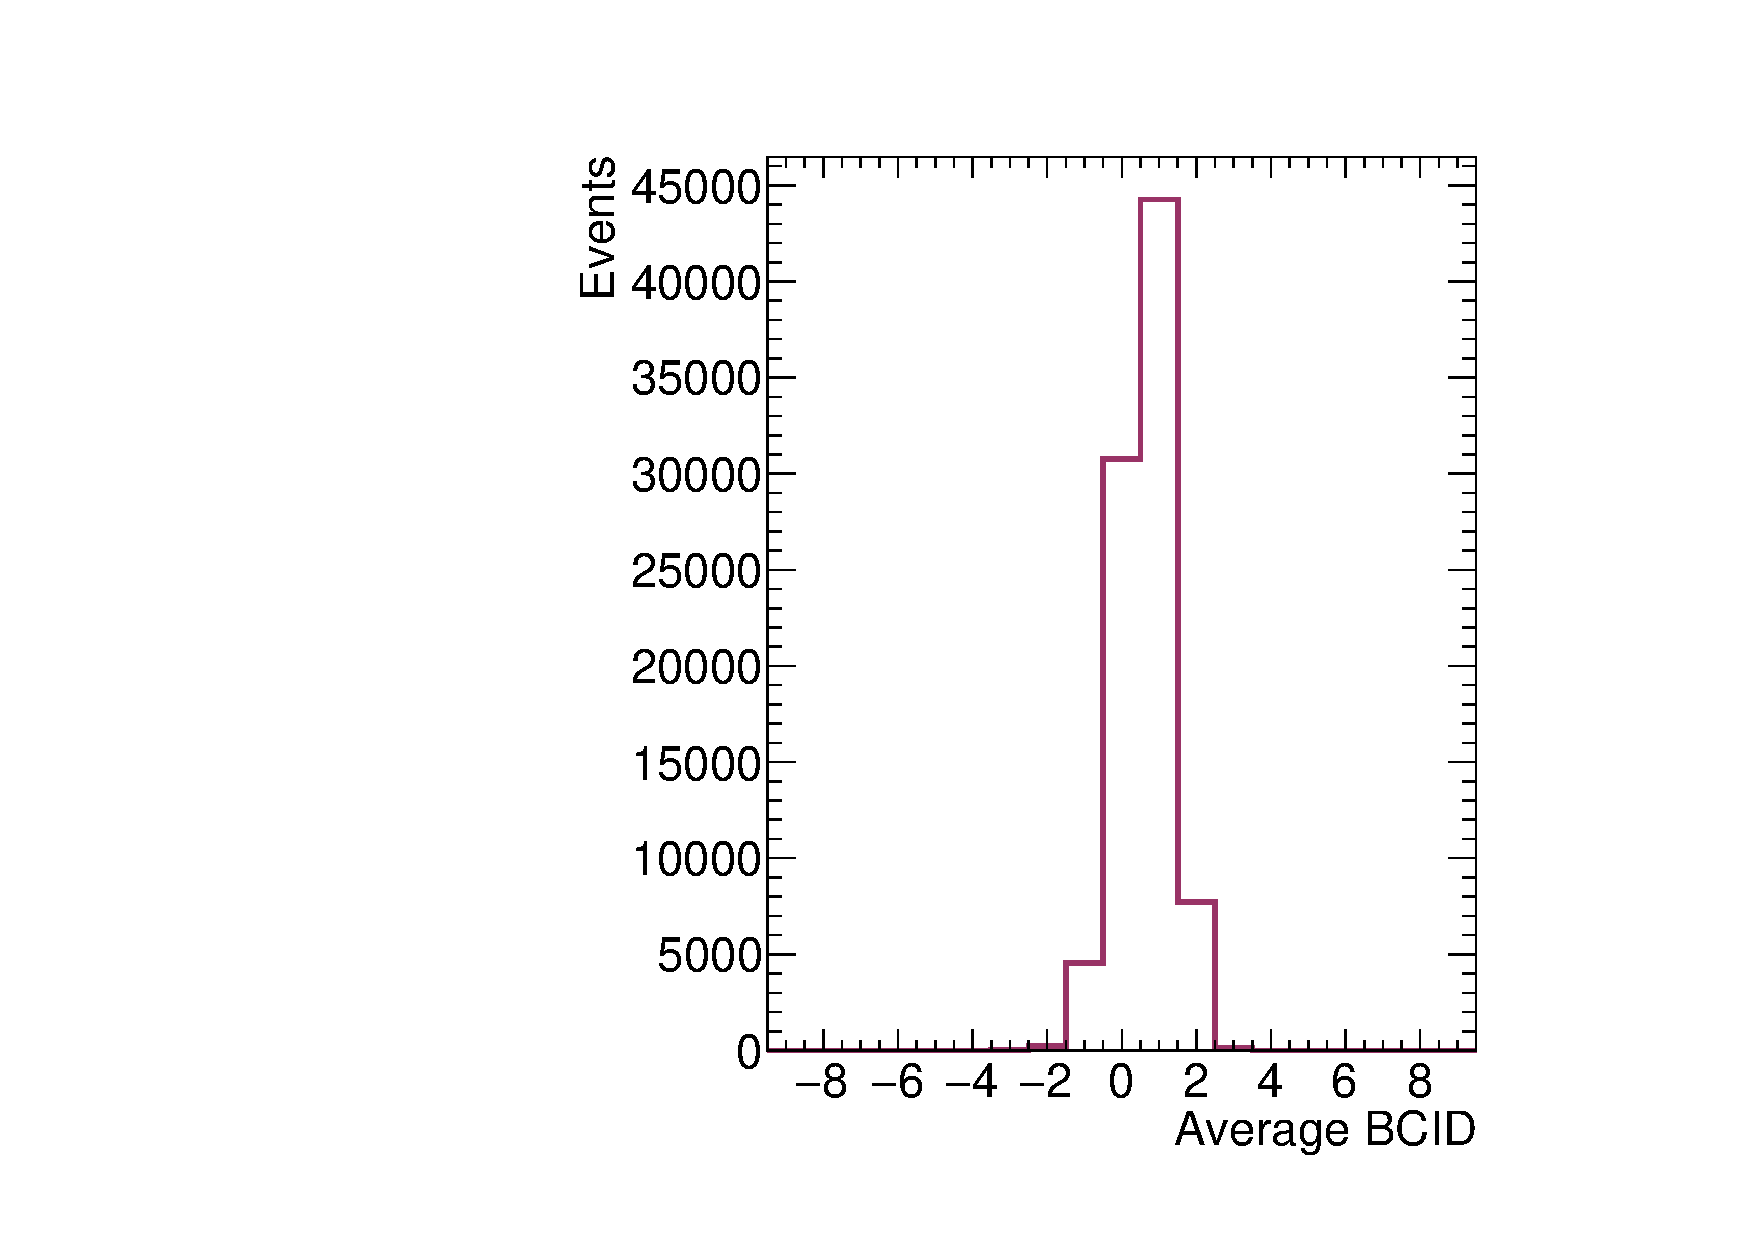
\includegraphics[width=0.3\textwidth]{figures/gbtanalysis3527/avg_BCID.pdf}
    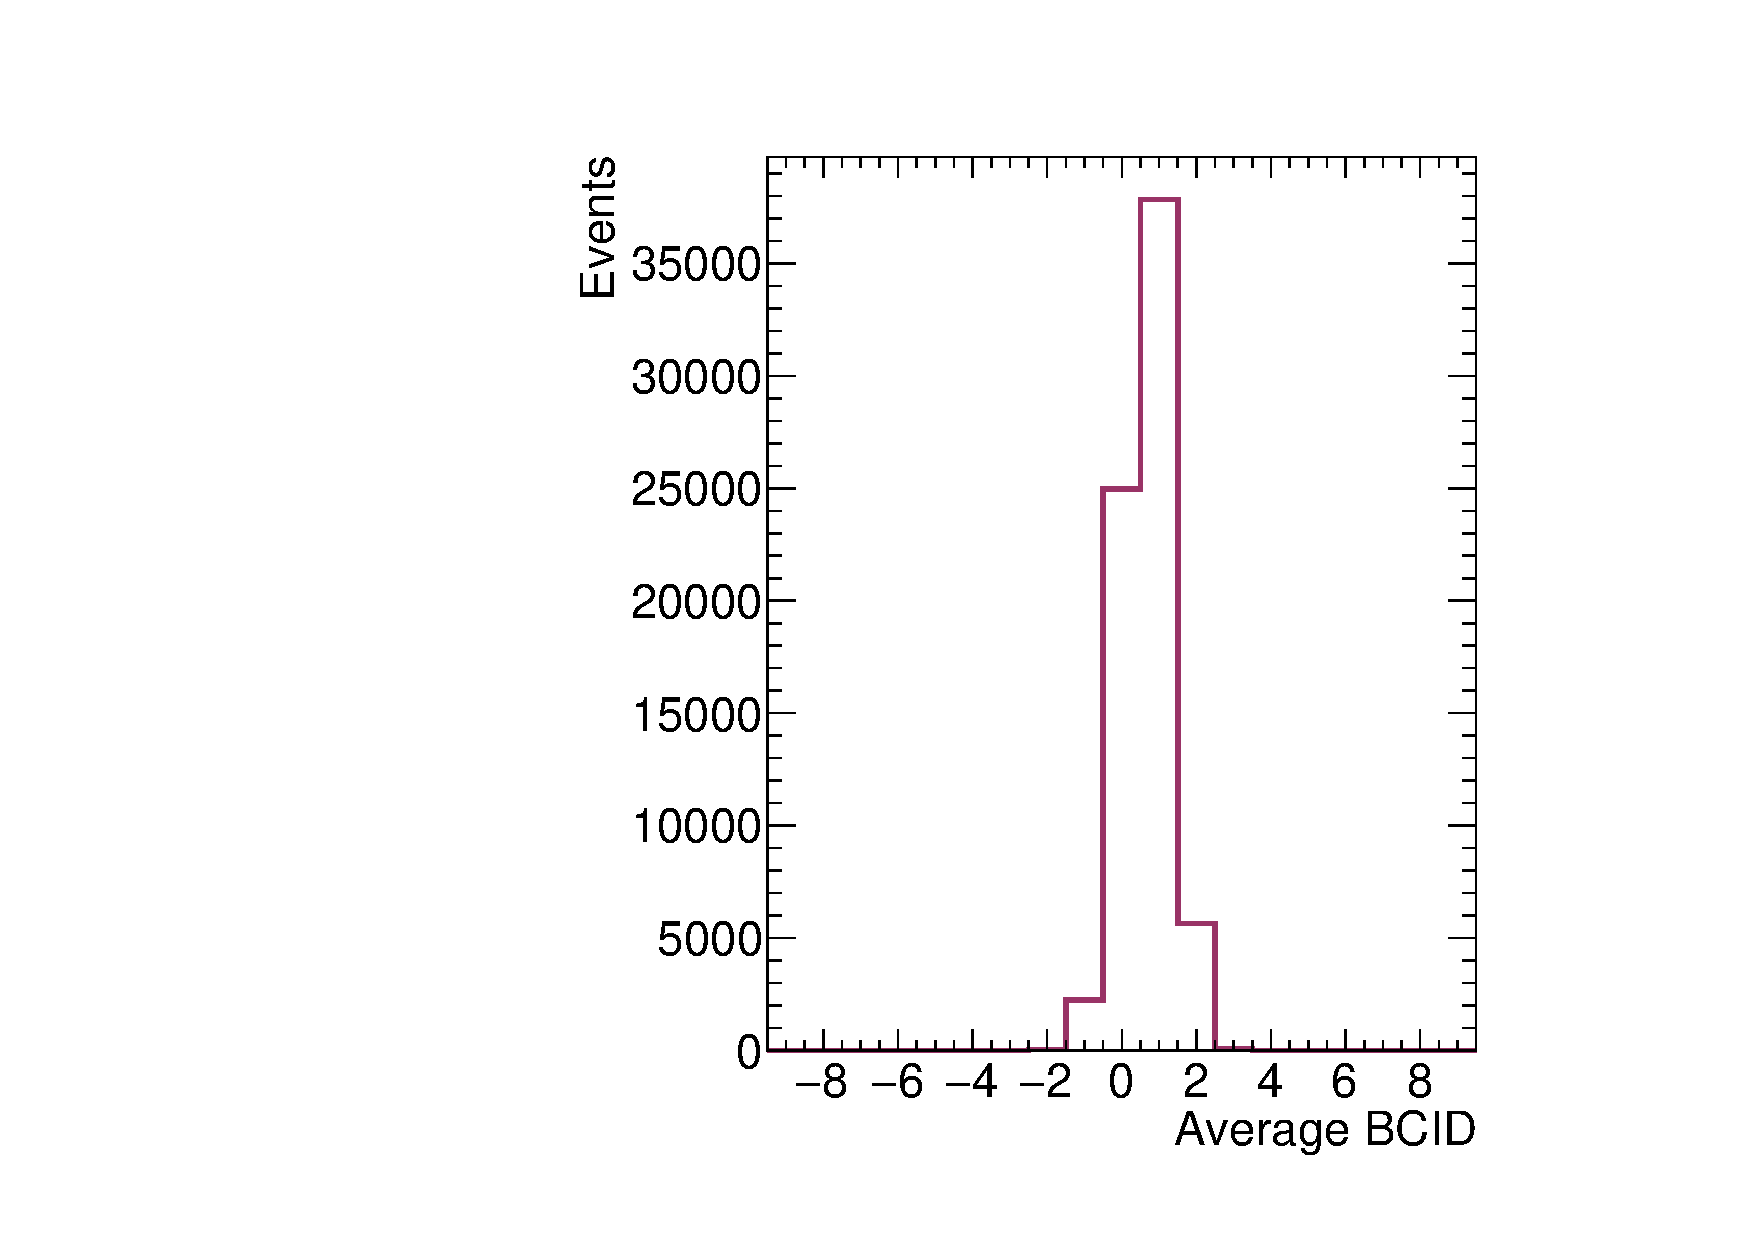
\includegraphics[width=0.3\textwidth]{figures/gbtanalysis3528/avg_BCID.pdf}
  \end{center}
  \vspace{-10pt}
  \caption{The time resolution of the MM TP relative to the scintillator, where the BC of the trigger is defined as the average BCID of the ART hits, for data collected with 200 ns (left), 100 ns (middle), and 50 ns (right) integration time in the VMM.}
  \label{fig:integ_avg_bc}
\end{figure}

\begin{figure}[!htpb]
  \begin{center}
    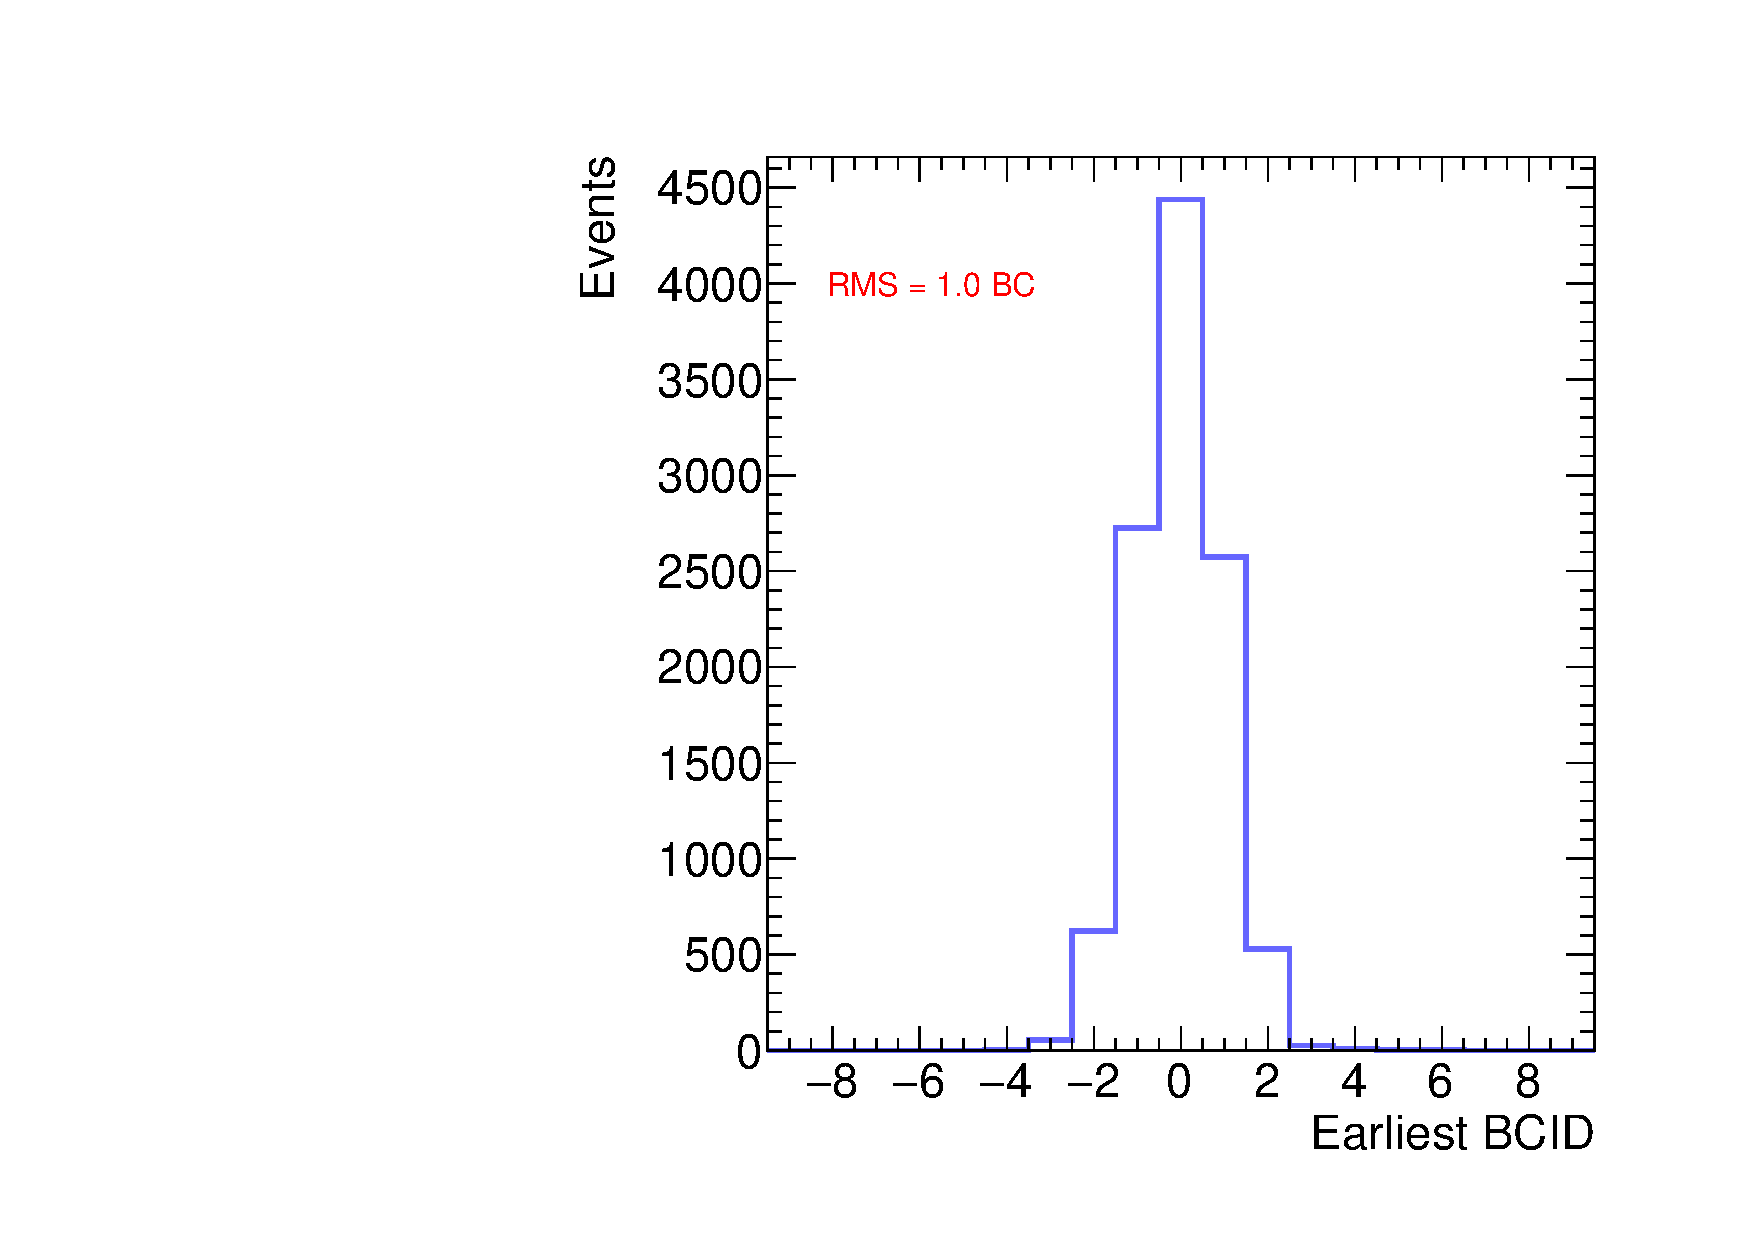
\includegraphics[width=0.3\textwidth]{figures/gbtanalysis3530/earliest_BCID.pdf}
    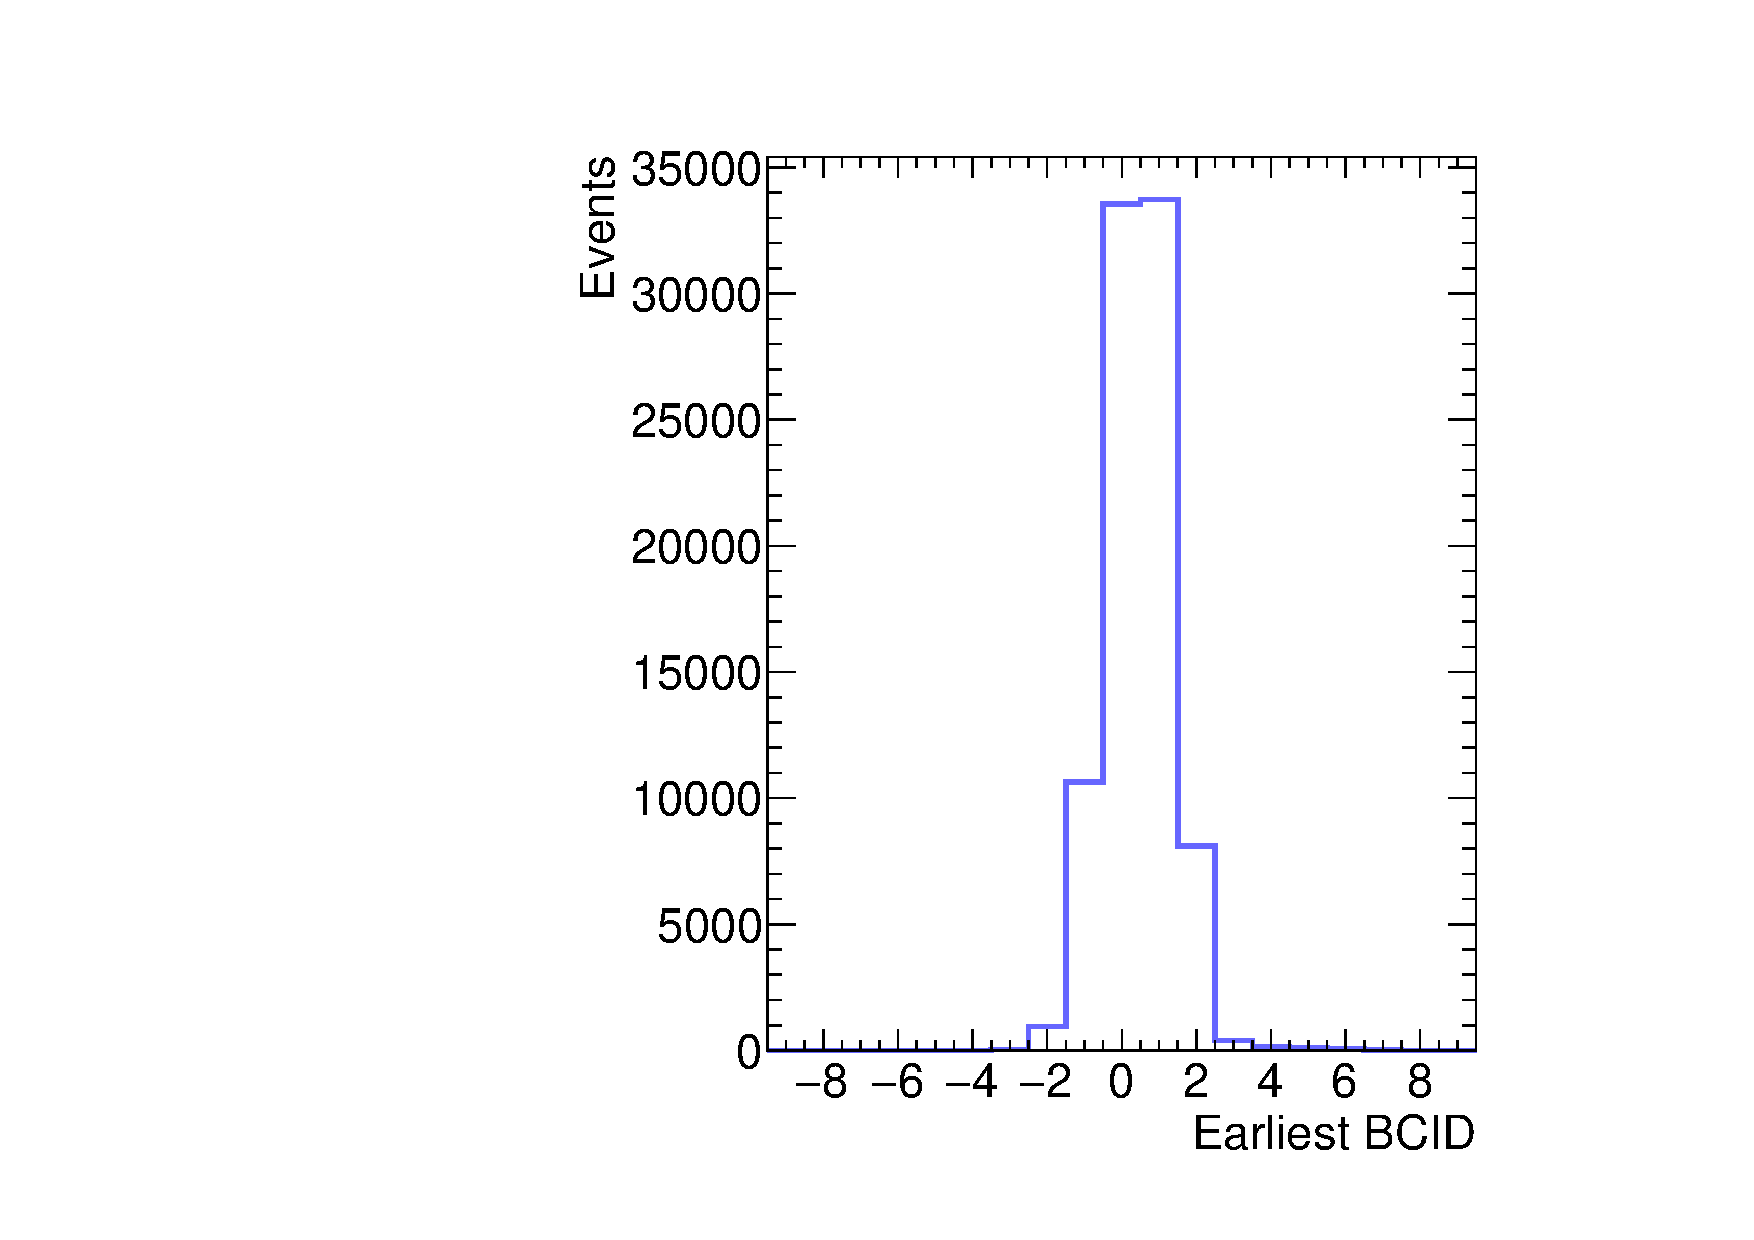
\includegraphics[width=0.3\textwidth]{figures/gbtanalysis3527/earliest_BCID.pdf}
    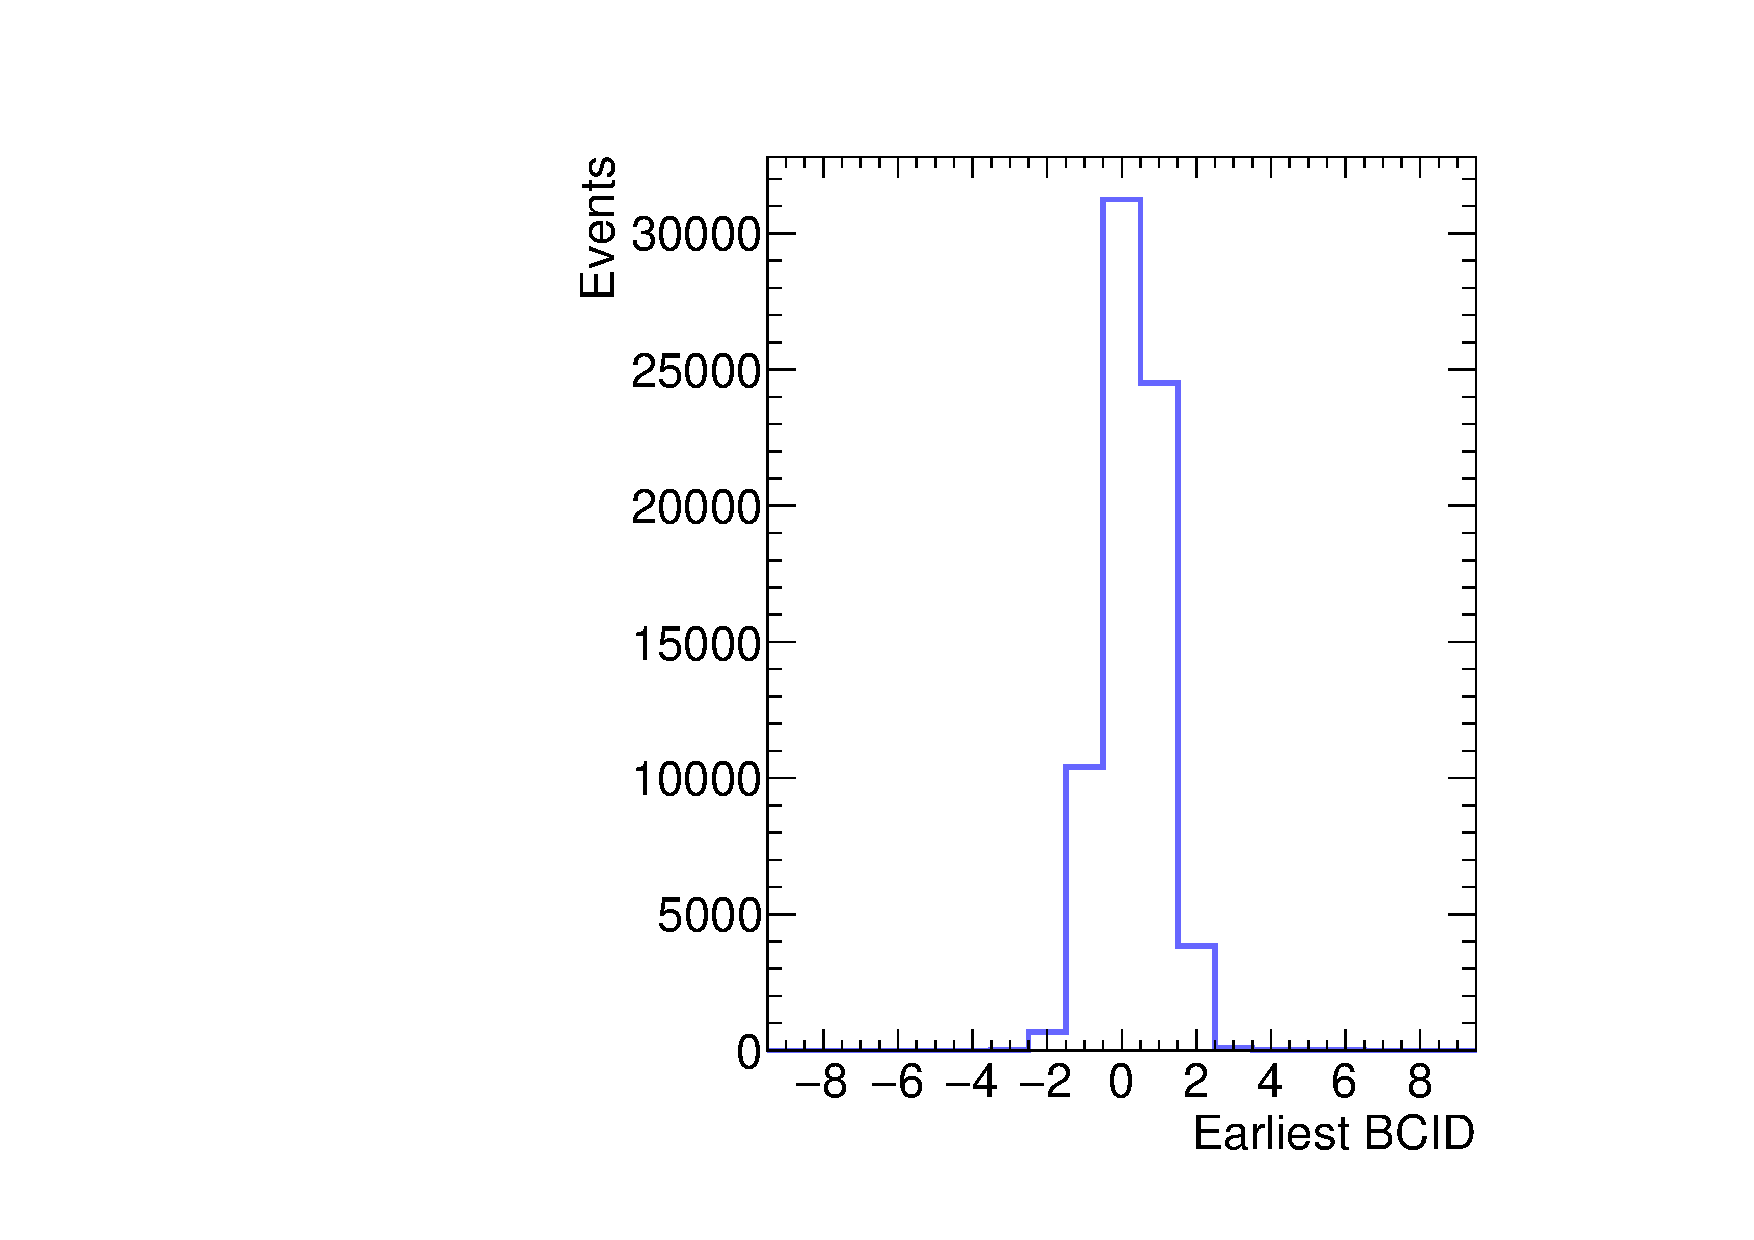
\includegraphics[width=0.3\textwidth]{figures/gbtanalysis3528/earliest_BCID.pdf}
  \end{center}
  \vspace{-10pt}
  \caption{The time resolution of the MM TP relative to the scintillator, where the BC of the trigger is defined as the earliest BCID of the ART hits, for data collected with 200 ns (left), 100 ns (middle), and 50 ns (right) integration time in the VMM.}
  \label{fig:integ_avg_earliest}
\end{figure}


